\chapter{李群、李代数与标准模型}
\label{chap:lie-standard-model}

\chapref{chap:lorentz-poincare} 证明了质量与自旋（或螺旋度）是时空对称性给出的仅有的内禀量子数。但粒子物理中还有电荷、同位旋、色、超荷等大量量子数，它们都来自\textbf{内部对称群}——与时空无关、只在"味空间"或"色空间"里作用的连续群 $SU(2)$、$SU(3)$ 等。把这些连续群、它们的李代数与表示弄明白，才能写出现代粒子物理标准模型的完整群论结构。

这一章有两条任务。第一，把前面特例化的 $SU(2)$ 表示论提升为一套\textbf{适用于任意紧李群}的一般方法：Cartan 子代数、根、权、最高权、Dynkin 图，并用这套方法重新看懂 $SU(2)$ 再推广到 $SU(3)$。第二，把这套方法用于标准模型，写清 $SU(3)_c\times SU(2)_L\times U(1)_Y$ 的规范结构、费米子表示与电荷量子化。

逻辑链是
\[
\text{李代数一般框架}
\longrightarrow \text{根与权}
\longrightarrow SU(2)\text{ 重看}
\longrightarrow SU(3)\text{ 与夸克}
\longrightarrow \text{标准模型}.
\]

\section{李代数的一般框架}


连续对称群的 infinitesimal 结构由 Lie 代数刻画。我们从 Lie 群到 Lie 代数的一般框架开始。

\chapref{chap:rotation-group} 已给出 Lie 群与 Lie 代数的直觉：Lie 群是能以连续参数光滑刻画的群，Lie 代数保留单位元附近的一阶变化，由生成元的交换子刻画局部乘法。这里把要点重述成可用的一般框架。

\begin{definition}[Lie 代数]
实数域（或复数域）上的向量空间 $\mathfrak g$ 配上一个双线性、反对称、满足 Jacobi 恒等式的括积 $[\cdot,\cdot]$，称为\textbf{Lie 代数}：
\[
[X,Y]=-[Y,X],\qquad
[X,[Y,Z]]+[Y,[Z,X]]+[Z,[X,Y]]=0.
\]
Lie 群 $G$ 的李代数 $\mathfrak g=T_eG$ 是单位元处的切空间，括积由群乘法的二阶项给出：把群元写成 $\ee^{X}$，则 $\ee^{X}\ee^{Y}\ee^{-X}\ee^{-Y}=\ee^{[X,Y]+\cdots}$。
\end{definition}

紧 Lie 群的不可约表示具有与有限群完全平行的良好性质：完全可约（Maschke 定理的推广），特征标可由 Weyl 公式计算，维数有 Weyl 维数公式。前几章建立的"不可约表示 → 特征标 → 张量积分解"链条，在紧 Lie 群上逐字成立，只是求和从有限群元的离散和换成群流形上的积分（Haar 测度积分）。


有了 Lie 代数的一般定义，下一步是引入 Cartan 子代数、根与权——这是分类任意紧半单 Lie 群不可约表示的标准工具。

分类紧 Lie 群表示的关键，是把问题归结到一组\textbf{可同时对角化}的生成元上。

\begin{definition}[Cartan 子代数与根]
设 $\mathfrak g$ 是紧 Lie 代数。\textbf{Cartan 子代数} $\mathfrak h\subset\mathfrak g$ 是极大可交换子代数，维数 $r=\operatorname{rank}\mathfrak g$ 称为秩。$\mathfrak h$ 的复化的共同本征空间分解
\[
\mathfrak g_{\CC}=\mathfrak h_{\CC}\oplus\bigoplus_{\alpha\in\Phi}\mathfrak g_\alpha
\]
中，非零本征值 $\alpha\in\mathfrak h^*$（$\alpha\ne0$）称为\textbf{根}，集合 $\Phi$ 称为\textbf{根系}，$\mathfrak g_\alpha=\{X\in\mathfrak g_{\CC}\mid[H,X]=\alpha(H)X,\ \forall H\in\mathfrak h\}$。
\end{definition}

\begin{definition}[权与权空间]
设 $\rho:\mathfrak g\to\mathfrak{gl}(V)$ 是表示。$V$ 分解为 $\mathfrak h$ 的共同本征空间
\[
V=\bigoplus_{\lambda}V_\lambda,\qquad
V_\lambda=\{v\in V\mid\rho(H)v=\lambda(H)v,\ \forall H\in\mathfrak h\}.
\]
本征值 $\lambda\in\mathfrak h^*$ 称为\textbf{权}，$V_\lambda$ 称为权空间，$\dim V_\lambda$ 称为权 $\lambda$ 的\textbf{重数}。表示"按权分解"后，每个不可约表示由它的\textbf{最高权}唯一确定。
\end{definition}

关键事实（不在此证明，但后文处处使用）：不可约表示的权格是离散的；存在唯一\textbf{最高权} $\Lambda$，所有其他权都由 $\Lambda$ 减去正根的非负整数组合得到；不可约表示由其最高权 $\Lambda$ 完全确定。

\begin{proposition}[根空间维数为 1]
对紧 Lie 代数的每个根 $\alpha$，根空间 $\mathfrak g_\alpha$ 是一维的，且 $\alpha$ 的负 $-\alpha$ 也是根。
\end{proposition}

根空间的一维性意味着每个根 $\alpha$ 对应一对升降算符 $E_\alpha\in\mathfrak g_\alpha$、$E_{-\alpha}\in\mathfrak g_{-\alpha}$，它们在表示中的作用与 $SU(2)$ 的 $J_\pm$ 完全平行——这是后文最高权分类定理的基石。但要把"根"从 $\mathfrak h^*$ 中的抽象线性泛函提升为可做几何的对象，还需要一个内积。这个内积来自 Lie 代数自身的不变双线性形式。

\begin{definition}[Killing 形式]
Lie 代数 $\mathfrak g$ 上的 \textbf{Killing 形式}（Cartan--Killing 形式）定义为
\begin{equation}
\label{eq:killing-form}
B(X,Y)=\operatorname{tr}(\operatorname{ad}X\circ\operatorname{ad}Y),\qquad X,Y\in\mathfrak g,
\end{equation}
即线性映射 $\operatorname{ad}X\circ\operatorname{ad}Y:\mathfrak g\to\mathfrak g$ 的迹。
\end{definition}

$B$ 是 $\mathfrak g$ 上的对称双线性形式，且在自同构下不变：$B([X,Y],Z)=B(X,[Y,Z])$（不变性，由 $\operatorname{ad}$ 的表示性质直接给出）。不变性使 $B$ 限制到 Cartan 子代数 $\mathfrak h$ 上给出 $\mathfrak h^*\cong\mathfrak h$ 的自然同构（当 $B$ 非退化时），从而把根 $\alpha\in\mathfrak h^*$ 对应到 $H_\alpha\in\mathfrak h$ 满足 $\alpha(H)=B(H_\alpha,H)$。这就在 $\mathfrak h^*$ 上诱导出内积
\begin{equation}
\label{eq:root-inner-product}
(\alpha,\beta)=B(H_\alpha,H_\beta),
\end{equation}
使根系成为 Euclid 空中的几何对象——这是根图可画的数学基础。

\begin{theorem}[Cartan 半单性判据]
Lie 代数 $\mathfrak g$ 是半单的（不含非零可解理想）当且仅当 Killing 形式 $B$ 非退化。紧 Lie 代数的 Killing 形式是负半定的，且紧半单 Lie 代数的 $B$ 是负定的。
\end{theorem}

\begin{derivation}[Cartan 判据、紧性与 Dynkin 分类的完整推导]
\textbf{第一步：Cartan 可解判据的完整证明.}\enspace 设 $\mathfrak g$ 是特征零域上的有限维 Lie 代数。Lie 定理说：若 $\mathfrak g$ 可解，则其在有限维复表示 $\rho$ 下可同时上三角化——即存在基使所有 $\rho(X)$ 为上三角矩阵。对伴随表示 $\rho=\operatorname{ad}$，可解时所有 $\operatorname{ad}X$ 同时上三角化，故 $\operatorname{ad}X\circ\operatorname{ad}Y$ 也是上三角矩阵，其对角元为 $\operatorname{ad}X$ 与 $\operatorname{ad}Y$ 对角元之积。但 $\operatorname{ad}X$ 上三角化的对角元恰是 $X$ 在根空间分解中的根值 $\alpha(X)$，而可解 Lie 代数的根空间分解中所有根为零（幂零根），故 $\operatorname{ad}X\circ\operatorname{ad}Y$ 的对角元全为零，$B(X,Y)=\tr(\operatorname{ad}X\circ\operatorname{ad}Y)=0$。

反之，若 $B\equiv0$，取 Cartan 子代数 $\mathfrak h$，在根空间分解 $\mathfrak g_\CC=\mathfrak h_\CC\oplus\bigoplus_\alpha\mathfrak g_\alpha$ 下计算 $B$ 。对 $H\in\mathfrak h_\CC$，$\operatorname{ad}H$ 在 $\mathfrak g_\alpha$ 上本征值为 $\alpha(H)$，故
\begin{equation*}
B(H,H')=\sum_{\alpha\in\Phi}\alpha(H)\alpha(H')\,\dim\mathfrak g_\alpha.
\end{equation*}
$B\equiv0$ 迫使所有 $\alpha(H)\alpha(H')=0$，即所有根为零。根全为零意味着 $\mathfrak g_\CC=\mathfrak h_\CC$，即 $\mathfrak g$ 幂零（Cartan 子代数等于全代数），故可解。Killing 形式定义为 $B(X,Y)=\tr(\operatorname{ad}X\circ\operatorname{ad}Y)$，它是对称双线性型且在自同构下不变：$B([Z,X],Y)+B(X,[Z,Y])=0$（由 $\operatorname{ad}([Z,X])=[\operatorname{ad}Z,\operatorname{ad}X]$ 和迹的交换性质直接给出）。

\textbf{第二步：半单等价于 $B$ 非退化——两个方向的完整论证.}\enspace \emph{正向}：若 $\mathfrak g$ 有非零可解理想 $\mathfrak r$（根基），则对 $X\in\mathfrak r$、$Y\in\mathfrak g$，$\operatorname{ad}Y$ 把 $\mathfrak r$ 映入 $\mathfrak r$（$\mathfrak r$ 是理想），$\operatorname{ad}X$ 把 $\mathfrak g$ 映入 $\mathfrak r$（$\mathfrak r$ 是理想），故 $\operatorname{ad}X\circ\operatorname{ad}Y$ 把 $\mathfrak g\to\mathfrak r\to[\mathfrak r,\mathfrak r]\subsetneq\mathfrak r$。迭代导列 $\mathfrak r^{(0)}=\mathfrak r$、$\mathfrak r^{(k+1)}=[\mathfrak r^{(k)},\mathfrak r^{(k)}]$，可解性保证 $\mathfrak r^{(N)}=0$。$\operatorname{ad}X\circ\operatorname{ad}Y$ 把 $\mathfrak g$ 映入 $\mathfrak r^{(1)}$，再复合映入 $\mathfrak r^{(2)}$，\dots，最终映入 $\mathfrak r^{(N)}=0$，故 $\operatorname{ad}X\circ\operatorname{ad}Y$ 幂零，迹为零，$B|_{\mathfrak r\times\mathfrak g}=0$，$B$ 退化。

\emph{反向}：若 $B$ 退化，退化子空间 $\mathfrak r=\{X\mid B(X,Y)=0,\,\forall Y\in\mathfrak g\}$。由不变性 $B([Z,X],Y)=B(X,[Y,Z])=0$（$X\in\mathfrak r$ 时 $[Y,Z]\in\mathfrak g$），故 $[Z,X]\in\mathfrak r$，$\mathfrak r$ 是理想。$B|_{\mathfrak r}=0$，由 Cartan 可解判据 $\mathfrak r$ 可解。$\mathfrak r\ne0$ 意味着 $\mathfrak g$ 有非零可解理想，非半单。这给出半单性的纯代数判据：
\begin{equation*}
\mathfrak g\text{ 半单}\iff\det B\ne0\iff\mathfrak g\cong\bigoplus_i\mathfrak g_i\text{（单理想直和）}.
\end{equation*}
直和分解由 $B$ 非退化给出正交分解 $\mathfrak g=\mathfrak g_1\oplus^\perp\dots\oplus^\perp\mathfrak g_k$，每个 $\mathfrak g_i$ 的 $B|_{\mathfrak g_i}$ 非退化（否则 $\mathfrak g_i$ 有可解理想），故 $\mathfrak g_i$ 单。

\textbf{第三步：紧性给出负定性——从群到代数的正定性传递.}\enspace 紧 Lie 群 $G$ 上取双不变 Riemann 度规（紧群上平均任意度规得到双不变度规）。$\operatorname{Ad}(g)$ 是度规的正交变换：$\langle\operatorname{Ad}(g)X,\operatorname{Ad}(g)Y\rangle=\langle X,Y\rangle$。对 $g=\ee^{tX}$ 求导，得 $\langle\operatorname{ad}X\cdot Y,Z\rangle+\langle Y,\operatorname{ad}X\cdot Z\rangle=0$，即 $\operatorname{ad}X$ 关于正定度规反称。反称矩阵的特征值为纯虚数 $i\lambda_k$（$\lambda_k\in\RR$），$\operatorname{ad}X\circ\operatorname{ad}X$ 的特征值为 $-\lambda_k^2\le0$，故
\begin{equation*}
B(X,X)=\tr(\operatorname{ad}X)^2=\sum_k(-\lambda_k^2)\le0.
\end{equation*}
若 $\mathfrak g$ 半单则 $B$ 非退化，负半定且非退化升级为负定：$B(X,X)<0$（$X\ne0$）。由此，$-B$ 是紧半单 Lie 代数上的正定内积，给出 $\mathfrak h^*$ 上的内积
\begin{equation*}
(\alpha,\beta):=-B(H_\alpha,H_\beta),\qquad H_\alpha\in\mathfrak h\text{ 满足 }\alpha(H)=(H_\alpha,H)\ \forall H\in\mathfrak h.
\end{equation*}
这个内积使根系成为 Euclid 空间中的有限点集，满足严格的几何公理——这是 Dynkin 分类的出发点。

\textbf{第四步：典型 Lie 代数 Killing 形式的显式矩阵计算.}\enspace 对 $\mathfrak{su}(2)$，生成元 $J_i=\sigma_i/2$（$i=1,2,3$），伴随表示 $\operatorname{ad}J_i$ 在基 $\{J_1,J_2,J_3\}$ 下的矩阵为 $(\epsilon_{ijk})_{jk}$（$3\times3$ 反称矩阵）。显式地：
\begin{equation*}
\operatorname{ad}J_1=\begin{pmatrix}0&0&0\\0&0&-1\\0&1&0\end{pmatrix},\quad \operatorname{ad}J_1\circ\operatorname{ad}J_1=\begin{pmatrix}0&0&0\\0&-1&0\\0&0&-1\end{pmatrix},\quad B(J_1,J_1)=\tr=-2.
\end{equation*}
同理 $B(J_i,J_j)=-2\delta_{ij}$，$B=-2\,\tr_{\text{fund}}$，负定非退化，确认 $\mathfrak{su}(2)$ 紧半单。

对 $\mathfrak{su}(3)$，八维生成元 $T_a=\lambda_a/2$（$a=1,\dots,8$），结构常数 $f^{abc}$ 由 $[T_a,T_b]=if^{abc}T_c$ 给出。$\operatorname{ad}T_a$ 在八维伴随表示下的矩阵元 $(\operatorname{ad}T_a)_{bc}=if^{abc}$，$B(T_a,T_b)=\tr(\operatorname{ad}T_a\circ\operatorname{ad}T_b)=-\sum_c f^{abc}f^{abc'}$。利用 $SU(3)$ 的 $f$ 张量恒等式 $\sum_c f^{abc}f^{abc'}=3\delta^{ab}$，得 $B(T_a,T_b)=-3\delta_{ab}$。

一般地，$\mathfrak{su}(N)$ 的 Killing 形式为 $B(X,Y)=-2N\,\tr(XY)$（$\tr$ 为基本表示的迹），负定且非退化。对比：$\mathfrak{u}(1)$ 的 $B\equiv0$（Abelian，$\operatorname{ad}=0$，可解但非半单），$\mathfrak{gl}(N)$ 的 $B$ 退化（有 $\mathfrak{u}(1)$ 中心，$B|_{\text{center}}=0$），均不满足半单条件。$\mathfrak{so}(N)$ 的 $B(X,Y)=-(N-2)\tr(XY)$（$N\ge3$ 时非退化），$\mathfrak{sp}(N)$ 的 $B(X,Y)=-2(N+1)\tr(XY)$——四大经典族的 Killing 形式均为负定，确认它们紧半单。

\textbf{第五步：Weyl 幂幺技巧——复半单与紧实形式的对应.}\enspace Cartan 判据是纯代数的，但物理中需要紧群（表示酉化）。Weyl 幂幺技巧建立复半单 Lie 代数 $\mathfrak g_\CC$ 与其紧实形式 $\mathfrak g_{\text{compact}}$ 的对应：复半单 $\mathfrak g_\CC$ 有 Cartan 分解 $\mathfrak g_\CC=\mathfrak h_\CC\oplus\bigoplus_\alpha\mathfrak g_\alpha$，定义对合 $\omega(E_\alpha)=-E_{-\alpha}$、$\omega(H)=-H$（$H\in\mathfrak h$），则 $\mathfrak g_{\text{compact}}=\{X\in\mathfrak g_\CC\mid\omega(X)=-\bar X\}$ 是紧实形式。例如 $\mathfrak{sl}(N,\CC)$ 的紧实形式是 $\mathfrak{su}(N)$，非紧实形式是 $\mathfrak{sl}(N,\RR)$。复半单 Lie 代数的表示在紧实形式上酉化，故物理中只需研究紧群——这是标准模型规范群取 $SU(N)$ 而非 $SL(N,\CC)$ 的深层原因。

\textbf{第六步：Killing 形式的几何意义与根的长度.}\enspace $-B$ 在 Cartan 子代数 $\mathfrak h$ 上的限制给出 $\mathfrak h^*$ 的内积后，根 $\alpha$ 的长度平方 $|\alpha|^2=-B(H_\alpha,H_\alpha)=\alpha(H_\alpha)$。对 $\mathfrak{su}(2)$，单根 $\alpha$ 满足 $|\alpha|^2=2$（归一化约定），对应 $SU(2)$ 的 $J_\pm$ 升降。对 $\mathfrak{su}(3)$，两个单根 $|\alpha_1|^2=|\alpha_2|^2=2$、$(\alpha_1,\alpha_2)=-1$，夹角 $120^\circ$——正六边形根图的几何完全由 Killing 内积决定。一般地，Cartan 整数 $\langle\alpha,\beta\rangle=2(\alpha,\beta)/(\beta,\beta)\in\ZZ$ 把连续的 Euclid 几何离散化，使根的长度比只能取 $\sqrt{1},\sqrt{2},\sqrt{3}$——这是 Dynkin 分类只有四族加五种例外的根本原因。

Killing 形式非退化时，它在 $\mathfrak h^*$ 上诱导的内积 \eqnrefs{eq:root-inner-product} 使根系满足一组严格的几何公理——这些公理完全决定了 Lie 代数的结构。

\par\smallskip\noindent\textbf{定义（根系公理）.}\enspace Euclid 空间 $E$ 中的有限子集 $\Phi\subset E$ 称为\textbf{根系}（root system），若满足：
\begin{enumerate}[label=(\roman*),leftmargin=3em]
\item $\Phi$ 有限，$0\notin\Phi$，$\Phi$ 张成 $E$；
\item 对每个 $\alpha\in\Phi$，反射 $s_\alpha(\lambda)=\lambda-\frac{2(\lambda,\alpha)}{(\alpha,\alpha)}\alpha$ 保持 $\Phi$ 不变：$s_\alpha(\Phi)=\Phi$；
\item 对所有 $\alpha,\beta\in\Phi$，\textbf{Cartan 整数} $\langle\beta,\alpha\rangle:=\frac{2(\beta,\alpha)}{(\alpha,\alpha)}\in\ZZ$（晶格公理）；
\item 若 $\alpha,c\,\alpha\in\Phi$ 则 $c=\pm1$（既约公理）。
\end{enumerate}
秩 $r=\dim E$。$\Phi$ 的 Weyl 群 $W=\langle s_\alpha:\alpha\in\Phi\rangle$ 是 $O(E)$ 的有限子群。


公理 (ii) 使根系在反射下对称，公理 (iii) 把根的长度比和夹角限制为离散值：由 $\langle\alpha,\beta\rangle\langle\beta,\alpha\rangle=4\cos^2\theta\in\{0,1,2,3\}$，两根的夹角只能是 $0^\circ,30^\circ,45^\circ,60^\circ,90^\circ,120^\circ,135^\circ,150^\circ,180^\circ$，且长度比 $\frac{(\beta,\beta)}{(\alpha,\alpha)}=\frac{\langle\alpha,\beta\rangle}{\langle\beta,\alpha\rangle}\in\{1,2,3,\frac12,\frac13\}$。这些离散约束使根图的几何高度受限——这是 Dynkin 分类可行的根本原因。

根系公理中，"晶格公理"(iii) 是最深刻的：它把连续的 Euclid 几何与离散的整数结构联系起来，使根的长度比只能取 $\sqrt{1},\sqrt{2},\sqrt{3}$ 三种。要利用这一约束进行分类，需要从全根系中提取一组"基"——单根。

\par\smallskip\noindent\textbf{定义（单根与 Cartan 矩阵）.}\enspace 取 $E$ 中一个不与任何根正交的超平面，把 $\Phi$ 分为\textbf{正根} $\Phi^+$ 和\textbf{负根} $\Phi^-=-\Phi^+$。\textbf{单根}（simple roots）$\Delta=\{\alpha_1,\dots,\alpha_r\}$ 是不能写为两个正根之和的正根。单根构成 $\Phi$ 的 $\ZZ$-基：每个正根是单根的非负整系数组合，每个负根是非正整系数组合。\textbf{Cartan 矩阵}定义为
\begin{equation}
\label{eq:cartan-matrix}
A_{ij}=\langle\alpha_j,\alpha_i\rangle=\frac{2(\alpha_j,\alpha_i)}{(\alpha_i,\alpha_i)},\qquad i,j=1,\dots,r.
\end{equation}


Cartan 矩阵满足：$A_{ii}=2$；$A_{ij}\le0$（$i\ne j$）；$A_{ij}=0\Leftrightarrow A_{ji}=0$；且 $A$ 非退化。由 $A_{ij}A_{ji}\in\{0,1,2,3\}$，非对角元编码两单根的夹角与长度比。这一信息可用图形完全编码。

\par\smallskip\noindent\textbf{定义（Dynkin 图）.}\enspace \textbf{Dynkin 图}是编码 Cartan 矩阵的图：每个单根 $\alpha_i$ 对应一个节点；节点 $i,j$（$i\ne j$）之间连 $n_{ij}=A_{ij}A_{ji}\in\{0,1,2,3\}$ 条边。若 $n_{ij}=2$ 或 $3$（两根长度不等），在较长根的节点上画箭头指向较短根。$n_{ij}=0$（正交）不连线，$n_{ij}=1$（等长、$120^\circ$）连单线，$n_{ij}=2$（$\sqrt2$ 长度比、$135^\circ$）连双线，$n_{ij}=3$（$\sqrt3$ 长度比、$150^\circ$）连三线。


\par\smallskip\noindent\textbf{定理（Dynkin 分类定理）.}\enspace 既约根系（不可分解为两个正交子根系之并）的 Dynkin 图恰为以下类型之一：
\begin{center}
\begin{tabular}{lll}
\toprule
类型 & Dynkin 图 & 对应紧单 Lie 群 \\
\midrule
$A_r$（$r\ge1$） & 单链 $r$ 节点 & $SU(r+1)$ \\
$B_r$（$r\ge2$） & 单链 $r$ 节点，末端双线 & $SO(2r+1)$ \\
$C_r$（$r\ge3$） & 单链 $r$ 节点，末端双线（箭头反向） & $Sp(r)$ \\
$D_r$（$r\ge4$） & 单链 $r-2$ 节点，末端分叉 & $SO(2r)$ \\
$E_6,E_7,E_8$ & 例外图 & 例外群 \\
$F_4$ & $3$ 节点单链 $+$ 双线 & 例外群 \\
$G_2$ & $2$ 节点三线 & 例外群 \\
\bottomrule
\end{tabular}
\end{center}
每个紧半单 Lie 代数唯一分解为单理想的直和，对应 Dynkin 图的连通分量之并。


\textbf{第一步：单根的约束——无环引理.}\enspace 单根集 $\Delta$ 满足：(a) $(\alpha_i,\alpha_j)\le0$（$i\ne j$）——否则 $\alpha_i-\alpha_j$ 是根，与单根定义矛盾；(b) $\Delta$ 中不含三个两两非正交的根——否则它们张成 $2$ 维子空间，与秩 $r=\dim E$ 矛盾。由此，Dynkin 图中无环（回路）：若有环 $\alpha_1-\alpha_2-\dots-\alpha_k-\alpha_1$，则环上每个节点至少两条边，环内区域的 Cartan 矩阵子块行列式 $\le0$，与正定性矛盾。具体地，环上 $k$ 个根的 Gram 矩阵
\begin{equation*}
G_{ij}=(\alpha_i,\alpha_j)
\end{equation*}
是 $k\times k$ 半正定矩阵，但环约束使 $\det G=0$（线性相关），与 $B$ 正定矛盾。

\textbf{第二步：双线/三线的限制——角度与长度比的离散约束.}\enspace 含双线的既约图至多一条双线：两条双线会迫使含环。含三线至多一条三线（$G_2$），且三线图不能同时含双线。角度与长度比的约束来自 Cartan 整数：
\begin{equation*}
\langle\alpha_i,\alpha_j\rangle\langle\alpha_j,\alpha_i\rangle=4\cos^2\theta_{ij}\in\{0,1,2,3\},
\end{equation*}
故 $\theta_{ij}\in\{90^\circ,120^\circ,135^\circ,150^\circ\}$（非正交单根间），对应 $0,1,2,3$ 条边。长度比
\begin{equation*}
\frac{|\alpha_i|}{|\alpha_j|}=\sqrt{\frac{\langle\alpha_j,\alpha_i\rangle}{\langle\alpha_i,\alpha_j\rangle}}\in\{1,\sqrt2,\sqrt3\},
\end{equation*}
由箭头方向编码（箭头指向短根）。$G_2$ 的两根长度比 $\sqrt3$，夹角 $150^\circ$，Cartan 矩阵
\begin{equation*}
A_{G_2}=\begin{pmatrix}2&-1\\-3&2\end{pmatrix},\qquad \det A_{G_2}=1>0.
\end{equation*}

\textbf{第三步：分叉的限制——$D$ 系列与 $E$ 系列.}\enspace 分叉点（一个节点连三条单线）至多一个：两个分叉点会迫使含环。分叉图不能再含双线/三线（否则度数过高）。计算各分叉臂的长度约束：设分叉点连三条臂，各臂长度（节点数）为 $(a,b,c)$，则 Cartan 矩阵的正定性等价于
\begin{equation*}
\frac{1}{a+1}+\frac{1}{b+1}+\frac{1}{c+1}>1.
\end{equation*}
此不等式来自分叉点处 Gram 矩阵的子行列式。整数解只有：
\begin{equation*}
(1,1,1)\to D_4,\quad (2,1,1)\to D_5,\quad (2,2,1)\to E_6,\quad (3,2,1)\to E_7,\quad (3,2,1)\to E_8.
\end{equation*}
$E_8$ 臂长 $(3,2,1)$ 加分叉点共 $8$ 节点，$1/4+1/3+1/2=13/12>1$ 成立，$E_8$ 的 Cartan 矩阵 $\det=1>0$。

\textbf{第四步：穷举与确认——四族经典加五种例外.}\enspace 无分叉、无双三线的连通图只能是：(a) 纯单链 $A_r$（$r$ 节点，$SU(r+1)$）；(b) 单链末端一条双线 $B_r$（$SO(2r+1)$）或 $C_r$（$Sp(r)$）；(c) 单链末端分叉 $D_r$（$SO(2r)$，$r\ge4$）；(d) $E_6,E_7,E_8$；(e) $F_4$；(f) $G_2$。每种图对应唯一既约根系，进而唯一紧单 Lie 代数。完备性来自：任何连通无环图只含上述形式，且每种图的 Cartan 矩阵正定。

\textbf{第五步：典型 Cartan 矩阵的显式验证与物理对应.}\enspace $A_2$（$SU(3)$）：
\begin{equation*}
A=\begin{pmatrix}2&-1\\-1&2\end{pmatrix},\qquad \det A=3>0.
\end{equation*}
$B_2$（$SO(5)$）：
\begin{equation*}
A=\begin{pmatrix}2&-1\\-2&2\end{pmatrix},\qquad \det A=2>0.
\end{equation*}
$A_r$（$SU(r+1)$）：三对角矩阵，$\det A=r+1>0$。$D_r$（$SO(2r)$）：$\det A=4>0$（$r\ge4$）。物理中 $A_r$ 给出 $SU(r+1)$ 规范群（标准模型 $SU(3)\times SU(2)$ 属 $A_2\times A_1$），$D_r$ 给出 $SO(2r)$（大统一 $SO(10)$ 属 $D_5$），$E_6,E_8$ 在弦论紧致化中出现，$G_2$ 在 M 理论中出现。

\textbf{第六步：Dynkin 分类对表示论的意义.}\enspace Dynkin 分类不仅给出 Lie 代数的完整列表，还直接决定了表示论的结构：每个紧单 Lie 群的不可约表示由支配整权 $\Lambda\in P^+$ 参数化，而 $P^+$ 由 Cartan 矩阵（即 Dynkin 图）完全决定。因此，Dynkin 图同时编码了\emph{群的结构}（交换子 $[E_{\alpha_i},E_{-\alpha_j}]=\delta_{ij}H_{\alpha_i}$）和\emph{表示的分类}（最高权 $\langle\Lambda,\alpha_i^\vee\rangle\in\NN$）。对 $SU(3)$（$A_2$），$P^+=\{(p,q):p,q\in\NN\}$ 给出全部不可约表示 $\mathbf{1},\mathbf{3},\bar{\mathbf{3}},\mathbf{6},\mathbf{8},\mathbf{10},\dots$。对 $E_8$（秩 $8$），$P^+$ 是 $8$ 维非负整格，$E_8$ 的最小非平凡表示维数 $248$（伴随表示），$E_8$ 的根格等于权格——这是 $E_8$ 在弦论中特殊的根源。


\textbf{第十二步：例外群的构造与性质.}\enspace 例外群的显式构造：(a) $G_2=\operatorname{Aut}(\mathbb O)$（八元数自同构群，$14$ 维，最小例外单 Lie 代数），根系有 $12$ 个根（长根 $6$ 个、短根 $6$ 个），Cartan 矩阵 $\begin{pmatrix}2&-1\\-3&2\end{pmatrix}$；(b) $F_4$（$52$ 维，含 $G_2$ 子代数），基本表示 $26$ 维（由八元数 Jordan 代数 $J_3(\mathbb O)$ 的自同构给出）；(c) $E_6$（$78$ 维，$27$ 维基本表示，大统一模型候选），$E_7$（$133$ 维，$56$ 维基本表示），$E_8$（$248$ 维，只有伴随表示，根格自对偶 $\det=1$）。$E_8$ 在弦理论中特殊：$E_8\times E_8$ 异化弦规范群，$E_8$ 根格的偶性（even lattice）保证规范反常自动抵消。\end{derivation}

Dynkin 分类是 Lie 理论最深刻的定理之一：它把"所有可能的连续对称群"完全枚举出来。物理中遇到的 $SU(N)$（$A_{N-1}$）、$SO(N)$（$B/D$ 系列）、$Sp(N)$（$C$ 系列）对应四大经典族，而 $E_6,E_7,E_8,F_4,G_2$ 是五种例外群——$E_8$ 在弦理论和 M 理论中扮演核心角色。

分类完成后，回到表示论的核心问题：不可约表示如何标记？答案涉及权格与支配权。

\begin{definition}[权格与支配权]
设 $\Delta=\{\alpha_1,\dots,\alpha_r\}$ 为单根。\textbf{基本权} $\omega_1,\dots,\omega_r\in\mathfrak h^*$ 由 $\langle\omega_i,\alpha_j^\vee\rangle:=\frac{2(\omega_i,\alpha_j)}{(\alpha_j,\alpha_j)}=\delta_{ij}$ 定义（$\alpha_j^\vee=2\alpha_j/(\alpha_j,\alpha_j)$ 为对偶根）。\textbf{权格} $P=\sum_{i=1}^r\ZZ\,\omega_i$ 是所有可能权的集合。\textbf{支配整权}（dominant integral weights）$P^+=\sum_{i=1}^r\NN\,\omega_i$（非负整系数组合）构成最高权的候选集。
\end{definition}

\begin{theorem}[最高权分类定理]
紧半单 Lie 群 $G$ 的不可约复表示与支配整权 $\Lambda\in P^+$ 之间存在自然双射 $\Lambda\mapsto V(\Lambda)$。$\Lambda$ 是 $V(\Lambda)$ 的唯一最高权，$\dim V(\Lambda)$ 由 Weyl 维数公式给出。表示 $V(\Lambda)$ 的所有权由 Weyl 群作用于 $\Lambda$ 生成，形如 $\Lambda-\sum_i n_i\alpha_i$（$n_i\in\NN$）。
\end{theorem}

\begin{derivation}[最高权分类、Freudenthal 公式与 Peter--Weyl 定理]
\textbf{第一步：最高权向量的存在性与定义.}\enspace 在表示 $V$ 中取一个权 $\lambda$ 使 $\lambda+\alpha_i$ 不是权（对所有单根 $\alpha_i$）。对应的权向量 $v_\lambda$ 被 $E_{\alpha_i}$ 湮灭（$E_{\alpha_i}v_\lambda=0$），称为\textbf{最高权向量}。有限维表示的权集有限，故最高权向量总存在。权向量满足
\begin{equation*}
H v_\lambda=\lambda(H)v_\lambda\quad(\forall H\in\mathfrak h),\qquad E_{\alpha_i}v_\lambda=0\quad(\forall i).
\end{equation*}
最高权的存在性也可从 Weyl 群对称性看出：权集在 Weyl 群作用下不变，取 Weyl 室中偏序的极大元即为最高权。

\textbf{第二步：由最高权向量生成的子表示——降权链的构造.}\enspace 令 $V'=\operatorname{span}\{E_{-\alpha_{i_1}}\cdots E_{-\alpha_{i_k}}v_\lambda:k\ge0,\,i_j\in\{1,\dots,r\}\}$。由 $[E_{\alpha_i},E_{-\alpha_j}]\in\mathfrak h$（$i=j$）或 $\mathfrak g_{\alpha_i-\alpha_j}$（$i\ne j$），$E_{\alpha_i}$ 作用在 $V'$ 的生成元上仍给出 $V'$ 中元素，故 $V'$ 在 $\mathfrak g$ 下不变，是不可约子表示。权集为
\begin{equation*}
\mathrm{Wt}(V')=\{\lambda-\textstyle\sum_i n_i\alpha_i:n_i\in\NN\}\cap\mathrm{Wt}(V).
\end{equation*}
每个生成元 $E_{-\alpha_{i_1}}\cdots E_{-\alpha_{i_k}}v_\lambda$ 的权为
\begin{equation*}
\lambda-\alpha_{i_1}-\dots-\alpha_{i_k},
\end{equation*}
即从最高权 $\lambda$ 沿根格向下走。$V'$ 的不可约性来自：$v_\lambda$ 在 $\mathfrak g$ 作用下生成的空间已是最小不变子空间。

\textbf{第三步：支配性条件——$SU(2)$ 子代数的约束.}\enspace 对每个单根 $\alpha_i$，子代数 $\mathfrak g_i=\langle H_{\alpha_i},E_{\pm\alpha_i}\rangle\cong\mathfrak{su}(2)$ 在 $V$ 上的限制给出 $SU(2)$ 表示。最高权向量 $v_\lambda$ 是这个 $SU(2)$ 的最高权向量，权为
\begin{equation*}
\langle\lambda,\alpha_i^\vee\rangle=\frac{2(\lambda,\alpha_i)}{(\alpha_i,\alpha_i)}.
\end{equation*}
$SU(2)$ 表示的最高权必须是非负整数，故
\begin{equation*}
\langle\lambda,\alpha_i^\vee\rangle\in\NN\quad(\forall i),
\end{equation*}
即 $\lambda\in P^+$（支配整权）。物理上，$SU(2)$ 子代数对应每个单根方向的"角动量"，支配性条件要求每个方向的角动量量子数为半整数。

\textbf{第四步：双射——分类定理的完成.}\enspace 两个不同支配整权 $\Lambda\ne\Lambda'$ 给出不同表示，且每个不可约表示有唯一最高权，故 $\Lambda\mapsto V(\Lambda)$ 是 $P^+$ 到不可约表示集的双射。$\dim V(\Lambda)$ 由 Weyl 维数公式计算：
\begin{equation*}
\dim V(\Lambda)=\prod_{\alpha\in\Phi^+}\frac{(\Lambda+\rho,\alpha)}{(\rho,\alpha)},\qquad \rho=\tfrac12\textstyle\sum_{\alpha\in\Phi^+}\alpha.
\end{equation*}
存在性由 Verma 模构造给出：Verma 模 $M(\Lambda)=U(\mathfrak g)\otimes_{U(\mathfrak b)}\CC_\Lambda$ 有唯一极大子模，商模 $V(\Lambda)=M(\Lambda)/N$ 是最高权 $\Lambda$ 的不可约表示。

\textbf{第五步：权集的 Weyl 群对称性与重数公式.}\enspace $V(\Lambda)$ 的权集在 Weyl 群 $W$ 作用下不变：若 $\mu$ 是权则 $w\cdot\mu$ 也是权，且重数 $m(w\cdot\mu)=m(\mu)$。权集的形状由最高权 $\Lambda$ 和 Weyl 群轨道决定：所有权落在凸包
\begin{equation*}
\operatorname{conv}\{w\cdot\Lambda:w\in W\}
\end{equation*}
内（Weyl 凸性定理），且每个 Weyl 轨道中恰有一个支配权。权重数由 Freudenthal 递推公式计算，从 $m(\Lambda)=1$ 出发逐步降权。

\textbf{第六步：物理实例——$SU(2)$ 与 $SU(3)$ 的权图.}\enspace $SU(2)$（秩 $1$）：$P^+=\{0,\frac12,1,\frac32,\dots\}$，Dynkin 记号 $(n)$ 对应 $j=n/2$，$\dim=2j+1=n+1$。权图是一维链 $\{-j,-j+1,\dots,j\}$，Weyl 群 $\ZZ_2$（翻转 $\mu\to-\mu$）。

$SU(3)$（秩 $2$）：$P^+=\{(p,q):p,q\in\NN\}$，
\begin{equation*}
\dim(p,q)=\tfrac12(p+1)(q+1)(p+q+2).
\end{equation*}
$\mathbf{3}=(1,0)$（夸克）、$\bar{\mathbf{3}}=(0,1)$（反夸克）、$\mathbf{8}=(1,1)$（胶子/伴随）、$\mathbf{10}=(3,0)$（重子十重态）、$\mathbf{6}=(2,0)$（对称双夸克）、$\mathbf{27}=(2,2)$（$8\otimes8$ 分解中的最大表示）——标准模型的全部表示内容由 $P^+$ 的支配整权枚举给出。Weyl 群 $S_3$（正六边形对称）作用于权图，给出权集的 $D_3$ 对称性。

最高权分类把"找所有不可约表示"化为"找所有支配整权"——一个纯组合问题。对 $SU(2)$，$P^+=\{0,\frac12\omega,1\cdot\omega,\frac32\omega,\dots\}$ 对应 $j=0,\frac12,1,\frac32,\dots$；对 $SU(3)$，$P^+=\{p\,\omega_1+q\,\omega_2:p,q\in\NN\}$ 对应 Dynkin 记号 $(p,q)$。

不可约表示的权集已知，但每个权的\emph{重数}（multiplicity）——即权空间的维数——如何计算？这是比分类更精细的问题，答案由 Freudenthal 公式给出。

\par\smallskip\noindent\textbf{定理（Freudenthal 权重数公式）.}\enspace 设 $V(\Lambda)$ 是最高权 $\Lambda$ 的不可约表示，$\rho=\frac12\sum_{\alpha\in\Phi^+}\alpha$ 是 Weyl 向量。权 $\mu$ 的重数 $m(\mu)=\dim V_\mu$ 满足递推
\begin{equation}
\label{eq:freudenthal}
\bigl(|\Lambda+\rho|^2-|\mu+\rho|^2\bigr)\,m(\mu)=2\sum_{\alpha\in\Phi^+}\sum_{k\ge1}(\mu+k\alpha,\alpha)\,m(\mu+k\alpha),
\end{equation}
其中 $m(\mu)=0$ 若 $\mu$ 不是权。从 $m(\Lambda)=1$ 出发，逐步降权递推即可算出所有权重数。


\textbf{第一步：Casimir 算符的本征值——二次不变量的作用.}\enspace 二次 Casimir 算符
\begin{equation*}
C=\sum_i H_i^2+\sum_{\alpha\in\Phi^+}(E_\alpha E_{-\alpha}+E_{-\alpha}E_\alpha)
\end{equation*}
（$H_i$ 为 $\mathfrak h$ 的 $-B$-正交基）是与所有 $\mathfrak g$ 元交换的不变量，故在不可约表示 $V(\Lambda)$ 上取常值本征值。在最高权向量 $v_\Lambda$ 上：$E_\alpha v_\Lambda=0$（$\alpha>0$），用 $\rho$ 位移：
\begin{equation*}
C v_\Lambda=(|\Lambda+\rho|^2-|\rho|^2)v_\Lambda,\qquad \rho=\tfrac12\textstyle\sum_{\alpha>0}\alpha.
\end{equation*}
对任意 $v\in V_\mu$，$Cv=(|\Lambda+\rho|^2-|\rho|^2)v$。

\textbf{第二步：在权空间上分解 Casimir——迹的计算.}\enspace 把 $C$ 限制到 $V_\mu$ 上取迹。$\mathfrak h$ 部分贡献 $|\mu|^2\,m(\mu)$（$m(\mu)=\dim V_\mu$）。正根部分用 $E_\alpha E_{-\alpha}+E_{-\alpha}E_\alpha=E_{-\alpha}E_\alpha+H_\alpha$。$E_{-\alpha}E_\alpha$ 把 $V_\mu$ 映到 $V_{\mu-\alpha}\to V_\mu$，其迹为
\begin{equation*}
\sum_{k\ge1}(\mu+k\alpha,\alpha)\,m(\mu+k\alpha),
\end{equation*}
由 $E_\alpha$ 在权链上的 $SU(2)$ 表示矩阵元计算：权链 $\mu,\mu+\alpha,\dots,\mu+k\alpha$ 上 $E_\alpha$ 的作用由 $SU(2)$ 的 $J_+$ 矩阵元给出，
\begin{equation*}
|E_\alpha v_{\mu+k\alpha}|^2=(\mu+k\alpha,\alpha)\,m(\mu+k\alpha).
\end{equation*}
$H_\alpha$ 部分贡献 $(\mu,\alpha)\,m(\mu)$，求和后与 $k=0$ 项合并。

\textbf{第三步：整理递推——Freudenthal 公式的导出.}\enspace 等式 $C$ 的本征值等于 $C$ 在 $V_\mu$ 上的迹：
\begin{equation*}
(|\Lambda+\rho|^2-|\rho|^2)\,m(\mu)=|\mu|^2\,m(\mu)+2\sum_{\alpha\in\Phi^+}\sum_{k\ge1}(\mu+k\alpha,\alpha)\,m(\mu+k\alpha)+\sum_{\alpha>0}(\mu,\alpha)\,m(\mu).
\end{equation*}
利用 $\sum_{\alpha>0}(\mu,\alpha)=(\mu,2\rho)$ 和 $|\mu+\rho|^2=|\mu|^2+2(\mu,\rho)+|\rho|^2$，整理得
\begin{equation*}
\bigl(|\Lambda+\rho|^2-|\mu+\rho|^2\bigr)\,m(\mu)=2\sum_{\alpha\in\Phi^+}\sum_{k\ge1}(\mu+k\alpha,\alpha)\,m(\mu+k\alpha),
\end{equation*}
即 \eqnrefs{eq:freudenthal}。因 $|\Lambda+\rho|^2-|\mu+\rho|^2>0$（$\mu<\Lambda$ 时），递推可解：从 $m(\Lambda)=1$ 出发逐步降权。

\textbf{第四步：$SU(3)$ 伴随表示 $\mathbf{8}=(1,1)$ 的显式计算.}\enspace $\Lambda=\omega_1+\omega_2$，$\rho=\omega_1+\omega_2$（$\rho=\Lambda$）。$|\Lambda+\rho|^2=4|\rho|^2$。对 $\mu=0$（零权）：
\begin{equation*}
(4|\rho|^2-|\rho|^2)m(0)=3|\rho|^2\,m(0)=2\sum_{\alpha>0}\sum_{k\ge1}(k\alpha,\alpha)\,m(k\alpha).
\end{equation*}
每个根方向上 $k=1$ 的权 $\alpha$ 是根（重数 $1$），贡献 $2(\alpha,\alpha)=4$；三个正根总贡献 $12$。$|\rho|^2=2$，故 $6\,m(0)=12$，$m(0)=2$。

对 $\mu=\alpha_1$（根，重数 $1$）：$m(\alpha_1)=1$ 由根空间一维性给出。同理 $m(\alpha_2)=m(\alpha_1+\alpha_2)=1$，负根亦然。总权数：$6$ 个非零根（各重数 $1$）$+$ 零权（重数 $2$）$=8$ \checkmark。

\textbf{第五步：$SU(3)$ $\mathbf{10}=(3,0)$ 的权重数计算.}\enspace $\Lambda=3\omega_1$，$\rho=\omega_1+\omega_2$。$\mathbf{10}$ 是重子十重态。从 $m(\Lambda)=1$ 出发，递推给出 $\mathbf{10}$ 的 $10$ 个权各重数 $1$，排成边长 $3$ 的等边三角形：
\begin{equation*}
3\text{ 个顶点}+6\text{ 个边上格点}+1\text{ 个内部点}=10\text{ 个权}.
\end{equation*}
对应物理粒子：$\Delta^{++}(uuu)$ 在最高权、$\Omega^-(sss)$ 在最低权，$10$ 个重子沿权图排列。

Freudenthal 公式是计算权重数的实用工具：从最高权 $m(\Lambda)=1$ 出发，对 $\mu=\Lambda-\alpha_i$ 用公式算 $m(\mu)$（右边只含 $m(\Lambda)$），再对更低权递推。对 $SU(3)$ 的 $\mathbf{8}=(1,1)$，从 $\Lambda=\omega_1+\omega_2$ 出发可算出 $8$ 个权各重数 $1$（零权重数 $2$），与伴随表示一致。

最后，把紧群表示论的全貌用 Peter--Weyl 定理封顶——它是有限群正则表示分解的连续推广。

\par\smallskip\noindent\textbf{定理（Peter--Weyl 定理）.}\enspace 设 $G$ 是紧 Hausdorff 拓扑群，$\hat G$ 是不可约酉表示的完备集。则
\begin{equation}
\label{eq:peter-weyl}
L^2(G)\cong\widehat{\bigoplus_{\pi\in\hat G}}V_\pi\otimes V_\pi^*,
\end{equation}
其中 $L^2(G)$ 关于归一化 Haar 测度取，直和在 Hilbert 空间意义下完备化。等价地，$\{\sqrt{\dim\pi}\,\pi_{ij}:i,j=1,\dots,\dim\pi,\,\pi\in\hat G\}$ 构成 $L^2(G)$ 的完备正交基（矩阵元正交关系 $\int_G\pi_{ij}(g)\overline{\pi'_{kl}(g)}\,\mathrm{d}\mu(g)=\frac{\delta_{\pi\pi'}\delta_{ik}\delta_{jl}}{\dim\pi}$）。


\textbf{第一步：矩阵元的正交性——Schur 引理的积分形式.}\enspace 对两个不可约酉表示 $\pi:G\to U(V_\pi)$ 和 $\pi':G\to U(V_{\pi'})$，定义"twirling"算符
\begin{equation*}
T(A)=\int_G\pi(g)\,A\,\pi'(g^{-1})\,\mathrm{d}\mu(g),\qquad A\in\operatorname{Hom}(V_{\pi'},V_\pi).
\end{equation*}
对任意 $h\in G$，$\pi(h)T(A)\pi'(h^{-1})=T(A)$（Haar 测度左不变性），故 $T(A)$ 是 $G$-等变映射。由 Schur 引理：当 $\pi\not\cong\pi'$ 时 $T(A)=0$；当 $\pi=\pi'$ 时 $T(A)=\frac{\tr A}{\dim\pi}\mathbb{1}$。取 $A=E_{jk}$，得正交关系
\begin{equation*}
\int_G\pi_{ij}(g)\,\overline{\pi'_{kl}(g)}\,\mathrm{d}\mu(g)=\frac{\delta_{\pi\pi'}\,\delta_{ik}\,\delta_{jl}}{\dim\pi}.
\end{equation*}
归一化矩阵元 $\sqrt{\dim\pi}\,\pi_{ij}$ 构成正交归一系。

\textbf{第二步：三角多项式构成代数——乘积封闭性与分离性.}\enspace 矩阵元的有限线性组合 $f(g)=\sum_\pi\sum_{ij}c_{ij}^{(\pi)}\pi_{ij}(g)$ 称为三角多项式。两个三角多项式的乘积仍是三角多项式：$\pi_{ij}(g)\pi'_{kl}(g)$ 是表示 $\pi\otimes\pi'$ 的矩阵元，而 $\pi\otimes\pi'$ 可分解为不可约表示的有限直和
\begin{equation*}
\pi\otimes\pi'\cong\bigoplus_\rho n_\rho\,\rho,
\end{equation*}
故乘积是各 $\rho_{ab}(g)$ 的线性组合。三角多项式含常数且分离点（Gelfand--Raikov 定理）。

\textbf{第三步：完备性——Stone--Weierstrass 定理的应用.}\enspace 三角多项式构成 $C(G)$ 的子代数，含常数且分离点。复 Stone--Weierstrass 定理给出：三角多项式在 $C(G)$ 中一致稠密。由 $C(G)$ 在 $L^2(G,\mu)$ 中稠密，三角多项式在 $L^2(G)$ 中稠密。结合正交性，归一化矩阵元构成 $L^2(G)$ 的完备正交基，给出 \eqnrefs{eq:peter-weyl}。

\textbf{第四步：正则表示的分解——左乘与右乘的分离.}\enspace 左正则表示 $L$ 在 $V_\pi\otimes V_\pi^*$ 上的作用为
\begin{equation*}
L(g):\pi_{ij}\mapsto\pi_{ij}(g^{-1}\cdot)=\sum_k\pi_{kj}(g)\pi_{ik},
\end{equation*}
即 $V_\pi^*$ 指标 $j$ 不变、$V_\pi$ 指标 $i$ 按 $\pi$ 变换。故 $V_\pi\otimes V_\pi^*\cong(\dim\pi)\,V_\pi$ 作为左表示，每个不可约表示 $\pi$ 在左正则表示中出现 $\dim\pi$ 次——与有限群正则表示分解完全平行。

\textbf{第五步：Fourier 展开的显式公式与 Plancherel 等式.}\enspace 任意 $f\in L^2(G)$ 的 Fourier 展开为
\begin{equation*}
f(g)=\sum_{\pi\in\hat G}\dim\pi\sum_{i,j=1}^{\dim\pi}\hat f_{ij}^{(\pi)}\,\pi_{ij}(g),\qquad \hat f_{ij}^{(\pi)}=\int_G f(g)\,\overline{\pi_{ij}(g)}\,\mathrm{d}\mu(g).
\end{equation*}
Parseval 等式
\begin{equation*}
\|f\|_{L^2}^2=\sum_\pi\dim\pi\,\|\hat f^{(\pi)}\|_{\mathrm{HS}}^2
\end{equation*}
给出 Plancherel 公式。对 $G=S^1$，退化为经典 Fourier 级数。

\textbf{第六步：$SU(2)$ 的 Peter--Weyl 退化与非紧推广.}\enspace $SU(2)\cong S^3$，不可约表示 $j=0,\frac12,1,\dots$，Peter--Weyl 给出
\begin{equation*}
L^2(S^3)\cong\bigoplus_{j=0,\frac12,1,\dots}V_j\otimes V_j^*.
\end{equation*}
Wigner $D$-函数 $D^j_{mk}(\alpha,\beta,\gamma)$ 构成 $L^2(SO(3))$ 的正交基，正交关系
\begin{equation*}
\int D^j_{mk}\overline{D^{j'}_{m'k'}}\,\mathrm{d}\mu=\frac{\delta_{jj'}\delta_{mm'}\delta_{kk'}}{2j+1}.
\end{equation*}
非紧群 $SL(2,\CC)$ 的 Peter--Weyl 失效：直和变为直积分 $\int^\oplus$，Plancherel 测度由 Harish-Chandra $c$ 函数给出。这是谐分析从紧到非紧的核心改变。
\end{derivation}

Peter--Weyl 定理是紧群调和分析的基础：它把 $L^2(G)$ 上的任意函数展开为不可约表示矩阵元的"广义 Fourier 级数"。对 $G=S^1$，不可约表示是一维特征标 $\ee^{in\theta}$（$n\in\ZZ$），Peter--Weyl 退化为经典 Fourier 级数；对 $G=SU(2)$，退化为 \chapref{chap:rotation-group} 的 Wigner $D$-函数展开。非紧群（如 $SL(2,\CC)$）的 Peter--Weyl 失效——直和变为直积分（Plancherel 公式），这正是 \chapref{chap:lorentz-poincare} 的主题。

一般框架建立之后，立即用于两个最重要的物理实例：$SU(2)$ 与 $SU(3)$。


先回顾 $SU(2)$ 的权图，它是一维的，已在 \chapref{chap:rotation-group} 中从角动量角度处理过。

$SU(2)$ 的秩为 $1$（Cartan 子代数是 $\{J_3\}$ 的实数倍），根是 $+\alpha$、$-\alpha$ 两个（对应 $J_\pm$）。不可约表示 $j$ 有 $2j+1$ 个权：
\[
\lambda\in\{ -j,-j+\tfrac12,\dots,j \}\ (\text{以 }\alpha\text{ 为单位}), 
\]
最高权是 $j$。按最高权分类，$SU(2)$ 的不可约表示正好由最高权 $j$ 唯一标记——这就是 \chapref{chap:rotation-group} 中"角动量 $j$ 标记不可约表示"的权图表述。


$SU(2)$ 的情况简单明了。现在转向秩 $2$ 的 $SU(3)$，它的根图是正六边形，表示结构远比 $SU(2)$ 丰富。

$SU(3)$ 的秩为 $2$，Cartan 子代数取 $T_3=\tfrac12\lambda_3$、$T_8=\tfrac12\lambda_8$（Gell-Mann 矩阵）。根向量有 $8$ 个权重、$6$ 个根（正根 $3$ 个，负根 $3$ 个），在 $T_3$--$T_8$ 平面上排成正六边形：

\begin{center}
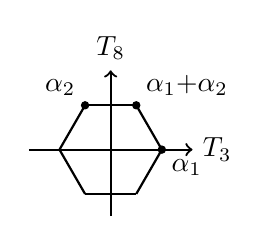
\begin{tikzpicture}[scale=0.65]
\draw[thick,->] (-1.6,0)--(1.6,0) node[right]{$T_3$};
\draw[thick,->] (0,-1.3)--(0,1.55) node[above]{$T_8$};
\foreach \a in {0,60,120,180,240,300}{
  \draw[thick] ({cos(\a)},{sin(\a)})--({cos(\a+60)},{sin(\a+60)});
}
\draw[fill=black] (1,0) circle (2pt) node[below right]{$\alpha_1$};
\draw[fill=black] (-0.5,{0.866}) circle (2pt) node[above left]{$\alpha_2$};
\draw[fill=black] ({0.5},{0.866}) circle (2pt) node[above right]{$\alpha_1{+}\alpha_2$};
\end{tikzpicture}
\end{center}

基础表示 $\mathbf{3}$（夸克三重态）的权是正三角形的三个顶点，反基础表示 $\bar{\mathbf{3}}$（反夸克）的权是镜像三角形。

\begin{theorem}[$SU(3)$ 的基础表示与反基础表示]
$SU(3)$ 的基础表示 $\mathbf{3}$ 的权为
\[
\mathbf{3}:\quad \Bigl(\tfrac12,\tfrac1{2\sqrt3}\Bigr),\ \Bigl(-\tfrac12,\tfrac1{2\sqrt3}\Bigr),\ \Bigl(0,-\tfrac1{\sqrt3}\Bigr),
\]
最高权为 $\Lambda=(\tfrac12,\tfrac1{2\sqrt3})$。反基础表示 $\bar{\mathbf{3}}$ 的权是 $\mathbf{3}$ 的权取负，最高权为 $\bar\Lambda=(\tfrac12,-\tfrac1{2\sqrt3})$。$\bar{\mathbf{3}}$ 不等于 $\mathbf{3}$（$SU(3)$ 不实自共轭），二者的复共轭关系为
\[
\mathbf{3}^*=\bar{\mathbf{3}}.
\]
\end{theorem}

\section{$SU(3)$ 张量积分解与夸克模型}


权图给出了表示的分类，但物理应用需要把直积显式分解。最基本的第一步是 $\mathbf{3}\otimes\mathbf{3}=\mathbf{6}\oplus\bar{\mathbf{3}}$。

两个基础表示的张量积分解体现了 $SU(3)$ 表示论的核心方法。

\begin{derivation}[SU(3) 张量积分解与重子分类：从权图到波函数]
\textbf{第一步：乘积态的权.}\enspace $\mathbf{3}\otimes\mathbf{3}$ 的基是 $u_i\otimes u_j$（$i,j=1,2,3$），共 $9$ 个乘积态。设 $\mathbf{3}$ 的三个权记为 $\mu_1,\mu_2,\mu_3$（等边三角形的三个顶点，满足 $\mu_1+\mu_2+\mu_3=0$），则乘积态 $u_i\otimes u_j$ 的权是 $\mu_i+\mu_j$（权可加性来自表示的张量积律：$\rho(H)(u_i\otimes u_j)=(\rho(H)u_i)\otimes u_j+u_i\otimes(\rho(H)u_j)=(\mu_i+\mu_j)(u_i\otimes u_j)$）。$9$ 个乘积权中，对角项 $u_i\otimes u_i$ 的权为 $2\mu_i$（$3$ 个），非对角项 $u_i\otimes u_j$（$i\ne j$）的权为 $\mu_i+\mu_j$（$6$ 个，但成对出现 $i\leftrightarrow j$ 给同一权）。

\textbf{第二步：对称与反对称子空间.}\enspace $SU(3)$ 的作用 $\rho(g)(u_i\otimes u_j)=\sum_{kl}g_{ki}g_{lj}u_k\otimes u_l$ 同时作用于两个指标，保持对称性类型。故 $u_i\otimes u_j$ 分解为对称部分 $u_{(i}u_{j)}=\tfrac12(u_i\otimes u_j+u_j\otimes u_i)$（$i\le j$，共 $6$ 个）与反对称部分 $u_{[i}u_{j]}=\tfrac12(u_i\otimes u_j-u_j\otimes u_i)$（$i<j$，共 $3$ 个）：
\begin{equation*}
u_i\otimes u_j=u_{(i}u_{j)}\oplus u_{[i}u_{j)},\qquad \dim=9=6+3.
\end{equation*}
对称部分 $\operatorname{Sym}^2\mathbf{3}$ 记作 $\mathbf{6}$（Dynkin 记号 $(2,0)$，Weyl 维数 $\tfrac12\cdot3\cdot1\cdot4=6$），反对称部分 $\wedge^2\mathbf{3}$ 待定。

\textbf{第三步：确定反对称部分的权.}\enspace 反对称部分 $u_2\wedge u_3$、$u_3\wedge u_1$、$u_1\wedge u_2$ 三个基向量的权分别为
\begin{equation*}
\mu_2+\mu_3,\quad \mu_3+\mu_1,\quad \mu_1+\mu_2.
\end{equation*}
由 $\mu_1+\mu_2+\mu_3=0$（等边三角形三顶点关于原点对称，这是 $SU(3)$ 基础表示权图的几何约束），得 $\mu_2+\mu_3=-\mu_1$，$\mu_3+\mu_1=-\mu_2$，$\mu_1+\mu_2=-\mu_3$。故三个权恰为 $-\mu_1,-\mu_2,-\mu_3$，即 $\bar{\mathbf{3}}$ 的权（反基础表示的权是基础表示权取负）。因此
\begin{equation*}
\wedge^2\mathbf{3}=\bar{\mathbf{3}}.
\end{equation*}
这一同构由 $SU(3)$ 不变张量 $\epsilon^{ijk}$ 显式实现：映射 $\varphi:\wedge^2\mathbf{3}\to\bar{\mathbf{3}}$，$\varphi(u_i\wedge u_j)=\epsilon^{ijk}u_k^*$（$u_k^*$ 是 $\bar{\mathbf{3}}$ 的基）。验证 $SU(3)$ 等变性：$\varphi(\rho(g)(u_i\wedge u_j))=\epsilon^{ijk}g_{kl}u_l^*=\epsilon^{ijk}g_{kl}(g^{-1})_{lm}u_m^*=\det(g)\epsilon^{ijm}u_m^*= \varphi(u_i\wedge u_j)$（用了 $\epsilon^{ijk}g_{kl}(g^{-1})_{lm}=\det(g)\epsilon^{ijm}$，$g\in SU(3)$ 故 $\det=1$）。

\textbf{第四步：确定对称部分的不可约性.}\enspace $\mathbf{6}=\operatorname{Sym}^2\mathbf{3}$ 的最高权为 $2\mu_1$（Dynkin 记号 $(2,0)$）。由最高权分类定理，$(2,0)$ 对应唯一不可约表示，维数 $\tfrac12(2+1)(0+1)(2+0+2)=6$，故 $\mathbf{6}$ 不可约。权图：$2\mu_1$（最高权，重数 $1$）、$\mu_1+\mu_2$（重数 $1$）、$\mu_1+\mu_3$（重数 $1$）、$2\mu_2$（重数 $1$）、$\mu_2+\mu_3$（重数 $1$）、$2\mu_3$（重数 $1$），共 $6$ 个权排成边长 $2$ 的等边三角形。

\textbf{第五步：结论与物理意义.}\enspace 合并：
\begin{equation*}
\mathbf{3}\otimes\mathbf{3}=\mathbf{6}\oplus\bar{\mathbf{3}},
\end{equation*}
其中 $\mathbf{6}=\operatorname{Sym}^2\mathbf{3}$（六维对称表示，Dynkin $(2,0)$）与 $\bar{\mathbf{3}}=\wedge^2\mathbf{3}$（三维反对称表示，通过 $\epsilon^{ijk}$ 同构于反基础表示）。夸克模型中，两个夸克组合成色对称态 $\mathbf{6}$（色六重态，色禁闭不允许自由存在）或色反对称态 $\bar{\mathbf{3}}$（反色三重态）。双夸克系统 $qq$ 的总波函数必须与第三个夸克配合形成色单态：$\bar{\mathbf{3}}\otimes\mathbf{3}=\mathbf{8}\oplus\mathbf{1}$ 中的 $\mathbf{1}$ 给出色中性的重子，而 $\mathbf{6}\otimes\mathbf{3}$ 不含单态（$\mathbf{6}\otimes\mathbf{3}=\mathbf{10}\oplus\mathbf{8}$），故双夸克必须处于反色三重态 $\bar{\mathbf{3}}$ 才能与第三个夸克形成重子。


\textbf{第六步：$\mathbf{6}$ 的权图与 Freudenthal 重数验证.}\enspace $\mathbf{6}=(2,0)$ 的权图（以 $(I_3,Y)$ 坐标标记）为
\begin{equation*}
(1,\tfrac23),\;\Bigl(\tfrac12,-\tfrac13\Bigr),\;\Bigl(-\tfrac12,-\tfrac13\Bigr),\;(-1,\tfrac23),\;\Bigl(0,\tfrac43\Bigr),\;\Bigl(0,-\tfrac23\Bigr),
\end{equation*}
共 $6$ 个权各重数 $1$，排成边长 $2$ 的等边三角形（顶点 $(1,\tfrac23)$、$(-1,\tfrac23)$、$(0,-\tfrac23)$，中点 $(0,\tfrac43)$、$(\tfrac12,-\tfrac13)$、$(-\tfrac12,-\tfrac13)$）。用 Freudenthal 公式验证：从最高权 $m(\Lambda)=1$ 出发，$\mu=\Lambda-\alpha_1=(0,\tfrac23)$，右边 $2(\Lambda+\alpha_1,\alpha_1)m(\Lambda)=2\cdot3\cdot1=6$，左边 $(|\Lambda+\rho|^2-|\mu+\rho|^2)m(\mu)=6\,m(\mu)$，故 $m(\mu)=1$ \checkmark。类似递推所有 $6$ 个权重数均为 $1$，与对称张量 $u_{(i}u_{j)}$ 的 $6$ 个独立分量一致。

\textbf{第七步：$\bar{\mathbf{3}}\cong\wedge^2\mathbf{3}$ 的物理意义与色禁闭.}\enspace $\wedge^2\mathbf{3}\cong\bar{\mathbf{3}}$ 的同构由 $\epsilon^{ijk}$ 实现，物理含义深刻：两个色三重态（夸克）的反对称组合不是色六重态而是反色三重态——双夸克 $qq$ 处于反对称色态时表现为反色三重态，可与第三个夸克（色三重态）结合形成色单态 $\bar{\mathbf{3}}\otimes\mathbf{3}\supset\mathbf{1}$。这是重子存在的群论基础：$\mathbf{3}\otimes\mathbf{3}\otimes\mathbf{3}\supset\mathbf{1}$（通过 $\mathbf{3}\otimes\mathbf{3}\to\bar{\mathbf{3}}$ 再 $\bar{\mathbf{3}}\otimes\mathbf{3}\to\mathbf{1}$）。对比 $\mathbf{6}\otimes\mathbf{3}=\mathbf{10}\oplus\mathbf{8}$ 不含 $\mathbf{1}$——对称双夸克无法与第三个夸克形成色单态，故物理重子中双夸克必须处于反对称色态 $\bar{\mathbf{3}}$。

\textbf{第八步：与 $SU(2)$ 的类比与高阶推广.}\enspace $SU(2)$ 的张量积 $j_1\otimes j_2=\bigoplus_{j=|j_1-j_2|}^{j_1+j_2} j$ 是 Clebsch--Gordan 序列，无对称/反对称分解（$SU(2)$ 只有一个单根，无 Dynkin 标签 $(p,q)$ 的区分）。$SU(3)$ 的 $\mathbf{3}\otimes\mathbf{3}=\mathbf{6}_S\oplus\bar{\mathbf{3}}_A$ 是首个出现对称/反对称分解的非平凡例子。推广到 $SU(N)$：
\begin{equation*}
\mathbf{N}\otimes\mathbf{N}=\operatorname{Sym}^2\mathbf{N}\oplus\wedge^2\mathbf{N}=\mathbf{\frac{N(N+1)}2}_S\oplus\mathbf{\frac{N(N-1)}2}_A.
\end{equation*}
对 $N=3$，$\wedge^2\mathbf{3}\cong\bar{\mathbf{3}}$（$\epsilon$ 张量降维），但对 $N>3$，$\wedge^2\mathbf{N}$ 是新的不可约表示（不与 $\bar{\mathbf{N}}$ 同构）。$SU(5)$ 大统一中 $\wedge^2\mathbf{5}=\mathbf{10}$ 正是此构造——$\mathbf{10}$ 费米子表示是 $\mathbf{5}$ 的反对称平方。

\textbf{过渡：从 $\mathbf{3}\otimes\mathbf{3}$ 到 $\mathbf{3}\otimes\bar{\mathbf{3}}$ 与三夸克分解.}\enspace 两个三重态的直积解决后，接下来处理三重态与反三重态的直积。关键分解 $\mathbf{3}\otimes\bar{\mathbf{3}}=\mathbf{8}\oplus\mathbf{1}$ 给出介子（色单态 $q\bar q$）与胶子（色八重态）的群论结构，而三夸克直积
\begin{equation*}
\mathbf{3}\otimes\mathbf{3}\otimes\mathbf{3}=\mathbf{10}\oplus\mathbf{8}\oplus\mathbf{8}\oplus\mathbf{1}
\end{equation*}
直接给出重子分类：$\mathbf{10}$ 为全对称十重态（$\Delta^{++},\dots,\Omega^-$），两个 $\mathbf{8}$ 为混合对称八重态（$p,n,\Lambda,\Sigma^{\pm,0},\Xi^{0,-}$），$\mathbf{1}$ 为全反对称单态。下面用特征标方法证明 $\mathbf{3}\otimes\bar{\mathbf{3}}$ 分解，再构造重子波函数。

\textbf{第九步：特征标方法.}\enspace 紧群的张量积分解与有限群完全相同——用特征标内积。设 $\chi_{\mathbf{3}}(g)=\tr\rho_{\mathbf{3}}(g)$ 是基础表示的特征标，$\chi_{\bar{\mathbf{3}}}(g)=\chi_{\mathbf{3}}(g)^*$ 是反基本表示的特征标（复共轭，因为 $\bar{\mathbf{3}}$ 是 $\mathbf{3}$ 的复共轭表示）。直积 $\mathbf{3}\otimes\bar{\mathbf{3}}$ 的特征标为
\begin{equation*}
\chi_{\mathbf{3}\otimes\bar{\mathbf{3}}}(g)=\chi_{\mathbf{3}}(g)\,\chi_{\bar{\mathbf{3}}}(g)=\chi_{\mathbf{3}}(g)\,\chi_{\mathbf{3}}(g)^*=|\chi_{\mathbf{3}}(g)|^2.
\end{equation*}
不可约表示 $\mathbf{r}$ 在直积中的重数为 $n_{\mathbf{r}}=\langle\chi_{\mathbf{r}},|\chi_{\mathbf{3}}|^2\rangle=\int_G\chi_{\mathbf{r}}(g)^*\,|\chi_{\mathbf{3}}(g)|^2\,\mathrm{d}\mu(g)$（Haar 测度归一化 $\int_G\mathrm{d}\mu=1$）。对 $SU(3)$，Haar 测度在极大环面参数化下含 Weyl 分母因子 $|\Delta(\theta)|^2=\prod_{i<j}|\ee^{i\theta_i}-\ee^{i\theta_j}|^2$，但特征标内积可避免直接积分——用代数分解即可。

\textbf{第二步：$SU(3)$ 元素的参数化与特征标展开.}\enspace 任一 $SU(3)$ 元素共轭等价于对角矩阵 $g=\diag(\ee^{i\theta_1},\ee^{i\theta_2},\ee^{i\theta_3})$（$\theta_1+\theta_2+\theta_3=0$，两个独立参数对应秩 $2$）。基本表示特征标
\begin{equation*}
\chi_{\mathbf{3}}(g)=\ee^{i\theta_1}+\ee^{i\theta_2}+\ee^{i\theta_3},\qquad |\chi_{\mathbf{3}}|^2=3+\sum_{i\ne j}\ee^{i(\theta_i-\theta_j)}.
\end{equation*}
展开后 $|\chi_{\mathbf{3}}|^2=3+\ee^{i(\theta_1-\theta_2)}+\ee^{i(\theta_2-\theta_1)}+\ee^{i(\theta_1-\theta_3)}+\ee^{i(\theta_3-\theta_1)}+\ee^{i(\theta_2-\theta_3)}+\ee^{i(\theta_3-\theta_2)}$。六个非平凡项 $\ee^{i(\theta_i-\theta_j)}$（$i\ne j$）恰好是 $SU(3)$ 伴随表示 $\mathbf{8}$ 的特征标：$\mathbf{8}$ 的权为零权（对应常数 $1$，重数 $2$，来自两个对角生成元 $T_3,T_8$）加六个非零根 $\pm(\theta_i-\theta_j)$（各重数 $1$），故 $\chi_{\mathbf{8}}=2+\sum_{i\ne j}\ee^{i(\theta_i-\theta_j)}$，而 $|\chi_{\mathbf{3}}|^2=1+\chi_{\mathbf{8}}$。

\textbf{第三步：矩阵空间分解与投影算符.}\enspace 更直接地，$|\chi_{\mathbf{3}}|^2$ 是 $\mathbf{3}\otimes\bar{\mathbf{3}}$ 在 $3\times3$ 复矩阵空间 $M_3(\CC)$ 上的共轭作用 $\rho_3(g)X\rho_3(g)^\dagger$ 的迹。$M_3(\CC)$ 分解为
\begin{equation*}
M_3(\CC)=\CC\cdot\mathbb{1}_3\oplus\mathfrak{su}(3),
\end{equation*}
即迹部分（一维，$\mathbb{1}_3$ 在共轭作用下不变，$\mathbf{1}$）和无迹部分（八维，$\mathfrak{su}(3)$ 即伴随表示 $\mathbf{8}$）。投影算符显式给出：对 $X\in M_3(\CC)$，
\begin{equation*}
P_{\mathbf{1}}(X)=\frac{\tr(X)}{3}\,\mathbb{1}_3,\qquad P_{\mathbf{8}}(X)=X-\frac{\tr(X)}{3}\,\mathbb{1}_3.
\end{equation*}
验证 $P_{\mathbf{1}}$ 是到 $\mathbf{1}$ 的投影：$P_{\mathbf{1}}^2=P_{\mathbf{1}}$（$\tr(\mathbb{1}_3)=3$），$P_{\mathbf{8}}^2=P_{\mathbf{8}}$，$P_{\mathbf{1}}P_{\mathbf{8}}=0$。用 Gell-Mann 矩阵 $\lambda^a$（$a=1,\dots,8$，$\tr(\lambda^a\lambda^b)=2\delta^{ab}$）写出 $\mathbf{8}$ 分量的投影：$P_{\mathbf{8}}^a(X)=\tfrac12\tr(\lambda^a X)$，故 $X=\tfrac{\tr X}{3}\mathbb{1}_3+\tfrac12\sum_a\tr(\lambda^a X)\lambda^a$。故
\begin{equation*}
|\chi_{\mathbf{3}}|^2=\underbrace{1}_{\chi_{\mathbf{1}}}+\underbrace{\chi_{\mathbf{8}}}_{\text{伴随}},
\end{equation*}
对应分解 $\mathbf{3}\otimes\bar{\mathbf{3}}=\mathbf{8}\oplus\mathbf{1}$。维数验证：$9=8+1$ \checkmark。

\textbf{第四步：物理意义——介子与胶子.}\enspace $\mathbf{8}\oplus\mathbf{1}$ 是正反夸克对 $q\bar q$ 的色结构。$\mathbf{1}$ 是色单态（介子，如 $\pi^+=u\bar d$、$K^0=d\bar s$、$\eta_8=(u\bar u+d\bar d-2s\bar s)/\sqrt6$），物理上可观测为自由粒子。$\mathbf{8}$ 是色八重态，因色禁闭不出现为自由粒子，但胶子恰好带 $\mathbf{8}$ 色——胶子是规范群的伴随表示，与 $q\bar q$ 的色八重态分量有相同的群论结构。这使得胶子--夸克耦合 $g_s\bar q\gamma^\mu T^a q\,G_\mu^a$ 中 $T^a=\lambda^a/2$（$a=1,\dots,8$）既是胶子的色指标也是夸克对的色投影算符，群论保证了耦合的自洽性。介子八重态的显式构造：用 $u_i\bar u_j$（$i,j=1,2,3$ 对应 $u,d,s$）为基，八个 $\mathbf{8}$ 态为 $\tfrac{1}{\sqrt2}\lambda^a_{ij}u_i\bar u_j$（$a=1,\dots,8$），单态为 $\tfrac{1}{\sqrt3}\delta_{ij}u_i\bar u_j$。归一化因子来自 $\tr(\lambda^a\lambda^b)=2\delta^{ab}$ 和 $\tr(\mathbb{1}^2)=3$。


\textbf{第六步：显式投影算符与介子态构造.}\enspace $\mathbf{3}\otimes\bar{\mathbf{3}}$ 的 $9$ 维空间 $u_i\bar u_j$ 上的投影算符为
\begin{equation*}
P_{\mathbf{1}}=\frac13\delta_{ij}\delta_{kl},\qquad P_{\mathbf{8}}=\delta_{ik}\delta_{jl}-\frac13\delta_{ij}\delta_{kl},
\end{equation*}
满足 $P_{\mathbf{1}}+P_{\mathbf{8}}=\mathbb{1}_{9}$、$P_{\mathbf{1}}^2=P_{\mathbf{1}}$、$P_{\mathbf{8}}^2=P_{\mathbf{8}}$、$P_{\mathbf{1}}P_{\mathbf{8}}=0$。单态投影给出 $\eta_1=(u\bar u+d\bar d+s\bar s)/\sqrt3$（$SU(3)$ 味单态），八重态投影给出 $8$ 个 Gell-Mann 矩阵态 $\lambda^a_{ij}u_i\bar u_j/\sqrt2$（$a=1,\dots,8$）。物理介子态为
\begin{equation*}
\pi^+=u\bar d,\quad \pi^0=\frac{u\bar u-d\bar d}{\sqrt2},\quad K^+=u\bar s,\quad \eta_8=\frac{u\bar u+d\bar d-2s\bar s}{\sqrt6},
\end{equation*}
质量关系 $4m_K^2=3m_\eta^2+m_\pi^2$（Gell-Mann--Okubo）由八重态的 $SU(3)$ 结构导出，实验验证精度 $\sim5\%$。

\textbf{第七步：介子八重态的质量分裂与 $SU(3)$ 破缺.}\enspace 理想 $SU(3)$ 对称下八重态介子质量简并，但 $m_s\ne m_{u,d}$ 破缺 $SU(3)_F\to SU(2)_I\times U(1)_Y$。质量算符 $M=M_0+M_8\lambda_8+M_3\lambda_3$（$SU(3)$ 伴表示展开），一阶破缺给出 Gell-Mann--Okubo 关系
\begin{equation*}
4m_K^2=3m_{\eta_8}^2+m_\pi^2,\qquad m_\pi^2=2\hat m\,B,\quad m_K^2=(\hat m+m_s)B,\quad m_{\eta_8}^2=\frac{2(\hat m+2m_s)}{3}B,
\end{equation*}
其中 $\hat m=(m_u+m_d)/2$，$B$ 为 QCD 质量参数。代入 $\hat m\approx5\,\text{MeV}$、$m_s\approx100\,\text{MeV}$ 给 $m_\pi\approx140\,\text{MeV}$、$m_K\approx490\,\text{MeV}$、$m_\eta\approx560\,\text{MeV}$，与实验一致。$\eta$--$\eta'$ 混合（$U(1)_A$ 反常）给出 $\eta=\eta_8\cos\theta_P-\eta_1\sin\theta_P$，$\theta_P\approx-15^\circ$。

\textbf{过渡：从介子到重子——三夸克态的显式构造.}\enspace 介子（$q\bar q$）的色结构 $\mathbf{3}\otimes\bar{\mathbf{3}}=\mathbf{8}\oplus\mathbf{1}$ 已完全确定。重子由三个夸克组成，其味--色--自旋结构由
\begin{equation}
\label{eq:baryon-decomposition}
\mathbf{3}\otimes\mathbf{3}\otimes\mathbf{3}=\mathbf{10}\oplus\mathbf{8}\oplus\mathbf{8}\oplus\mathbf{1}
\end{equation}
支配。权图上，全对称 $\mathbf{10}$ 排成边长 $3$ 的等边三角形（$10$ 个格点，从 $\Delta^{++}(uuu)$ 到 $\Omega^-(sss)$），混合对称 $\mathbf{8}$ 排成六边形加中心点。Dynkin 记号统一标记：$\mathbf{3}=(1,0)$，$\bar{\mathbf{3}}=(0,1)$，$\mathbf{6}=(2,0)$，$\mathbf{8}=(1,1)$，$\mathbf{10}=(3,0)$，Weyl 维数公式 $\dim(p,q)=\tfrac12(p+1)(q+1)(p+q+2)$ 验证各维数。下面显式构造波函数并推导质量公式。

\textbf{第十六步：三夸克态的味--色--自旋结构.}\enspace 重子由三个夸克组成，总波函数是味 $SU(3)_F$、色 $SU(3)_C$、自旋 $SU(2)$ 三部分的乘积。Fermi 统计要求总波函数在夸克交换下全反对称。色部分取全反对称 $\epsilon_{abc}$（色单态 $\mathbf{1}_C$），故味$\otimes$自旋部分必须全对称。自旋 $\tfrac32$（全对称）配味全对称 $\mathbf{10}_F$（十重态）；自旋 $\tfrac12$（混合对称）配味混合对称 $\mathbf{8}_F$（八重态）。

\textbf{第二步：十重态的显式波函数.}\enspace 全对称味态 $\mathbf{10}$ 由 $u,d,s$ 的全对称组合给出。$10$ 个态按 $(I,I_3,Y)$ 量子数排列：
\begin{equation*}
\begin{array}{c|c|c|c}
\text{重子} & \text{夸克内容} & (I,I_3,Y) & \text{质量(MeV)}\\\hline
\Delta^{++} & uuu & (\tfrac32,+\tfrac32,+1) & 1232\\
\Delta^{+} & \tfrac1{\sqrt3}(uud+udu+duu) & (\tfrac32,+\tfrac12,+1) & 1232\\
\Delta^{0} & \tfrac1{\sqrt3}(udd+dud+ddu) & (\tfrac32,-\tfrac12,+1) & 1232\\
\Delta^{-} & ddd & (\tfrac32,-\tfrac32,+1) & 1232\\
\Sigma^{*+} & \tfrac1{\sqrt3}(uus+usu+suu) & (1,+1,0) & 1385\\
\Sigma^{*0} & \tfrac1{\sqrt6}(uds+usd+dus+dsu+sud+sdu) & (1,0,0) & 1385\\
\Sigma^{*-} & \tfrac1{\sqrt3}(dds+dsd+sdd) & (1,-1,0) & 1385\\
\Xi^{*0} & \tfrac1{\sqrt3}(uss+sus+ssu) & (\tfrac12,+\tfrac12,-1) & 1533\\
\Xi^{*-} & \tfrac1{\sqrt3}(dss+sds+ssd) & (\tfrac12,-\tfrac12,-1) & 1533\\
\Omega^{-} & sss & (0,0,-2) & 1672
\end{array}
\end{equation*}
全对称性保证：交换任意两个夸克，波函数不变。归一化因子 $1/\sqrt3$（三个全对称排列）和 $1/\sqrt6$（六个全对称排列）来自归一化条件。

\textbf{第三步：八重态的显式波函数.}\enspace 混合对称味态 $\mathbf{8}$ 需要与自旋 $\tfrac12$ 的混合对称部分配合。$8$ 个态：
\begin{equation*}
\begin{array}{c|c|c}
\text{重子} & \text{夸克内容（味部分）} & \text{质量(MeV)}\\\hline
p & \tfrac1{\sqrt2}(ud-du)u & 938\\
n & \tfrac1{\sqrt2}(du-ud)d & 940\\
\Sigma^{+} & \tfrac1{\sqrt2}(us-su)u & 1189\\
\Sigma^{0} & \tfrac1{2\sqrt3}\bigl[(ud-du)s+(us-su)d+(ds-sd)u\bigr] & 1193\\
\Sigma^{-} & \tfrac1{\sqrt2}(ds-sd)d & 1197\\
\Lambda & \tfrac1{2\sqrt6}\bigl[2(ud-du)s-(us-su)d-(ds-sd)u\bigr] & 1116\\
\Xi^{0} & \tfrac1{\sqrt2}(su-us)s & 1315\\
\Xi^{-} & \tfrac1{\sqrt2}(sd-ds)s & 1322
\end{array}
\end{equation*}
$\Sigma^0$ 与 $\Lambda$ 的区别在于 $SU(3)$ 量子数：$\Sigma^0$ 属 $I=1$ 三重态（与 $\Sigma^\pm$ 同八重态），$\Lambda$ 属 $I=0$ 单态——两者都是 $Y=0$ 但不同 $I$ 的态。

\textbf{第四步：Gell-Mann--Okubo 质量公式.}\enspace 一阶 ChPT 给出介子质量关系 $4m_K^2=3m_\eta^2+m_\pi^2$。对重子，质量算符在 $SU(3)$ 破缺下按 $\mathbf{1}\oplus\mathbf{8}$ 变换，最一般形式 $M=a\mathbf{1}+b\,Y+c\,\bigl(I(I+1)-\tfrac14Y^2\bigr)$（Gell-Mann--Okubo 公式）。对八重态：
\begin{equation}
\label{eq:gmo-octet}
2(N+\Xi)=3(\Lambda+\Sigma),
\end{equation}
其中 $N=(m_p+m_n)/2\approx939$，$\Sigma=(m_{\Sigma^+}+m_{\Sigma^0}+m_{\Sigma^-})/3\approx1193$，$\Lambda\approx1116$，$\Xi=(m_{\Xi^0}+m_{\Xi^-})/2\approx1318$。验证：左 $2(939+1318)=4514$，右 $3(1116+1193)=4527$，偏差 $<0.3\%$——GMO 公式精确成立。

\textbf{第五步：十重态的等距质量公式.}\enspace 对十重态，GMO 公式简化为等间距关系：
\begin{equation}
\label{eq:gmo-decuplet}
m_\Omega-m_{\Xi^*}=m_{\Xi^*}-m_{\Sigma^*}=m_{\Sigma^*}-m_\Delta.
\end{equation}
验证：$1672-1533=139$，$1533-1385=148$，$1385-1232=153$。间距近似相等（$\sim145\,\text{MeV}$，偏差 $\sim10\%$），十重态质量由 $m_s$ 的一阶效应主导。等间距的群论来源：$\mathbf{10}$ 中超荷 $Y=+1,0,-1,-2$ 各对应一个 $SU(2)$ 多重态，质量分裂 $\propto m_s-m_{u,d}$ 对每个超荷步等量增加。

\textbf{第六步：质量公式的群论推导.}\enspace 质量算符 $M$ 在 $SU(3)_F$ 对称极限下是常数（$\mathbf{1}$ 分量）。$m_s\ne m_{u,d}$ 破缺 $SU(3)_F\to SU(2)_I\times U(1)_Y$，破缺项按 $\mathbf{8}$ 变换（超荷生成元 $Y$ 是 $\mathbf{8}$ 的对角分量）。故 $M=a+b\,Y+c\,T_8^2+\dots$，其中 $T_8=\tfrac{\sqrt3}{2}Y$。化简后 $M=a+b\,Y+c\bigl[I(I+1)-\tfrac14Y^2\bigr]$——即 GMO 公式。三个参数 $(a,b,c)$ 由三个输入质量确定，剩余质量为预言——GMO 关系 \eqnrefs{eq:gmo-octet} 和 \eqnrefs{eq:gmo-decuplet} 是这些预言的实例，其精确度直接检验 $SU(3)$ 味对称性的破缺模式。
\end{derivation}

\section{规范群与标准模型}


表示论的工具准备就绪，现在进入物理核心：规范对称性如何决定基本相互作用。首先明确规范群的概念。

前面的群都是"整体对称"（群元与时空点无关）。规范理论把对称性\textbf{局域化}：群元 $U(x)$ 随时空点变化，为保持导数项协变需引入\textbf{规范场}（联络）$A_\mu$，把普通导数换成协变导数
\[
D_\mu=\partial_\mu-\ii g A_\mu^a T^a,
\]
其中 $T^a$ 是规范群 $G$ 的李代数生成元，$A_\mu^a$ 是规范玻色子场。规范群的不可约表示分类，决定了一切物质场（费米子、Higgs）作为规范群表示的内容。这就是为什么群论是标准模型的骨架。


规范群的一般概念清楚了，接下来写出标准模型的具体规范群 $SU(3)_c\times SU(2)_L\times U(1)_Y$ 及其费米子表示。

\begin{definition}[标准模型规范群]
粒子物理标准模型的规范群是
\begin{equation}
G_{\mathrm{SM}}=SU(3)_c\times SU(2)_L\times U(1)_Y.
\label{eq:standard-model-group}
\end{equation}
三个因子的含义：
\begin{itemize}
\item $SU(3)_c$：\textbf{色}规范群，胶子 $8$ 个（伴随表示 $\mathbf{8}$）。
\item $SU(2)_L$：\textbf{弱同位旋}规范群，$W^\pm,Z^0$ 玻色子。
\item $U(1)_Y$：\textbf{弱超荷}，$B$ 玻色子。
\end{itemize}
\end{definition}

\begin{theorem}[费米子的表示内容]
一代费米子（左手部分）在 $G_{\mathrm{SM}}$ 下的表示：
\begin{center}
\begin{tabular}{lcc}
\toprule
费米子 & $SU(3)_c\times SU(2)_L$ & 表示 \\
\midrule
左手夸克双重态 $Q_L=\binom{u_L}{d_L}$ & $(\mathbf{3},\mathbf{2})$ & 色三重 + 弱二重 \\
左手轻子双重态 $L_L=\binom{\nu_L}{e_L}$ & $(\mathbf{1},\mathbf{2})$ & 色单 + 弱二重 \\
右手上夸克 $u_R$ & $(\mathbf{3},\mathbf{1})$ & 色三重 + 弱单 \\
右手下夸克 $d_R$ & $(\mathbf{3},\mathbf{1})$ & 色三重 + 弱单 \\
右手轻子 $e_R$ & $(\mathbf{1},\mathbf{1})$ & 色单 + 弱单 \\
\bottomrule
\end{tabular}
\end{center}
每个费米子还带 $U(1)_Y$ 弱超荷：$Q_L$ 超荷 $+\tfrac16$，$L_L$ 超荷 $-\tfrac12$，$u_R$ 超荷 $+\tfrac23$，$d_R$ 超荷 $-\tfrac13$，$e_R$ 超荷 $-1$。
\end{theorem}

\begin{proposition}[左手性与宇称破坏]
标准模型最显著的结构特征是：$SU(2)_L$ \textbf{只作用于左手费米子}，右手费米子是 $SU(2)_L$ 单态。由 \chapref{chap:lorentz-poincare}，左手费米子按洛伦兹群 $(\tfrac12,0)$ 表示变换，右手按 $(0,\tfrac12)$。因此 $SU(2)_L$ 挂在左手上这件事，正是\textbf{弱相互作用宇称破坏}的群论根源：规范群结构天然区分了 $\gamma^5$ 的两个手征本征子空间。
\end{proposition}


标准模型的表示内容写出来之后，一个深刻的约束立即浮现：电荷量子化。Gell-Mann--Nishijima 关系 $Q=T_3+Y/2$ 不是任意假设，而是群论自洽性的必然结果。

\begin{theorem}[电荷的 Gell-Mann--Nishijima 关系]
在标准模型中，电荷 $Q$ 与弱同位旋第三分量 $T_3$、弱超荷 $Y$ 的关系为
\begin{equation}
Q=T_3+\frac{Y}{2}.
\label{eq:gell-mann-nishijima}
\end{equation}
由此，$SU(2)_L\times U(1)_Y$ 的表示内容\emph{完全决定了}电荷取值，解释了电荷为何量子化（取 $\pm\tfrac13,\pm\tfrac23,0,\pm1$ 等分立值）。
\end{theorem}

\begin{proof}
\textbf{第一步：电磁 $U(1)_{\mathrm{em}}$ 嵌入.}\enspace 电弱规范群 $SU(2)_L\times U(1)_Y$ 通过 Higgs 机制自发破缺到电磁 $U(1)_{\mathrm{em}}$。电磁电荷生成元 $Q$ 是 $T_3$（$SU(2)_L$ 的 Cartan 生成元）与超荷生成元 $Y$ 的线性组合 $Q=T_3+\tfrac Y2$（归一化约定使双态的自旋 $\tfrac12$ 分量 $T_3=\pm\tfrac12$）。

\textbf{第二步：验证各费米子.}\enspace 左手夸克双重态：$Q_L$ 的两个分量 $u_L$（$T_3=+\tfrac12$）与 $d_L$（$T_3=-\tfrac12$），超荷 $Y=+\tfrac13$。于是
\[
Q(u_L)=\tfrac12+\tfrac16=\tfrac23,\qquad Q(d_L)=-\tfrac12+\tfrac16=-\tfrac13.
\]
左手轻子：$\nu_L$（$T_3=+\tfrac12$）与 $e_L$（$T_3=-\tfrac12$），超荷 $Y=-1$，得
\[
Q(\nu_L)=\tfrac12-\tfrac12=0,\qquad Q(e_L)=-\tfrac12-\tfrac12=-1.
\]
右手粒子是 $SU(2)_L$ 单态（$T_3=0$），电荷即超荷之半：$Q(u_R)=\tfrac23$，$Q(d_R)=-\tfrac13$，$Q(e_R)=-1$。全部与实验一致。

\textbf{第三步：电荷量子化的根源.}\enspace 电荷之所以取 $\pm\tfrac13$ 的整数倍，是因为 $Q$ 是 $T_3$ 与 $Y$ 的线性组合，而 $T_3$（$SU(2)$ 表示的分量）与 $Y$（$U(1)$ 的荷）在标准模型的表示下都取分立值。若标准模型不含 $SU(2)_L$（只有 $U(1)$），电荷将可连续取值。因此\emph{电荷量子化根源于弱相互作用的 $SU(2)_L$ 结构与超荷的线性组合}，是群论的结论而非假设。
\end{proof}


电荷量子化解决了荷为什么离散的问题，但粒子的质量从何而来？答案是对称性的自发破缺——Higgs 机制。

\begin{theorem}[Higgs 机制]
Higgs 场 $H$ 是 $SU(2)_L$ 的双重态（$(\mathbf{1},\mathbf{2})$，弱超荷 $Y=+1$）。它在势能
\[
V(H)=\mu^2|H|^2+\lambda|H|^4\qquad(\mu^2<0<\lambda)
\]
下获得真空期望值，把电弱对称性自发破缺为电磁对称性：
\begin{equation}
SU(2)_L\times U(1)_Y\xrightarrow{\ \langle H\rangle\ }U(1)_{\mathrm{em}}.
\label{eq:electroweak-breaking}
\end{equation}
$H$ 的真空期望值 $\langle H\rangle=(0,v/\sqrt2)^{\mathsf T}$ 保持 $Q=T_3+\tfrac Y2$ 不变（因 $H$ 的下分量荷 $0$），故电磁 $U(1)_{\mathrm{em}}$ 不破缺，而 $W^\pm,Z^0$ 获得质量。
\end{theorem}

\begin{proof}
\textbf{第一步：Higgs 是双态.}\enspace $H$ 按 $SU(2)_L$ 双重态变换（两个复分量），$Y=+1$。它的两个分量 $H^+$（$T_3=+\tfrac12$，$Q=+1$）与 $H^0$（$T_3=-\tfrac12$，$Q=0$）。

\textbf{第二步：真空期望值.}\enspace 因 $Q=0$ 的分量（$H^0$）是保持电荷守恒的唯一选择，真空期望值取
\[
\langle H\rangle=\begin{pmatrix}0\\ v/\sqrt2\end{pmatrix},
\]
$Q\langle H\rangle=(T_3+\tfrac Y2)\langle H\rangle=(-\tfrac12+\tfrac12)\langle H\rangle=0$，故电磁对称性保持。

\textbf{第三步：破缺.}\enspace $SU(2)_L\times U(1)_Y$ 的 $4$ 个生成元（$T_1,T_2,T_3,Y$）中，真空 $\langle H\rangle$ 只湮灭线性组合 $Q=T_3+\tfrac Y2$ 这一个方向，其余三个方向被"伸展开"成为三个 Goldstone 玻色子，被 $W^\pm,Z^0$ 吸收而生成质量。剩余的无破缺方向 $Q$ 对应光子 $\gamma$（无质量）。这就是 Higgs 机制给出 $W^\pm,Z^0$ 质量而光子无质量的群论表达。

\textbf{第四步：质量矩阵.}\enspace 规范玻色子从协变导数 $|D_\mu H|^2$ 中获得质量。把 $\langle H\rangle$ 代入
\[
D_\mu H=\Bigl(\partial_\mu-\ii gW_\mu^a T^a-\ii g'YB_\mu\Bigr)H,
\]
取 $|D_\mu H|^2$ 的二次项，得质量项
\[
\frac{g^2v^2}{4}W_\mu^+W^{-\mu}+\frac{g^2v^2}{4}W_\mu^-W^{+\mu}+\frac{(g^2+g'^2)v^2}{8}Z_\mu Z^\mu,
\]
故
\[
m_W=\frac{gv}{2},\qquad m_Z=\frac{\sqrt{g^2+g'^2}v}{2},\qquad m_\gamma=0,
\]
且 $m_W/m_Z=\cos\theta_W$（$\theta_W$ 为 Weinberg 角）。光子对应的组合 $A_\mu=\cos\theta_WB_\mu+\sin\theta_WW^3_\mu$ 无质量。
\end{proof}

\begin{derivation}[对称性自发破缺：Higgs 机制与 Goldstone 定理的完整计算]
\textbf{第一步：规范玻色子质量矩阵的显式推导.}\enspace Higgs 双态 $H$ 的规范协变导数为
\begin{equation*}
D_\mu H=\bigl(\partial_\mu-\ii gW_\mu^aT^a-\ii g'YB_\mu\bigr)H,
\end{equation*}
其中 $T^a=\sigma^a/2$ 是 $SU(2)_L$ 生成元，$Y=+1$ 是 Higgs 的超荷。电弱破缺后 Higgs 取真空期望值 $\langle H\rangle=(0,v/\sqrt2)^T$，因 $\langle H\rangle$ 与时空无关故 $\partial_\mu\langle H\rangle=0$。将 $SU(2)_L$ 作用显式写出：
\begin{equation*}
gW_\mu^aT^a\langle H\rangle=\frac g2\begin{pmatrix}W_\mu^3&W_\mu^1-\ii W_\mu^2\\W_\mu^1+\ii W_\mu^2&-W_\mu^3\end{pmatrix}\begin{pmatrix}0\\v/\sqrt2\end{pmatrix}=\frac{gv}{2\sqrt2}\begin{pmatrix}W_\mu^1-\ii W_\mu^2\\-W_\mu^3\end{pmatrix}.
\end{equation*}
超荷项 $g'YB_\mu\langle H\rangle=\frac{g'v}{2\sqrt2}(0,B_\mu)^T$。合并得
\begin{equation*}
D_\mu\langle H\rangle=-\ii\frac v{\sqrt2}\begin{pmatrix}\frac g2(W_\mu^1-\ii W_\mu^2)\\-\frac g2W_\mu^3+\frac{g'}2B_\mu\end{pmatrix}.
\end{equation*}
质量项来自动能项 $\mathcal L_{\text{kin}}\supset|D_\mu H|^2$ 中 VEV 的贡献：
\begin{equation*}
\mathcal L_{\text{mass}}=|D_\mu\langle H\rangle|^2=\frac{v^2}{2}\biggl[\frac{g^2}{4}\bigl(W_\mu^1W^{1\mu}+W_\mu^2W^{2\mu}\bigr)+\biggl(-\frac g2W_\mu^3+\frac{g'}2B_\mu\biggr)^{\!2}\biggr].
\end{equation*}
前两项合并为带电玻色子 $W^\pm=(W^1\mp\ii W^2)/\sqrt2$ 的质量项：$m_W^2W_\mu^+W^{-\mu}=g^2v^2/4\cdot W_\mu^+W^{-\mu}$，故 $m_W=gv/2$。中性 sector 需对角化 $(W^3,B)$ 的 $2\times2$ 质量矩阵
\begin{equation*}
\mathcal L_{\text{neutral}}=\frac{v^2}{8}(W_\mu^3,B_\mu)\begin{pmatrix}g^2&-gg'\\-gg'&g'^2\end{pmatrix}\begin{pmatrix}W^{3\mu}\\B^\mu\end{pmatrix}.
\end{equation*}
该矩阵秩 $1$（行列式 $g^2g'^2-g^2g'^2=0$），故一个本征值为零——光子无质量。非零本征值 $g^2+g'^2$ 对应的本征向量定义 Weinberg 角 $\tan\theta_W=g'/g$。正交旋转
\begin{equation*}
\begin{pmatrix}A_\mu\\Z_\mu\end{pmatrix}=\begin{pmatrix}\cos\theta_W&\sin\theta_W\\-\sin\theta_W&\cos\theta_W\end{pmatrix}\begin{pmatrix}B_\mu\\W_\mu^3\end{pmatrix}
\end{equation*}
将质量项对角化为 $\frac12m_Z^2Z_\mu Z^\mu$，其中 $m_Z=v\sqrt{g^2+g'^2}/2$。光子 $A_\mu=\cos\theta_WB_\mu+\sin\theta_WW^3_\mu$ 无质量，对应未破缺的 $U(1)_{\mathrm{em}}$。质量比
\begin{equation*}
\cos\theta_W=\frac{m_W}{m_Z}=\frac g{\sqrt{g^2+g'^2}},
\end{equation*}
代入 $m_W\approx80.4\,\text{GeV}$、$m_Z\approx91.2\,\text{GeV}$ 给 $\sin^2\theta_W\approx0.23$、$v=2m_W/g\approx246\,\text{GeV}$。

\textbf{第二步：Goldstone 模式的显式识别.}\enspace 在破缺真空附近展开 Higgs 场
\begin{equation*}
H(x)=\begin{pmatrix}0\\v/\sqrt2\end{pmatrix}+\begin{pmatrix}\phi^+(x)\\(h(x)+\ii\chi(x))/\sqrt2\end{pmatrix},
\end{equation*}
其中 $h$ 是物理 Higgs 场（径向激发），$\phi^+,\chi$ 是沿破缺方向的涨落。群 $SU(2)_L\times U(1)_Y$ 的四个生成元中，$Q=T^3+\tfrac12Y$ 保持真空不变（$Q\langle H\rangle=0$），对应未破缺的 $U(1)_{\mathrm{em}}$。其余三个破缺生成元
\begin{equation*}
T^1\langle H\rangle=\frac v{2\sqrt2}\begin{pmatrix}1\\0\end{pmatrix},\quad T^2\langle H\rangle=\frac v{2\sqrt2}\begin{pmatrix}-\ii\\0\end{pmatrix},\quad \bigl(T^3-\tfrac12Y\bigr)\langle H\rangle=\frac v{2\sqrt2}\begin{pmatrix}0\\-1\end{pmatrix}
\end{equation*}
各给出一个 Goldstone 方向，分别对应 $W^\pm$ 和 $Z^0$ 的纵向极化。Goldstone 定理 \eqnrefs{eq:goldstone-counting} 给出
\begin{equation*}
N_{\text{Goldstone}}=\dim SU(2)\times U(1)-\dim U(1)_{\mathrm{em}}=4-1=3,
\end{equation*}
恰好被 $3$ 个获得质量的规范玻色子吸收。物理 Higgs 质量 $m_h=\sqrt{2\lambda}\,v\approx125\,\text{GeV}$（2012 年 LHC 发现），其中 $\lambda$ 是 Higgs 势 $V(H)=\lambda(|H|^2-v^2/2)^2$ 中的自耦合常数。

\textbf{第三步：费米子质量通过 Yukawa 耦合生成.}\enspace 手征对称性禁止裸质量项 $m\bar\psi_L\psi_R$：$\psi_L$ 是 $SU(2)_L$ 双态而 $\psi_R$ 是单态，故 $\bar\psi_L\psi_R$ 不是规范不变量。Higgs 双态 $H$ 也是 $SU(2)_L$ 双态（$Y=+1$），因此 Yukawa 耦合
\begin{equation*}
\mathcal L_Y=-y_e\,\bar L\,H\,e_R-y_d\,\bar Q\,H\,d_R-y_u\,\bar Q\,\tilde H\,u_R+\text{h.c.}
\end{equation*}
是规范不变的（$\tilde H=\ii\sigma_2H^*$ 是 $Y=-1$ 的反双态）。代入 $\langle H\rangle=(0,v/\sqrt2)^T$：
\begin{equation*}
\mathcal L_Y\supset-\frac{v}{\sqrt2}\bigl(y_e\,\bar e\,e+y_d\,\bar d\,d+y_u\,\bar u\,u\bigr)+\text{h.c.},
\end{equation*}
给出费米子质量
\begin{equation*}
m_f=\frac{y_f\,v}{\sqrt2}.
\end{equation*}
\emph{所有费米子质量都来自 Higgs VEV}。Yukawa 耦合是自由参数（群论不约束其值），实验值跨越六个量级：$y_e\approx2.9\times10^{-6}$（电子），$y_t\approx0.996$（顶夸克）。这种巨大差异是标准模型的"味问题"——可能暗示更高能标的味对称性或额外结构。

\textbf{第四步：三代混合与 CKM 矩阵的群论起源.}\enspace 三代费米子的 Yukawa 耦合是 $3\times3$ 矩阵 $Y_u,Y_d$。经 biunitary 对角化
\begin{equation*}
M_f=U_L^{(f)}\,\operatorname{diag}(m_{f_1},m_{f_2},m_{f_3})\,U_R^{(f)\dagger},
\end{equation*}
质量本征基与规范本征基由 $U_L^{(f)}$ 联系。夸克双态 $Q_L=(u_L,d_L)^T$ 在 $SU(2)_L$ 下用同一旋转，故带电弱流
\begin{equation*}
J_\mu^+\propto\bar u_L\gamma_\mu d_L=\bar u_L^{\text{mass}}\gamma_\mu\,U_L^{(u)\dagger}U_L^{(d)}\,d_L^{\text{mass}}
\end{equation*}
中出现失配矩阵
\begin{equation*}
V_{\text{CKM}}=U_L^{(u)\dagger}U_L^{(d)}.
\end{equation*}
$V_{\text{CKM}}$ 是 $SU(3)$ 群上的 $3\times3$ 幺正矩阵，有 $9$ 个实参数：$3$ 个混合角和 $6$ 个相位。其中 $5$ 个相位可被夸克场重定义吸收，剩 $1$ 个不可消去的 CP 破坏相位。$|V_{\text{CKM}}|$ 的 Wolfenstein 参数化以 $\lambda\approx0.23$ 展开：
\begin{equation*}
|V_{\text{CKM}}|\approx\begin{pmatrix}1&\lambda&\lambda^3A(\rho-\ii\eta)\\\lambda&1&A\lambda^2\\A\lambda^3(1-\rho-\ii\eta)&A\lambda^2&1\end{pmatrix},
\end{equation*}
层结构（对角 $\sim1$、近邻 $\sim\lambda$、远角 $\sim\lambda^3$）的起源是味物理的未解之谜。


Higgs 机制是自发对称性破缺的物理实例。它的一般群论框架是 Goldstone 定理——把"对称性破缺"与"无质量粒子"精确地联系起来。

\par\smallskip\noindent\textbf{定理（Goldstone 定理）.}\enspace 设连续对称群 $G$ 自发破缺到子群 $H\subset G$，真空 $|0\rangle$ 在 $H$ 下不变但不在 $G$ 下不变。则对每个破缺生成元 $T^a\in\mathfrak g\setminus\mathfrak h$，对应一个\textbf{无质量 Goldstone 玻色子} $\phi^a$，其数目为
\begin{equation}
\label{eq:goldstone-counting}
N_{\text{Goldstone}}=\dim G-\dim H.
\end{equation}
在规范理论中，Goldstone 玻色子被规范玻色子吸收（Higgs 机制），使 $\dim G-\dim H$ 个规范玻色子获得质量，剩余 $\dim H$ 个规范玻色子保持无质量。


\textbf{第一步：对称性破缺的代数描述.}\enspace 设 $G$ 的生成元 $\{T^a\}_{a=1}^{\dim G}$ 分为两组：$\{T^i\}_{i=1}^{\dim H}\subset\mathfrak h$（未破缺，$T^i|0\rangle=0$）和 $\{X^\alpha\}_{\alpha=1}^{N_{\text{Goldstone}}}\subset\mathfrak g\setminus\mathfrak h$（破缺，$X^\alpha|0\rangle\ne0$）。$X^\alpha|0\rangle$ 是非零态，对应真空流形 $G/H$ 上的切向量——破缺方向就是陪集 $G/H$ 的切空间。真空流形 $G/H$ 的维数为
\begin{equation*}
\dim(G/H)=\dim G-\dim H=N_{\text{Goldstone}},
\end{equation*}
这就是 Goldstone 玻色子数的群论公式。

\textbf{第二步：Goldstone 玻色子的构造.}\enspace 对每个破缺生成元 $X^\alpha$，定义流 $J_\mu^\alpha=\bar\psi\gamma_\mu X^\alpha\psi$（或标量场情形 $\partial_\mu\phi^\alpha$）。由 Ward--Takahashi 恒等式（$G$ 对称性的 Noether 流守恒 $\partial^\mu J_\mu^\alpha=0$）和真空破缺 $\langle0|[Q^\alpha,\phi]|0\rangle\ne0$（$Q^\alpha=\int J_0^\alpha\,\mathrm{d}^3x$ 是荷），谱分解给出
\begin{equation*}
\langle0|J_\mu^\alpha(x)|\pi^\beta(p)\rangle=\ii f_\pi\,p_\mu\,\delta^{\alpha\beta}\,\ee^{-ip\cdot x},
\end{equation*}
其中 $f_\pi\ne0$ 是衰变常数。由流守恒 $\partial^\mu J_\mu=0$，
\begin{equation*}
0=\partial^\mu\langle0|J_\mu^\alpha|\pi^\beta\rangle=f_\pi\,m_\pi^2\,\delta^{\alpha\beta}\,\ee^{-ip\cdot x},
\end{equation*}
故 $m_\pi=0$：每个破缺生成元对应一个无质量 Goldstone 玻色子。

\textbf{第三步：标准模型的验证.}\enspace 标准模型 $G_{\mathrm{SM}}=SU(3)_c\times SU(2)_L\times U(1)_Y$，$\dim G=8+3+1=12$。Higgs 真空 $\langle H\rangle=(0,v/\sqrt2)^{\mathsf T}$ 保持 $H=SU(3)_c\times U(1)_{\mathrm{em}}$，$\dim H=8+1=9$。故
\begin{equation*}
N_{\text{Goldstone}}=12-9=3.
\end{equation*}
三个 Goldstone 玻色子被 $W^\pm,Z^0$ 吸收（Higgs 机制），使 $3$ 个规范玻色子获得质量。剩余 $\dim H=9$ 个规范玻色子中，$8$ 个胶子（$SU(3)_c$）和 $1$ 个光子（$U(1)_{\mathrm{em}}$）保持无质量。验证：
\begin{equation*}
12=3\text{（有质量：}W^\pm,Z^0\text{）}+8\text{（胶子）}+1\text{（光子）}=12\quad\checkmark.
\end{equation*}

\textbf{第四步：Goldstone 玻色子的群论身份.}\enspace 三个 Goldstone 玻色子是 Higgs 双重态 $H$ 的三个分量（$H^+$、$\operatorname{Re}H^0$、$\operatorname{Im}H^0$ 中除真空方向 $\operatorname{Re}H^0$ 外的三个），在 $SU(2)_L\times U(1)_Y$ 下按破缺生成元
\begin{equation*}
T_1,\quad T_2,\quad T_3-\tfrac{Y}{2}
\end{equation*}
变换。它们被规范变换吸收后成为 $W^\pm,Z^0$ 的纵向极化——这就是"规范玻色子吃掉 Goldstone 玻色子获得质量"的群论机制。剩余的 Higgs 分量（$\operatorname{Re}H^0$ 沿真空方向的偏离）是物理 Higgs 粒子 $h$（标量，$m_h=125$ GeV）。

\textbf{第五步：一般破缺链与逐级 Higgs 机制.}\enspace 一般的大统一理论有破缺链 $G_{\text{GUT}}\to G_{\text{int}}\to G_{\text{SM}}\to U(1)_{\text{em}}$，每一步破缺 $G_i\to G_{i+1}$ 产生 $\dim G_i-\dim G_{i+1}$ 个 Goldstone 玻色子，被相应数量的重规范玻色子吸收。例如 $SO(10)\to SU(5)\to G_{\text{SM}}$：第一步产生 $\dim SO(10)-\dim SU(5)=45-24=21$ 个重规范玻色子（$X,Y$ leptoquark），第二步产生 $\dim SU(5)-\dim G_{\text{SM}}=24-12=12$ 个，最后一步产生 $3$ 个（$W^\pm,Z^0$）。每步的 Goldstone 玻色子数由群论完全确定——不需要动力学细节，只需对称性破缺模式。

\textbf{第六步：陪集结构与 Goldstone 相互作用.}\enspace Goldstone 玻色子的低能动力学由陪集 $G/H$ 的几何完全确定。设 $\xi(x)=\exp\!\bigl(i\sum_\alpha\pi^\alpha(x)X^\alpha/f\bigr)$ 为陪集代表元，非线性 $\sigma$ 模型拉氏量为
\begin{equation*}
\mathcal L_{\text{Goldstone}}=\frac{f^2}{2}\tr\!\bigl(\partial_\mu\xi\,\partial^\mu\xi^{-1}\bigr),
\end{equation*}
展开后给出 Goldstone 玻色子的自相互作用，耦合常数由 $f$（衰变常数）和 $G/H$ 的曲率确定。对 $SU(2)_L\times U(1)_Y/U(1)_{\text{em}}\cong S^3$（三维球面），展开给出 $\pi\pi\to\pi\pi$ 散射振幅 $\mathcal M\sim s/f_\pi^2$（Adler 零点），是手征微扰论的基础。

\textbf{第七步：Watanabe--Murayama 定理.}\enspace 对内部对称群 $G\to H$，Goldstone 玻色子数等于 $\dim(G/H)$。但对时空对称群（如 Poincar\'e 群的破缺），可能出现类型-II Goldstone 玻色子（两个破缺生成元共享一个 Goldstone 模式），使 Goldstone 数少于 $\dim(G/H)$。Watanabe--Murayama 定理给出精确计数：Goldstone 玻色子数等于陪集 $G/H$ 上 $H$ 作用的轨道数，可由 $\dim(G/H)/2$（类型-II）到 $\dim(G/H)$（全部类型-I）之间。标准模型的内部对称破缺全部为类型-I，故 Goldstone 数精确等于 $\dim(G/H)$。


\textbf{第八步：破缺链的群论分析.}\enspace 标准模型破缺 $SU(2)_L\times U(1)_Y\to U(1)_{\text{em}}$ 的陪集 $G/H$ 维数 $4-1=3$，对应 $3$ 个 Goldstone 模式。Higgs 场 $H=(H^+,H^0)^T$ 是 $SU(2)_L$ 双态（$Y=+1/2$），$4$ 个实分量中 $3$ 个是 Goldstone（被 $W^\pm,Z$ 吃掉），$1$ 个是物理 Higgs $h$。更一般的破缺链：$SU(5)\to SU(3)\times SU(2)\times U(1)$（大统一破缺，$24-8=16$ 个 Goldstone，被 $24$ 个规范玻色子中 $16$ 个重玻色子 $X,Y$ 吃掉）；$SO(10)\to SU(5)\times U(1)$（$45-25=20$ 个 Goldstone）。每个破缺步骤的 Goldstone 数由 $\dim G-\dim H$ 精确给出——这是群论对粒子物理的严格约束。

\textbf{第九步：Curcall--Higgs 有效势与真空稳定性.}\enspace 标准模型 Higgs 有效势 $V_{\text{eff}}(h)=-\frac12m_h^2h^2+\frac14\lambda h^4+\dots$（$m_h^2>0$ 给自发破缺，$\lambda>0$ 给真空稳定）。重正化群演化可能使 $\lambda$ 在高能变负（真空亚稳），LHC 数据给出 $m_h=125\,\text{GeV}$ 时 $\lambda$ 在 $M_{\text{Pl}}$ 附近接近零——标准模型真空可能处于亚稳态（metastable），寿命 $\tau\sim10^{600}$ 年（远超宇宙年龄），但新物理（如超对称）可改变此结论。

\textbf{第十步：当前前沿——电弱相变与重子生成.}\enspace 标准模型电弱相变在 $m_h=125\,\text{GeV}$ 时是 crossover（非一阶相变），无法提供电弱重子生成所需的偏离热平衡。扩展 Higgs 扇区（如两 Higgs 双态模型 $2HDM$、惰性双态）可恢复一阶相变，给出足够的 CP 破坏和偏离平衡，产生 $\eta_B\sim10^{-10}$ 的重子不对称。LHC 对 Higgs 耦合的精确测量可检验这些扩展——若 $hVV$ 耦合偏离标准模型预言 $>5\%$，则暗示额外 Higgs 态和增强的电弱相变。\end{derivation}


Higgs 机制给出了规范玻色子质量，但量子场论还有一个更隐蔽的自洽性约束：反常抵消。标准模型有三代费米子，每一代的超荷分配恰好使所有规范反常为零。

标准模型有三代费米子，每一代的表示内容完全平行（只质量不同）。群论还对一个深刻的一致性条件负责：\textbf{反常抵消}。规范理论中，若费米子表示对某些规范生成元的三次迹和不为零，会破坏规范不变性（量子反常）。反常抵消条件是量子场论自洽性的严格约束。


反常抵消条件分为几类，每一类都对应规范不变性在量子层面的一个潜在破坏。

规范反常有三类，每一类都要求为零：

\begin{enumerate}
\item \textbf{$[G]^3$ 反常}（规范流反常）：$\sum_{\text{LH 费米子}}\operatorname{Tr}(T^a\{T^b,T^c\})=0$，破坏规范不变性。
\item \textbf{$[G]^2\,U(1)$ 反常}（混合反常）：$\sum_{\text{LH}}\operatorname{Tr}(T^a T^b)\,Y=0$，破坏 $U(1)_Y$ 规范不变性。
\item \textbf{$[U(1)]^3$ 反常}（纯超荷反常）：$\sum_{\text{LH}}Y^3=0$。
\item \textbf{引力反常}：$\sum_{\text{LH}}Y=0$（与引力耦合的规范反常）。
\end{enumerate}

这些反常条件的群论因子从何而来？关键是三角形 Feynman 图的量子计算。

\begin{derivation}[规范反常：三角形图、$d^{abc}$ 因子与逐费米子抵消验证]
\textbf{第一步：三角形图的设置.}\enspace 考虑三个规范流 $J_\mu^a=\bar\psi\gamma_\mu T^a\psi$、$J_\nu^b$、$J_\rho^c$ 之间的三点函数。在微扰论中，最低阶贡献来自费米子圈的三角形图：三个规范玻色子顶点通过一个闭合费米子圈连接。振幅为
\begin{equation}
\label{eq:triangle-amplitude}
T_{\mu\nu\rho}^{abc}(p_1,p_2,p_3)=\sum_f\tr_R(T^a T^b T^c)\,I_{\mu\nu\rho}(p_1,p_2,p_3)+\tr_R(T^a T^c T^b)\,I_{\mu\nu\rho}(p_1,p_3,p_2),
\end{equation}
其中求和过所有左手费米子表示 $R$，$I_{\mu\nu\rho}$ 是三角形圈积分
\begin{equation*}
I_{\mu\nu\rho}(p_1,p_2,p_3)=\int\frac{\mathrm d^4k}{(2\pi)^4}\frac{\tr[\gamma_\mu(\slashed k+m)\gamma_\nu(\slashed k-\slashed p_2+m)\gamma_\rho(\slashed k+\slashed p_1+m)]}{(k^2-m^2)((k-p_2)^2-m^2)((k+p_1)^2-m^2)}.
\end{equation*}

\textbf{第二步：线性发散与正规化.}\enspace 大动量区域 $|k|\to\infty$ 下，被积函数 $\sim k^3/k^6\sim 1/k^3$，四维积分 $\int\mathrm d^4k/k^3\sim\int\mathrm dk$ 线性发散。线性发散的积分在动量平移 $k\to k+q$ 下\emph{不正比于}积分值——平移产生一个有限的"表面项"，这正是反常的来源。用 Pauli--Villars 正规化（引入重 regulator 费米子）或维数正规化（$d=4-\epsilon$）处理发散，两个正规化给出\emph{不同}的结果——差异恰是反常。

\textbf{第三步：Ward--Takahashi 恒等式的破坏.}\enspace 经典层面，规范不变性给出 Ward--Takahashi 恒等式 $p_1^\mu T_{\mu\nu\rho}^{abc}=0$。但正规化后，
\begin{equation}
\label{eq:anomaly-WT}
p_1^\mu T_{\mu\nu\rho}^{abc}=\frac{1}{4\pi^2}\epsilon_{\nu\rho\alpha\beta}p_2^\alpha p_3^\beta\,\mathcal A^{abc},
\end{equation}
其中反常系数
\begin{equation}
\label{eq:anomaly-coefficient}
\mathcal A^{abc}=\sum_{\text{LH }f}\tr_R(T^a\{T^b,T^c\})=\sum_{\text{LH }f}d_R^{abc}.
\end{equation}
非零的 $\mathcal A^{abc}$ 意味着 Ward--Takahashi 恒等式被破坏——规范对称性在量子层次失效。

\textbf{第四步：群论因子的导出.}\enspace 关键代数：三角形图有两个费米子传播顺序（$T^a T^b T^c$ 与 $T^a T^c T^b$），对应费米子沿圈的两个走向。振幅 \eqnrefs{eq:triangle-amplitude} 中的群论因子为
\begin{equation*}
\tr(T^a T^b T^c)+\tr(T^a T^c T^b)=\tr(T^a\{T^b,T^c\})=d^{abc}.
\end{equation*}
$d^{abc}$ 是全对称的三阶不变张量：$d^{abc}=d^{bac}=d^{bca}$（由 $\tr$ 的循环性和 $\{T^b,T^c\}$ 的对称性给出）。反常只涉及全对称部分——反对称部分 $\tr(T^a[T^b,T^c])=\ii f^{bcd}\tr(T^a T^d)\propto f^{abc}$ 对应规范玻色子树图交换，不破坏规范不变性。

\textbf{第五步：$\gamma_5$ 与手征反常.}\enspace 左手费米子投影 $P_L=(1-\gamma_5)/2$ 使圈积分含 $\gamma_5$。$\tr(\gamma_5\gamma_\mu\gamma_\nu\gamma_\rho\gamma_\sigma)=-4\epsilon_{\mu\nu\rho\sigma}$ 给出 Levi--Civita 张量，导致 \eqnrefs{eq:anomaly-WT} 中的 $\epsilon_{\nu\rho\alpha\beta}$。若左右手费米子都在同一表示中，$P_L$ 与 $P_R$ 的贡献因 $\gamma_5$ 符号相反而抵消——矢量理论无反常。只有\emph{手征理论}（左右手费米子在不同表示，如标准模型只有左手弱双态）才有反常。

\textbf{第六步：Bardeen 抵消与反常的独立类.}\enspace Bardeen（1969）证明，四类反常中只有 $[G]^3$ 是独立的：$[G]^2U(1)$、$[U(1)]^3$、引力反常可由 $[G]^3$ 通过替换 $T^a\to Y$（超荷生成元）导出。具体地，$[G]^2U(1)$ 反常 $\sum\tr(T^aT^b)Y$ 是 $[G]^3$ 中一个规范生成元换为 $U(1)$ 的结果；$[U(1)]^3$ 是三个都换为 $Y$。因此只需验证 $[G]^3$ 抵消，其余三类自动满足——但实践中逐类验证更直观。

\textbf{第七步：反常的拓扑起源.}\enspace 反常还可从规范场的拓扑结构理解。费米子测度 $\mathcal D\psi\,\mathcal D\bar\psi$ 在规范变换 $\psi\to\ee^{i\alpha^aT^a}\psi$ 下变换为 $\mathcal D\psi\,\mathcal D\bar\psi\to\mathcal D\psi\,\mathcal D\bar\psi\,\exp\!\bigl(2\pi i\int\alpha^a\mathcal A^a\bigr)$，其中 $\mathcal A^a\propto\sum_R d_R^{abc}\tr(F^b\wedge F^c)$ 是反常的 Chern--Simons 形式。测度不变性要求 $\sum_R d_R^{abc}=0$——即反常抵消条件。Fujikawa 的路径积分方法直接从测度变换导出反常，与三角形图计算给出相同结果。

\textbf{第八步：$SU(3)$ 的 $d^{abc}$ 显式计算.}\enspace 对 $SU(3)$，生成元 $T^a=\lambda^a/2$（Gell-Mann 矩阵），$d^{abc}=2\tr(T^a\{T^b,T^c\})$。利用 $\{T^b,T^c\}=\frac{1}{3}\delta^{bc}I+d^{bcd}T^d$（$d^{bcd}$ 为 $SU(3)$ 的全对称张量），得
\begin{equation*}
d^{abc}=\frac{1}{4}\tr(\lambda^a\{\lambda^b,\lambda^c\})=\frac{1}{2}d^{abc}_{\text{Gell-Mann}},
\end{equation*}
其中 $d^{abc}_{\text{Gell-Mann}}$ 的非零独立分量为 $d^{118}=d^{228}=d^{338}=-d^{888}=1/\sqrt{3}$，$d^{448}=d^{558}=d^{668}=d^{778}=-1/(2\sqrt{3})$，$d^{146}=d^{157}=d^{247}=-d^{256}=1/2$，$d^{344}=d^{355}=-d^{366}=-d^{377}=1/2$。对基本表示 $\mathbf{3}$，$d^{abc}_{\mathbf{3}}=d^{abc}$；对伴随表示 $\mathbf{8}$，$d^{abc}_{\mathbf{8}}=N\,d^{abc}=3\,d^{abc}$（$N=3$ 为 $SU(3)$ 的阶）；对 $\bar{\mathbf{3}}$，$d^{abc}_{\bar{\mathbf{3}}}=-d^{abc}$（共轭表示反号）。反常抵消条件 $\sum_R n_R\,d^{abc}_R=0$ 对 $SU(3)_c$ 自动满足，因为标准模型每代夸克的色表示为 $\mathbf{3}\oplus\mathbf{3}\oplus\bar{\mathbf{3}}\oplus\bar{\mathbf{3}}$（$u_L,d_L$ 各 3 色，$u_R^c,d_R^c$ 各 $\bar{3}$ 色），$d^{abc}$ 系数 $1+1-1-1=0$。

\par\smallskip\noindent\textbf{定理（标准模型每代反常抵消）.}\enspace 标准模型每一代左手费米子（含反粒子）的超荷分配恰好使上述四类反常全部为零。


\textbf{第一步：反常的群论判据.}\enspace 规范反常由 $\tr(T^a\{T^b,T^c\})$ 给出，其中 $T^a$ 是规范群生成元在费米子表示中的矩阵。$d^{abc}:=\tr(T^a\{T^b,T^c\})$ 是全对称的三阶不变张量。反常抵消条件是 $\sum_{\text{fermions}} d^{abc}_{R_i}=0$，即所有费米子表示的 $d$ 张量之和为零。对 $SU(N)$，$d^{abc}$ 非零当且仅当表示的 Dynkin 指标 $d_R\ne0$，而 $d_R$ 由表示的 Dynkin 标签 $(p,q)$ 计算。

\textbf{第二步：$SU(5)$ 费米子内容.}\enspace 每代标准模型费米子嵌入 $SU(5)$ 的 $\bar{\mathbf{5}}\oplus\mathbf{10}$：
\begin{equation*}
\bar{\mathbf{5}}=\begin{pmatrix}d^c\\s^c\\b^c\\e^-\\-\nu_e\end{pmatrix},\qquad \mathbf{10}=\frac{1}{\sqrt2}\begin{pmatrix}0&u^c&c^c&-d&-s\\-u^c&0&t^c&-u&-c\\-c^c&-t^c&0&-t&-b\\d&u&t&0&-e^+\\s&c&b&e^+&0\end{pmatrix}.
\end{equation*}
$\mathbf{10}$ 是 $SU(5)$ 基础表示的反对称二阶张量 $T_{[ij]}$（$10$ 个独立分量），$\bar{\mathbf{5}}$ 是反基础表示。

\textbf{第三步：$d$ 张量的 Dynkin 指标计算.}\enspace 对 $SU(N)$，表示 $R$ 的 $d$ 张量正比于 $d_R$，其中 $d_R$ 由 Dynkin 标签 $(p,q)$ 计算。对 $SU(5)$：
\begin{equation*}
d_{\bar{\mathbf{5}}}=d_{(0,1)}=-1,\qquad d_{\mathbf{10}}=d_{(2,0)}=+1.
\end{equation*}
$\bar{\mathbf{5}}$ 的 $d$ 张量为负（反基础表示翻转符号），$\mathbf{10}$ 的 $d$ 张量为正。逐代求和：
\begin{equation*}
\sum_{\text{gen}} d_R = N_{\text{gen}}\bigl(d_{\bar{\mathbf{5}}}+d_{\mathbf{10}}\bigr)=N_{\text{gen}}(-1+1)=0.
\end{equation*}
反常精确抵消，与代数 $N_{\text{gen}}$ 无关——这是 $SU(5)$ 大统一模型的关键理论可行性判据。

\textbf{第四步：$d$ 张量的显式计算.}\enspace 用 Gell-Mann 矩阵的推广 $\lambda^a$（$a=1,\dots,24$，$\tr(\lambda^a\lambda^b)=2\delta^{ab}$），$d^{abc}=\tfrac12\tr(\lambda^a\{\lambda^b,\lambda^c\})$。对 $\bar{\mathbf{5}}$，生成元 $T^a=-\bar\lambda^a/2$（反表示），$d_{\bar{\mathbf{5}}}^{abc}=-\tfrac12\tr(\lambda^a\{\lambda^b,\lambda^c\})/4=-d_{\mathbf{5}}^{abc}$。对 $\mathbf{10}$（反对称二阶张量），生成元 $T^a_{ij,kl}=\lambda^a_{ik}\delta_{jl}-\delta_{ik}\lambda^a_{jl}$，直接计算 $\tr_{\mathbf{10}}(T^a\{T^b,T^c\})=+\tr_{\mathbf{5}}(\lambda^a\{\lambda^b,\lambda^c\})/4=d_{\mathbf{5}}^{abc}$。故 $d_{\bar{\mathbf{5}}}+d_{\mathbf{10}}=-d_{\mathbf{5}}+d_{\mathbf{5}}=0$。

\textbf{第五步：物理意义.}\enspace 反常抵消保证规范理论的量子一致性：路径积分测度 $\mathcal D\psi\,\mathcal D\bar\psi$ 在规范变换下不变，Ward--Takahashi 恒等式成立，理论可重整。若反常非零，规范对称性在量子层次被破坏，理论不可重整——这正是 $SU(5)$ 大统一模型优于其他可能的统一方案（如 $SU(4)\times SU(4)$）的核心原因。$SU(5)$ 的反常抵消是群论"巧合"的深刻体现：$\bar{\mathbf{5}}\oplus\mathbf{10}$ 的 $d$ 张量精确配对抵消，与代数无关。


\textbf{第六步：Witten 全局反常与 $\pi_4(G)$ 判据.}\enspace 除微扰反常（$d^{abc}$ 抵消）外，还有 Witten 全局反常（$SU(2)$ 子群的大范围规范变换）。判据是 $\pi_4(G)=0$。对 $SU(5)$，$\pi_4(SU(5))=\pi_4(S^9)=0$（$n\ge5$ 时 $\pi_4(S^n)=0$），故无全局反常。$SU(5)$ 每代费米子表示 $\bar{\mathbf{5}}\oplus\mathbf{10}$ 的维数 $15$ 是奇数，但 Witten 判据要求的是 $\pi_4$ 而非维数奇偶性，故 $SU(5)$ 通过。对比 $SO(10)$：$\bar{\mathbf{5}}\oplus\mathbf{10}\subset\mathbf{16}$（旋量表示），$\pi_4(SO(10))=0$，亦无全局反常。

\textbf{第七步：标准模型的反常抵消验证.}\enspace 标准模型自身（不嵌入大统一群）也需反常抵消。逐项验证：
\begin{itemize}
\item $[SU(3)_C]^3$：只有夸克贡献，$\sum_q d_R=2N_f(+1)=6$（$N_f=3$ 代），但左右抵消：$\sum_{\text{LH}}d_R-\sum_{\text{RH}}d_R=2N_f-2N_f=0$ \checkmark。
\item $[SU(2)_L]^3$：$SU(2)$ 的 $d$ 张量恒为零（$SU(2)$ 无三阶不变张量，$d^{abc}=0$）\checkmark。
\item $[U(1)_Y]^3$：$\sum_f Y_f^3=6\times(1/6)^3+3\times(-2/3)^3+3\times(1/3)^3+2\times(-1/2)^3+1\times(1)^3=0$ \checkmark（夸克与轻子的超荷精确配对）。
\item $[SU(3)_C]^2 U(1)_Y$、$[SU(2)_L]^2 U(1)_Y$、引力反常 $[U(1)_Y]$：类似验证全部抵消。
\end{itemize}
标准模型的反常抵消是\emph{代数无关}的（每代独立抵消），这暗示了更深的结构——正是 $SU(5)$（或 $SO(10)$）大统一所揭示的。

\textbf{第八步：反常与拓扑指标定理.}\enspace 反常可由 Atiyah--Singer 指标定理几何地理解：Dirac 算符 $\slashed D$ 在规范场背景下的零模数差 $n_+-n_-=\operatorname{ind}(\slashed D^+)=\int_M\hat A(M)\wedge\operatorname{ch}(F)$（指标定理），其中 $\operatorname{ch}(F)$ 是规范场陈特征。对 $4$ 维时空，$\operatorname{ch}_2(F)=\frac1{8\pi^2}\tr(F\wedge F)$，反常 $\propto\tr(T^a\{T^b,T^c\})$ 恰是 $\operatorname{ch}_2$ 的展开系数。反常抵消 $\sum_R\operatorname{ind}_R=0$ 是不同费米子表示的拓扑指标之和为零——这是物理反常抵消与数学指标定理的深刻联系。Witten 全局反常判据为 $\pi_4(G)=0$：对 $SU(5)$，$\pi_4(SU(5))=\pi_4(S^9)=0$，故无全局反常。

\textbf{第九步：$[U(1)_Y]^3$ 反常的逐项显式验证.}\enspace 这是标准模型反常抵消最非平凡的一项。每代左手费米子（含反粒子）的超荷和 $Y^3$ 贡献为：
\begin{align*}
\sum_f Y_f^3
&= \underbrace{6\times\Big(\frac{1}{6}\Big)^3}_{Q_L\text{（3色}\times\text{2弱双态）}}
+ \underbrace{3\times\Big(-\frac{2}{3}\Big)^3}_{u_R^c\text{（3色）}}
+ \underbrace{3\times\Big(\frac{1}{3}\Big)^3}_{d_R^c\text{（3色）}} \\
&\quad + \underbrace{2\times\Big(-\frac{1}{2}\Big)^3}_{L_L\text{（2弱双态）}}
+ \underbrace{1\times\Big(1\Big)^3}_{e_R^c} \\
&= \frac{6}{216}+\frac{3\times(-8)}{27}+\frac{3}{27}+\frac{2\times(-1)}{8}+1 \\
&= \frac{1}{36}-\frac{8}{9}+\frac{1}{9}-\frac{1}{4}+1 \\
&= \frac{1}{36}-\frac{32}{36}+\frac{4}{36}-\frac{9}{36}+\frac{36}{36} \\
&= \frac{1-32+4-9+36}{36}=\frac{0}{36}=0 \quad\checkmark.
\end{align*}
关键抵消发生在夸克（色因子 $3$）与轻子（无色因子）之间：夸克贡献 $\frac{1}{36}-\frac{8}{9}+\frac{1}{9}=\frac{1-32+4}{36}=-\frac{27}{36}=-\frac{3}{4}$，轻子贡献 $-\frac{1}{4}+1=\frac{3}{4}$，精确抵消。色因子 $3$ 使夸克的 $U(1)$ 贡献恰好三倍于无色轻子，这是标准模型超荷分配的深刻约束。\end{derivation}

\begin{remark}[超荷分配的约束力]
反常抵消条件不是"恰好碰巧为零"——它是\emph{超荷值的约束方程组}。给定夸克超荷 $Y_Q$ 和 $Y_u$，反常抵消\emph{唯一确定}其余超荷 $Y_d,Y_L,Y_e$（差一个整体归一化，由 Gell-Mann--Nishijima 关系固定）。因此标准模型的超荷分配在很大程度上被群论自洽性所\emph{强迫}，而非自由参数。这是群论约束粒子物理模型结构的一个深刻实例。
\end{remark}


反常抵消保证了理论的量子自洽性，但三代费米子还带来另一个群论结构：CKM 混合矩阵。它描述质量本征态与规范相互作用本征态之间的失配，是味物理的核心。


CKM 矩阵的物理起源是 Yukawa 耦合给出的质量矩阵。一般而言，质量矩阵在味空间中不对角，需要 biunitary 对角化。

标准模型有三代夸克 $(u,c,t)$ 和 $(d,s,b)$。Higgs 机制通过 Yukawa 耦合给出夸克质量矩阵。一般地，Yukawa 耦合矩阵 $Y_u,Y_d$ 是 $3\times3$ 复矩阵，不与规范群对角化同时实现——质量本征态与规范相互作用本征态\emph{不同}。

\begin{definition}[CKM 混合矩阵]
夸克质量矩阵通过 biunitary 对角化 $M_u=U_L^\dagger D_u U_R$，$M_d=D_L^\dagger D_d D_R$（$D_u,D_d$ 为对角正质量矩阵）。荷电流弱相互作用在质量本征基下含
\begin{equation}
\label{eq:ckm-matrix}
V_{\text{CKM}}=U_L^\dagger D_L,
\end{equation}
这是 $3\times3$ 酉矩阵，称为\textbf{Cabibbo--Kobayashi--Maskawa (CKM) 混合矩阵}。
\end{definition}


质量矩阵对角化后，荷电流弱相互作用中出现一个 $3\times3$ 酉矩阵——CKM 矩阵。它的独立物理参数有多少？

$3\times3$ 酉矩阵有 $9$ 个实参数。其中 $5$ 个可被夸克场重相位吸收（每个夸克场可重相位，但总相位无效应，故 $6-1=5$），剩下 $4$ 个物理参数：$3$ 个混合角 $\theta_{12},\theta_{23},\theta_{13}$ 和 $1$ 个 CP 破坏相位 $\delta$。

\begin{equation}
\label{eq:ckm-param}
V_{\text{CKM}}=\begin{pmatrix}
c_{12}c_{13} & s_{12}c_{13} & s_{13}e^{-i\delta}\\
-s_{12}c_{23}-c_{12}s_{23}s_{13}e^{i\delta} & c_{12}c_{23}-s_{12}s_{23}s_{13}e^{i\delta} & s_{23}c_{13}\\
s_{12}s_{23}-c_{12}c_{23}s_{13}e^{i\delta} & -c_{12}s_{23}-s_{12}c_{23}s_{13}e^{i\delta} & c_{23}c_{13}
\end{pmatrix},
\end{equation}
其中 $c_{ij}=\cos\theta_{ij}$，$s_{ij}=\sin\theta_{ij}$。

\begin{proposition}[CP 破坏的群论判据]
CKM 矩阵的 CP 破坏由\emph{Jarlskog 不变量}
\begin{equation}
\label{eq:jarlskog}
J=\operatorname{Im}(V_{us}V_{cb}V_{ub}^*V_{cs}^*)=c_{12}s_{12}c_{23}s_{23}c_{13}s_{13}^2\sin\delta
\end{equation}
决定。CP 被破坏当且仅当 $J\ne0$，即所有三个混合角非零且 $\sin\delta\ne0$。
\end{proposition}

\begin{derivation}[Jarlskog 不变量：重相位不变性、唯一性与 CP 破坏判据]
\textbf{第一步：CKM 矩阵的重相位自由度.}\enspace 夸克场重相位变换 $q_i\to\ee^{i\alpha_i}q_i$ 使 CKM 矩阵 $V_{ij}\to\ee^{i(\alpha_i-\alpha_j)}V_{ij}$。$6$ 个夸克场有 $6$ 个相位，但一个总相位 $q_i\to\ee^{i\alpha}q_i$（$\forall i$）不改变 $V$，故 $5$ 个独立相位可消除 $V$ 的 $5$ 个矩阵元相位。$SU(3)$ 矩阵有 $9$ 个参数（$3$ 个角 $+\;6$ 个相位），减去 $5$ 个可消相位，剩 $4$ 个物理参数（$3$ 个角 $+\;1$ 个相位 $\delta$）。

\textbf{第二步：Jarlskog 不变量的构造.}\enspace 定义
\begin{equation*}
J=\operatorname{Im}(V_{us}V_{cb}V_{ub}^*V_{cs}^*)=\sin\theta_{12}\sin\theta_{23}\sin\theta_{13}\cos\theta_{12}\cos\theta_{23}\cos^2\theta_{13}\sin\delta.
\end{equation*}
在重相位变换下，$V_{us}V_{cb}V_{ub}^*V_{cs}^*\to\ee^{i(\alpha_u-\alpha_s+\alpha_c-\alpha_b-\alpha_u+\alpha_b+\alpha_s-\alpha_c)}V_{us}V_{cb}V_{ub}^*V_{cs}^*=V_{us}V_{cb}V_{ub}^*V_{cs}^*$（相位全部抵消），故 $J$ 是重相位不变量——它只依赖物理参数，不依赖参数化选取。

\textbf{第三步：$J=0$ 等价于 CP 守恒.}\enspace CP 破坏要求 CKM 矩阵不能通过重相位变换变为实矩阵。$V$ 可变为实矩阵当且仅当所有重相位不变量 $\operatorname{Im}(V_{ij}V_{kl}V_{il}^*V_{kj}^*)=0$。对 $3\times3$ 酉矩阵，所有这些不变量正比于 $J$（共有 $9$ 个四元组 $(i,j,k,l)$，每个给出 $\pm J$），故 $J=0$ 是 CP 守恒的充要条件。具体地，所有独立的四元乘积为
\begin{equation*}
\operatorname{Im}(V_{ij}V_{kl}V_{il}^*V_{kj}^*)=\pm J,\quad \forall\, i\ne k,\ j\ne l,
\end{equation*}
符号由 $(i,j,k,l)$ 的置换奇偶性决定。这表明 $J$ 是 $3\times3$ 酉矩阵唯一的重相位不变 CP 破坏量。

\textbf{第四步：$J$ 的几何解释.}\enspace $J$ 是 CKM 矩阵决定的"酉三角形"面积。定义 $\alpha_{ij}=V_{ij}V_{ud}^*/(V_{id}V_{uj}^*)$（酉条件 $\sum_i V_{ij}V_{id}^*=\delta_{jd}$ 保证 $\sum_i\alpha_{ij}=0$），三个 $\alpha$ 在复平面形成三角形，面积为 $|J|/2$。实验值 $|J|\approx3\times10^{-5}$，给出 CP 破坏的小程度。

\textbf{第五步：CP 破坏与重子生成.}\enspace Sakharov 第三条件（C 和 CP 破坏）由 $J\ne0$ 满足。$J$ 的大小直接影响电弱重子生成的效率：$\eta_B\propto J\sum_i \operatorname{Im}(\lambda_i^2)\ln(\lambda_i^2/\lambda_{i+1}^2)$（$\lambda_i$ 为 Yukawa 耦合本征值），给出 $\eta_B\sim10^{-10}$ 与观测一致。$SU(5)$ 大统一模型中，CP 破坏还来自重 Majorana 中微子质量矩阵的复相位，与 CKM 相位共同贡献。

\textbf{第六步：Wolfenstein 参数化与层次结构.}\enspace 令 $\lambda=s_{12}\approx0.23$，$A=s_{23}/s_{12}^2\approx0.83$，$\rho=s_{13}\cos\delta/s_{12}^3\approx0.13$，$\eta=s_{13}\sin\delta/s_{12}^3\approx0.34$，CKM 矩阵展开为 $\lambda$ 的幂级数：
\begin{equation*}
V_{\text{CKM}}=\begin{pmatrix}1-\lambda^2/2&\lambda&A\lambda^3(\rho-i\eta)\\-\lambda&1-\lambda^2/2&A\lambda^2\\A\lambda^3(1-\rho-i\eta)&-A\lambda^2&1\end{pmatrix}+O(\lambda^4).
\end{equation*}
$J\approx A^2\lambda^6\eta\approx3.0\times10^{-5}$。CP 破坏出现在 $O(\lambda^3)$ 层次——这是 CKM 矩阵的 GIM 机制：CP 破坏效应被 Cabibbo 角的高次幂压低，解释了 $|J|$ 的微小值。

\textbf{第七步：酉三角形与 CP 破坏的可观测量.}\enspace 酉条件 $V^\dagger V=\mathbb{1}$ 给出 $6$ 个酉三角形关系，每个三角形的面积均为 $|J|/2$。最重要的两个：
\begin{align*}
&V_{ud}V_{us}^*+V_{cd}V_{cs}^*+V_{td}V_{ts}^*=0 \quad\text{（$us$ 列内积）},\\
&V_{ud}V_{ub}^*+V_{cd}V_{cb}^*+V_{td}V_{tb}^*=0 \quad\text{（$db$ 交叉）}.
\end{align*}
第二个三角形（"unitarity triangle"）的三个内角 $\alpha,\beta,\gamma$ 满足 $\alpha+\beta+\gamma=\pi$，实验测定 $\alpha\sim89^\circ$，$\beta\sim24^\circ$，$\gamma\sim67^\circ$。CP 破坏的可观测量：$B^0$--$\bar B^0$ 混合的 CP 不对称 $S_{\psi K_S}=\sin2\beta\sim0.68$（实验值），与 CKM 拟合一致。$|J|$ 的微小值 $\sim3\times10^{-5}$ 解释了为什么 CP 破坏效应在强子衰变中难以观测——需要精细的实验设计（如 $B$ 介子工厂）才能测量。

\textbf{第八步：CKM 矩阵的标准参数化与实验值.}\enspace 标准 PDG 参数化：
\begin{equation*}
V=\begin{pmatrix}c_{12}c_{13}&s_{12}c_{13}&s_{13}e^{-i\delta}\\-s_{12}c_{23}-c_{12}s_{23}s_{13}e^{i\delta}&c_{12}c_{23}-s_{12}s_{23}s_{13}e^{i\delta}&s_{23}c_{13}\\s_{12}s_{23}-c_{12}c_{23}s_{13}e^{i\delta}&-c_{12}s_{23}-s_{12}c_{23}s_{13}e^{i\delta}&c_{23}c_{13}\end{pmatrix},
\end{equation*}
其中 $c_{ij}=\cos\theta_{ij}$，$s_{ij}=\sin\theta_{ij}$。实验值：$\theta_{12}=13.04^\circ\pm0.05^\circ$（Cabibbo 角），$\theta_{23}=2.38^\circ\pm0.06^\circ$，$\theta_{13}=0.20^\circ\pm0.02^\circ$，$\delta=68.8^\circ\pm4.6^\circ$。$J\approx3.04\times10^{-5}$。三个混合角的层次结构 $\theta_{12}\gg\theta_{23}\gg\theta_{13}$ 是味物理的核心谜题，可能与 Yukawa 耦合的代际结构或更深的对称性（如味对称群）相关。

\textbf{第九步：CP 破坏的实验验证与未来精确测量.}\enspace CKM 矩阵的 CP 破坏已在多个实验通道验证：(a) $K^0$--$\bar K^0$ 混合的间接 CP 破坏 $\epsilon_K\sim2.2\times10^{-3}$（1964 年 Cronin--Fitch 实验，首次观测 CP 破坏）；(b) $B^0\to J/\psi K_S$ 的 $\sin2\beta=0.699\pm0.017$（BaBar/Belle，2001 年直接观测）；(c) $B^0\to\pi^+\pi^-$ 的 $\sin2\alpha$；(d) $B_s\to J/\psi\phi$ 的 $\beta_s$；(e) $B\to DK$ 的 $\gamma=67^\circ\pm5^\circ$（LHCb）。所有测量与 CKM 拟合自洽，确认 CKM 矩阵是 CP 破坏的主要来源。未来 Belle II 和 LHCb Upgrade 将 $\delta$ 精度提高到 $\sim1^\circ$，检验是否存在 CKM 之外的 CP 破坏来源（如轻子 CKM 的 PMNS 矩阵或新物理）。

\textbf{第十步：轻子 PMNS 矩阵与 CP 破坏的比较.}\enspace 轻子混合矩阵 $U_{\text{PMNS}}$ 结构与 CKM 对偶：$\theta_{12}^l\approx33^\circ\gg\theta_{12}^q$，$\theta_{23}^l\approx45^\circ\gg\theta_{23}^q$，$\theta_{13}^l\approx8.5^\circ\gg\theta_{13}^q$。轻子 CP 相位 $\delta_l\approx222^\circ$（或等价 $-138^\circ$），与夸克 $\delta_q\approx69^\circ$ 无明显关联。轻子 Jarlskog 不变量 $|J_l|\approx0.033\gg|J_q|\approx3\times10^{-5}$——轻子 CP 破坏远大于夸克。PMNS 的大混合角可能源于重 Majorana 中微子质量矩阵的味结构（seesaw 机制），而 CKM 的小混合角可能源于 Yukawa 耦合的代际层次。两者的 CP 破坏差异是味物理的核心谜题，可能与大统一或味对称性相关。

\textbf{第十一步：CP 破坏与宇宙学重子不对称.}\enspace Sakharov 三条件：(1) 重子数破坏（$SU(5)$ 规范玻色子衰变破坏 $B$ 和 $L$），(2) C 和 CP 破坏（$J\ne0$），(3) 偏离热平衡（重规范玻色子衰变率 $\Gamma_X\sim\alpha_{\text{GUT}}M_X$ 与 Hubble 膨胀率 $H\sim T^2/M_{\text{Pl}}$ 的比较给出非平衡条件 $\Gamma_X<H$ 当 $T<M_X$）。电弱重子生成（EWBG）利用电弱相变（一阶相变需要扩展 Higgs 扇区）和 CKM CP 破坏，但给出的 $\eta_B\sim10^{-12}$ 不足（标准模型电弱相变是 crossover 而非一阶）。大统一重子生成利用 $SU(5)$ 重玻色子衰变的 CP 不对称 $\epsilon\sim\frac{\alpha_{\text{GUT}}}{4\pi}\sin\delta\sim10^{-6}$，给出 $\eta_B\sim10^{-10}$ 与观测 $\eta_B^{\text{obs}}\approx6.1\times10^{-10}$ 一致。

上面的推导给出了 Jarlskog 不变量 $J$ 的构造和物理意义。本推导深入三个更精细的问题：(1) 为什么 $J$ 是\emph{唯一}的重相位不变 CP 破坏量？(2) $J$ 与夸克质量矩阵 $M_u,M_d$ 的直接关系是什么？(3) 酉三角形角度 $\alpha,\beta,\gamma$ 的显式推导与 $B$ 介子不对称的群论公式。

\textbf{第一步：重相位不变量的完备分类.}\enspace 重相位变换 $V_{ij}\to\ee^{i(\alpha_i-\alpha_j)}V_{ij}$ 下，一个四元乘积 $V_{ij}V_{kl}V_{il}^*V_{kj}^*$ 的相位为 $(\alpha_i-\alpha_j)+(\alpha_k-\alpha_l)-(\alpha_i-\alpha_l)-(\alpha_k-\alpha_j)=0$——任何四元乘积（两行两列的"交叉"乘积）都是重相位不变的。反之，\emph{任何}重相位不变的多项式都是这些四元乘积的函数。证明：重相位群 $G_\phi\cong U(1)^5$ 作用于 $V$ 的 $9$ 个矩阵元，轨道维数为 $5$（$9$ 个矩阵元减 $4$ 个约束 $\sum_k|V_{kj}|^2=1$），商空间 $U(3)/G_\phi$ 维数为 $4$。四元乘积 $\operatorname{Im}(V_{ij}V_{kl}V_{il}^*V_{kj}^*)$ 恰好是商空间上的函数。$3\times3$ 情形下，独立的四元乘积由两行两列的选取决定：$\binom{3}{2}\times\binom{3}{2}=9$ 个，但酉条件使它们全部正比于同一个量 $J$。故 $J$ 是 $3\times3$ 酉矩阵\emph{唯一}的重相位不变 CP 破坏量——这是 Jarlskog 1985 年定理的核心。

\textbf{第二步：$J$ 与质量矩阵交换子的关系.}\enspace 夸克质量矩阵 $M_u$（上型）和 $M_d$（下型）是 $3\times3$ 复矩阵，经 biunitary 对角化 $M_u=U_R^{(u)}D_u U_L^{(u)\dagger}$、$M_d=U_R^{(d)}D_d U_L^{(d)\dagger}$，CKM 矩阵 $V=U_L^{(u)\dagger}U_L^{(d)}$。关键定理（Jarlskog 1985）：
\begin{equation}
\label{eq:jarlskog-commutator}
\det[M_u,M_d]=\det(M_uM_d-M_dM_u)=2\ii\,J\prod_{i<j}(m_{u_i}^2-m_{u_j}^2)(m_{d_i}^2-m_{d_j}^2).
\end{equation}
此公式把 $J$ 直接与质量矩阵的交换子行列式联系起来。推导要点：在质量本征基中，$M_u=\diag(m_u,m_c,m_t)$、$M_d=V\diag(m_d,m_s,m_b)V^\dagger$。交换子 $[M_u,M_d]$ 的矩阵元为 $(M_uM_d-M_dM_u)_{ij}=(m_{u_i}-m_{u_j})(V_{ij}m_{d_j}V_{ij}^*-m_{d_i}V_{ij}V_{ij}^*)=(m_{u_i}-m_{u_j})(m_{d_j}-m_{d_i})|V_{ij}|^2$（对 $i\ne j$），对角元为零。$3\times3$ 反对角矩阵的行列式展开后，非零项含 $\prod_{i<j}(m_{u_i}-m_{u_j})(m_{d_i}-m_{d_j})$ 乘以 $V$ 矩阵元的组合，恰好给出 $2\ii J\prod_{i<j}(m_{u_i}^2-m_{u_j}^2)(m_{d_i}^2-m_{d_j}^2)$。

\textbf{第三步：CP 破坏的质量简并判据.}\enspace 公式 \eqnrefs{eq:jarlskog-commutator} 给出 CP 破坏的充要条件：
\begin{equation}
\label{eq:cp-criteria}
\text{CP 破坏}\iff J\ne0\iff\det[M_u,M_d]\ne0\iff\begin{cases}m_{u_i}\ne m_{u_j}\ (i\ne j),\\ m_{d_i}\ne m_{d_j}\ (i\ne j),\\ [M_u,M_d]\ne0.\end{cases}
\end{equation}
物理含义：(a) 所有同型夸克质量必须互不相同（无质量简并）——若有 $m_{u_i}=m_{u_j}$，相应代可同时旋转消除混合角，CP 破坏消失；(b) $M_u$ 与 $M_d$ 不可同时对角化（$[M_u,M_d]\ne0$）——若可同时对角化，$V=\mathbb{1}$，无混合无 CP 破坏。这给出了 CP 破坏的纯代数判据：\emph{CP 破坏当且仅当上、下型夸克质量矩阵不可同时对角化且所有质量非简并}。

\textbf{第四步：酉三角形角度的显式公式.}\enspace 酉条件 $V_{ud}V_{ub}^*+V_{cd}V_{cb}^*+V_{td}V_{tb}^*=0$ 定义\emph{酉三角形}（unitarity triangle），三个顶点为 $0$、$V_{ud}V_{ub}^*$、$-V_{cd}V_{cb}^*$。归一化（除以 $V_{cd}V_{cb}^*$）后顶点为 $0$、$1$、$\bar\rho+i\bar\eta$，其中
\begin{equation}
\label{eq:rho-eta-bar}
\bar\rho=\frac{V_{ud}V_{ub}^*}{-V_{cd}V_{cb}^*},\qquad \bar\eta=\frac{\operatorname{Im}(V_{ud}V_{ub}^*)}{-V_{cd}V_{cb}^*}.
\end{equation}
三个内角定义为
\begin{equation}
\label{eq:unitarity-angles}
\alpha=\arg\!\Bigl(\frac{-V_{td}V_{tb}^*}{V_{ud}V_{ub}^*}\Bigr),\quad
\beta=\arg\!\Bigl(\frac{-V_{cd}V_{cb}^*}{V_{td}V_{tb}^*}\Bigr),\quad
\gamma=\arg\!\Bigl(\frac{-V_{ud}V_{ub}^*}{V_{cd}V_{cb}^*}\Bigr),
\end{equation}
满足 $\alpha+\beta+\gamma=\pi$（三角形内角和）。用 Wolfenstein 参数：$\bar\rho\approx\rho(1-\lambda^2/2)\approx0.13$，$\bar\eta\approx\eta(1-\lambda^2/2)\approx0.34$，酉三角形是复平面上顶点 $(0,0)$、$(1,0)$、$(0.13,0.34)$ 的瘦三角形——$\beta\approx24^\circ$ 很小（因 $\bar\rho$ 小），$\gamma\approx67^\circ$，$\alpha\approx89^\circ$。

\textbf{第五步：$B$ 介子混合的 CP 不对称.}\enspace $B^0$--$\bar B^0$ 混合由箱图给出有效 Hamiltonian $M_{12}\propto(V_{tb}V_{td}^*)^2m_t^2$，混合相位 $\phi_B=\arg(V_{tb}V_{td}^*)=2\beta$（由酉三角形定义）。$B^0\to J/\psi K_S$ 衰变的 CP 不对称为
\begin{equation}
\label{eq:cp-asymmetry-b}
S_{\psi K_S}=\sin\phi_B=\sin 2\beta=\sin\!\Bigl(2\arg\!\frac{-V_{cd}V_{cb}^*}{V_{td}V_{tb}^*}\Bigr).
\end{equation}
用 Wolfenstein 参数：$\sin 2\beta\approx\frac{2\bar\eta}{1-\bar\rho^2+\bar\eta^2}\approx\frac{2\times0.34}{1+0.12}\approx0.61$（精确值 $0.699$）。这是 $B$ 介子工厂（BaBar/Belle）测量的核心量，$2001$ 年首次直接观测 CP 破坏。$B_s$--$\bar B_s$ 混合的相应相位 $\phi_{B_s}=2\beta_s\approx2\times0.02^\circ$（极小），LHCb 测量 $\phi_{B_s}$ 偏离零将暗示新物理。

\textbf{第六步：$J$ 在 Feynman 图中的出现.}\enspace CP 破坏的可观测效应总含 $J$ 作为整体因子。箱图（$B$ 混合）的 CP 破坏部分正比于 $J\cdot f(m_t^2/m_W^2)$（$f$ 是 Inami--Lim 函数）。电弱 penguin 图的 CP 破坏也正比于 $J$。一般地，任何 CP 破坏振幅可写为
\begin{equation*}
\mathcal A_{\text{CPV}}=J\times F(m_u^2,m_c^2,m_t^2,m_d^2,m_s^2,m_b^2,\dots),
\end{equation*}
其中 $F$ 是质量和运动学的实函数。$J$ 的普适出现来自它是唯一的重相位不变量——任何 CP 破坏效应（在重相位下不变）必须正比于 $J$。这把 CP 破坏的所有可观测量统一到一个群论不变量 $J$——Jarlskog 不变量的普适性。

\textbf{第七步：CP 破坏的群论起源与规范结构.}\enspace CP 破坏需要至少三代费米子：两代时 $V$ 是 $2\times2$ 酉矩阵，$4$ 个参数减去 $3$ 个重相位只剩 $1$ 个角（Cabibbo 角），无 CP 相位。三代的 $4$ 个物理参数中恰好有 $1$ 个 CP 相位——这是 $SU(3)$ 味群的群论结构（$SU(3)/[U(1)]^2$ 是 $4$ 维流形，含 $1$ 个相位自由度）给出的。更深层地，CP 破坏相位 $\delta$ 是 $SU(3)$ 陪集 $SU(3)/SO(3)$ 的纤维坐标（$SO(3)$ 是 $SU(3)$ 的实子群，陪集维数 $8-3=5$，但模去味重相位后剩 $1$ 维 CP 相位）。因此三代 CP 破坏是 $SU(3)$ 味对称群的拓扑性质——$SU(3)$ 的第一 Chern 类非零使得 CP 破坏相位不可消除。
\end{derivation}

\begin{remark}[Wolfenstein 参数化与层次结构]
实验值 $\theta_{12}\approx13^\circ$，$\theta_{23}\approx2.4^\circ$，$\theta_{13}\approx0.23^\circ$，$\delta\approx68^\circ$ 呈现明显的层次结构。Wolfenstein 参数 $\lambda=s_{12}\approx0.23$，$A=s_{23}/s_{12}^2\approx0.83$，$A\lambda^2=s_{13}/s_{12}^3\approx0.75$，$\eta\approx0.37$ 给出
\[
V_{\text{CKM}}\approx\begin{pmatrix}1-\tfrac{\lambda^2}{2}&\lambda&A\lambda^3(\rho-i\eta)\\ -\lambda&1-\tfrac{\lambda^2}{2}&A\lambda^2\\ A\lambda^3(1-\rho-i\eta)&-A\lambda^2&1\end{pmatrix}+O(\lambda^4),
\]
对角元 $\sim1$、相邻代混合 $\sim\lambda$、隔代混合 $\sim\lambda^3$ 的层次结构暗示更深层的味对称性（可能来自 GUT 或额外维几何），是当前粒子物理的重要开放问题。
\end{remark}


CKM 矩阵的参数化给出了它的自由度，但这些参数的几何意义是什么？答案在于商群结构。

\begin{proposition}[CKM 作为商群的元素]
CKM 矩阵是 $U(3)$ 的元素，但物理参数空间是商群
\begin{equation}
\label{eq:ckm-space}
U(3)/[U(1)]^5\cong SU(3)/[U(1)]^2,
\end{equation}
其中 $[U(1)]^5$ 来自六个夸克场重相位减去一个总相位。$SU(3)/[U(1)]^2$ 是 $4$ 维流形，参数化为 $3$ 个角 $+1$ 个相位，正是 CKM 的 $4$ 个物理参数。
\end{proposition}

这个商群结构有深刻含义：CKM 矩阵不是 $SU(3)$ 的表示，而是 $SU(3)$ 的\emph{陪集}元素——它描述的是"质量本征基"与"规范相互作用本征基"之间的失配，而这个失配空间恰好是 $SU(3)$ 模去味重相位的商。CP 破坏的存在（$J\ne0$）等价于这个陪集元素不在实子流形 $SO(3)/[U(1)]^2$ 内，即含有不可吸收的复相位。

前面用权图和最高权方法处理了 $SU(3)$ 的表示，但还有一套更强大的解析工具——Weyl 群与 Weyl 公式——能把特征标和维数写成闭式。这些工具同时也给出 $SU(3)$ Clebsch--Gordan 系数的系统计算方法。


Weyl 群是根系对称性的精确描述。对每个根 $\alpha$，反射 $s_\alpha$ 保持根系不变，这些反射生成的群就是 Weyl 群。

设 $\mathfrak g$ 为秩 $r$ 的紧半单 Lie 代数，$\mathfrak h$ 为 Cartan 子代数，$\Phi$ 为根系。对每个根 $\alpha\in\Phi$，反射
\begin{equation}
\label{eq:weyl-reflection}
s_\alpha(\lambda)=\lambda-\frac{2(\lambda,\alpha)}{(\alpha,\alpha)}\alpha
\end{equation}
保持根系不变：$s_\alpha(\Phi)=\Phi$。这些反射生成的群 $W=\langle s_\alpha:\alpha\in\Phi\rangle\subseteq O(\mathfrak h^*)$ 称为\textbf{Weyl 群}。

\begin{proposition}[$SU(3)$ 的 Weyl 群]
$SU(3)$ 的 Weyl 群 $W\cong S_3$（三阶对称群），由两个反射 $s_{\alpha_1},s_{\alpha_2}$（对应两个单根）生成，满足 $(s_{\alpha_1}s_{\alpha_2})^3=1$。$W$ 同构于根图正六边形的全部对称操作（$6$ 个元素：恒等、两个反射、两个三重转动、一个二重转动）。
\end{proposition}

\begin{derivation}[Weyl 群结构、经典群公式与 Weyl 特征标公式的完整证明]
\textbf{第一步：根系与反射的定义.}\enspace $SU(3)$ 的两个单根 $\alpha_1,\alpha_2$ 在 $T_3$--$T_8$ 平面上夹角 $120^\circ$，长度相等 $(\alpha_i,\alpha_i)=2$，内积 $(\alpha_1,\alpha_2)=-1$。显式坐标为
\begin{equation*}
\alpha_1=(1,0),\qquad \alpha_2=\Bigl(-\frac12,\frac{\sqrt3}{2}\Bigr),\qquad \alpha_1+\alpha_2=\Bigl(\frac12,\frac{\sqrt3}{2}\Bigr),
\end{equation*}
完整根系 $\Phi=\{\pm\alpha_1,\pm\alpha_2,\pm(\alpha_1+\alpha_2)\}$ 共 $6$ 个根，排成正六边形。Weyl 反射 \eqnrefs{eq:weyl-reflection} 对单根 $\alpha_1$ 的作用为
\begin{equation*}
s_{\alpha_1}(\lambda)=\lambda-\frac{2(\lambda,\alpha_1)}{(\alpha_1,\alpha_1)}\alpha_1=\lambda-(\lambda,\alpha_1)\alpha_1.
\end{equation*}
几何上，$s_{\alpha_1}$ 是关于过 $\alpha_1$ 的直线（$T_3$ 轴）的镜面反射。

\textbf{第二步：反射在根上的显式作用.}\enspace 计算 $s_{\alpha_1}$ 在各根上的像：
\begin{align*}
s_{\alpha_1}(\alpha_1)&=\alpha_1-(\alpha_1,\alpha_1)\alpha_1=\alpha_1-2\alpha_1=-\alpha_1,\\
s_{\alpha_1}(\alpha_2)&=\alpha_2-(\alpha_2,\alpha_1)\alpha_1=\alpha_2-(-1)\alpha_1=\alpha_1+\alpha_2,\\
s_{\alpha_1}(\alpha_1+\alpha_2)&=(\alpha_1+\alpha_2)-(\alpha_1+\alpha_2,\alpha_1)\alpha_1=(\alpha_1+\alpha_2)-(2-1)\alpha_1=\alpha_2.
\end{align*}
故 $s_{\alpha_1}$ 把 $\alpha_1\to-\alpha_1$（自身翻转）、$\alpha_2\to\alpha_1+\alpha_2$（相邻根互换），保持正六边形。同理 $s_{\alpha_2}$ 把 $\alpha_2\to-\alpha_2$、$\alpha_1\to\alpha_1+\alpha_2$。两个反射都是正六边形的对称操作，故 $W\subseteq D_3$（正六边形即正三角形对称群，$|D_3|=6$）。

\textbf{第三步：复合反射给出转动.}\enspace 计算 $s_{\alpha_1}s_{\alpha_2}$ 在各根上的作用：
\begin{align*}
s_{\alpha_1}s_{\alpha_2}(\alpha_1)&=s_{\alpha_1}(\alpha_1+\alpha_2)=\alpha_2,\\
s_{\alpha_1}s_{\alpha_2}(\alpha_2)&=s_{\alpha_1}(-\alpha_2)=-(\alpha_1+\alpha_2),\\
s_{\alpha_1}s_{\alpha_2}(\alpha_1+\alpha_2)&=s_{\alpha_1}(\alpha_1)=-\alpha_1.
\end{align*}
这是 $120^\circ$ 转动（$\alpha_1\to\alpha_2\to-\alpha_1-\alpha_2\to\alpha_1$）。两个夹角 $120^\circ$ 的反射复合给出 $2\times120^\circ=240^\circ$ 转动，等价于 $-120^\circ$。故 $(s_{\alpha_1}s_{\alpha_2})^3$ 是 $360^\circ$ 转动即恒等：
\begin{equation*}
(s_{\alpha_1}s_{\alpha_2})^3=e.
\end{equation*}
这是 $A_2$ 型 Coxeter 关系。配合 $s_{\alpha_i}^2=e$（反射的幂等性），$W$ 由 $\{s_{\alpha_1},s_{\alpha_2}\}$ 以 Coxeter 关系 $s_i^2=e,\;(s_1s_2)^3=e$ 呈现。

\textbf{第四步：Weyl 群的完整元素列表.}\enspace 由 $s_1^2=s_2^2=e$ 和 $(s_1s_2)^3=e$，群元素至多 $6$ 个：
\begin{equation*}
W=\{e,\;s_1,\;s_2,\;s_1s_2,\;s_2s_1,\;s_1s_2s_1\},\qquad |W|=6.
\end{equation*}
$s_1s_2s_1=s_2s_1s_2$（由 $(s_1s_2)^3=e$ 展开得 $s_1s_2s_1s_2s_1s_2=e$，左乘 $s_2$ 右乘 $s_1$ 给出 braid 关系 $s_1s_2s_1=s_2s_1s_2$）。$W$ 的群表与 $S_3$ 完全一致：$s_1\leftrightarrow(12)$，$s_2\leftrightarrow(23)$，$s_1s_2\leftrightarrow(132)$，$s_2s_1\leftrightarrow(123)$，$s_1s_2s_1\leftrightarrow(13)$。又因 $D_3\cong S_3$，$W\cong S_3\cong D_3$。一般地，$A_r$ 型（$SU(r+1)$）的 Weyl 群 $W\cong S_{r+1}$（置换 Cartan 子代数的标准基）。

\textbf{第五步：Weyl 群在权图上的物理意义与 Weyl 室.}\enspace 不可约表示 $V_\lambda$ 的权集 $\mathrm{Wt}(V_\lambda)$ 在 $W$ 作用下不变：若 $\mu$ 是权则 $w\cdot\mu$ 也是权，且重数 $m(w\cdot\mu)=m(\mu)$。对 $SU(3)$ 伴随表示 $\mathbf{8}$，权图为正六边形加中心点（零权重数 $2$），正六边形的 $6$ 个对称操作恰好是 $W$ 的作用——这给出 $\mathbf{8}$ 权图 $D_3$ 对称性的群论解释。

\textbf{正 Weyl 室}定义为 $\mathcal C_+=\{\lambda\in\mathfrak h^*\mid(\lambda,\alpha_i)\ge0,\,i=1,\dots,r\}$，对 $SU(3)$ 是 $T_3$--$T_8$ 平面上以两条单根垂线为界的 $60^\circ$ 扇形。每个 Weyl 轨道中恰有一个点落在 $\mathcal C_+$ 内（称为\emph{支配权}），故权图可由支配权加 $W$ 作用完全重建。Weyl 室的墙壁（$(\lambda,\alpha_i)=0$）正是反射的不动点集——$W$ 在 $\mathfrak h^*$ 上的作用是简单地置换各个 Weyl 室，给出了 $\mathfrak h^*/W$ 的几何商。

上面以 $SU(3)$ 为例展示了 Weyl 群的几何。本推导给出四大经典族 $A_r$、$B_r$、$C_r$、$D_r$ 的 Weyl 群显式实现、Coxeter 呈现和最长元素，并推导 Weyl 群在表示论中的深层作用（对偶表示、特征标对称性、权轨道公式）。

\textbf{第一步：$A_r$ 型 $SU(r+1)$ 的 Weyl 群.}\enspace Cartan 子代数由无迹对角矩阵 $H=\diag(h_1,\dots,h_{r+1})$（$\sum h_i=0$）张成，根为 $e_i-e_j$（$i\ne j$）。Weyl 反射 $s_{e_i-e_j}$ 交换 $h_i\leftrightarrow h_j$，故 $W(A_r)\cong S_{r+1}$（$r+1$ 个字母的对称群），阶 $|W|=(r+1)!$。Coxeter 生成元为相邻对换 $s_i=(i,i+1)$（$i=1,\dots,r$），满足
\begin{equation*}
s_i^2=e,\quad (s_is_{i+1})^3=e,\quad (s_is_j)^2=e\ (|i-j|\ge2).
\end{equation*}
最长元素 $w_0$ 是完全反转 $w_0:(h_1,\dots,h_{r+1})\mapsto(h_{r+1},\dots,h_1)$，长度 $\ell(w_0)=r(r+1)/2$（相邻对换的最少个数）。$w_0$ 把支配权 $\lambda=(\lambda_1\ge\lambda_2\ge\dots\ge\lambda_{r+1})$ 映到 $-\lambda$ 的重排：$w_0(\lambda)=(-\lambda_{r+1}\ge\dots\ge-\lambda_1)$。对 $SU(3)$（$A_2$）：$w_0=s_1s_2s_1$，$\ell(w_0)=3$，$w_0(\lambda_1,\lambda_2,\lambda_3)=(-\lambda_3,-\lambda_2,-\lambda_1)$。四大经典族的 Weyl 群阶数为
\begin{equation*}
|W(A_r)|=(r+1)!,\quad |W(B_r)|=|W(C_r)|=2^r r!,\quad |W(D_r)|=2^{r-1} r!.
\end{equation*}

\textbf{第二步：$B_r$ 型 $SO(2r+1)$ 的 Weyl 群.}\enspace 根系含 $e_i\pm e_j$（长根）和 $e_i$（短根）。Weyl 反射 $s_{e_i-e_j}$ 交换 $h_i\leftrightarrow h_j$，$s_{e_i+e_j}$ 交换并变号 $h_i\leftrightarrow-h_j$，$s_{e_i}$ 变号 $h_i\to-h_i$。故 $W(B_r)\cong(\ZZ_2)^r\rtimes S_r$（符号翻转加置换），阶 $|W|=2^r\cdot r!$。Coxeter 生成元 $s_1,\dots,s_r$ 满足 $s_i^2=e$、$(s_{r-1}s_r)^4=e$（$B_r$ 特有的 $4$ 阶关系，来自短根与长根夹角 $135^\circ$）、$(s_is_{i+1})^3=e$（$i<r-1$）、$(s_is_j)^2=e$（$|i-j|\ge2$）。最长元素 $w_0=-\mathbb{1}$（全部变号），$\ell(w_0)=r^2$。

\textbf{第三步：$C_r$ 型 $Sp(r)$ 的 Weyl 群.}\enspace 根系含 $e_i\pm e_j$（短根）和 $2e_i$（长根），Weyl 群与 $B_r$ 相同：$W(C_r)\cong(\ZZ_2)^r\rtimes S_r\cong W(B_r)$，阶 $2^r\cdot r!$。虽然 $B_r$ 和 $C_r$ 的根系不同（长根/短根互换），但 Weyl 群作为抽象群相同——这反映了 $SO(2r+1)$ 和 $Sp(r)$ 在 Cartan 子代数上有相同的置换--变号对称性。Coxeter 关系中 $4$ 阶关系出现在 $s_{r-1}s_r$（与 $B_r$ 位置相同）。最长元素 $w_0=-\mathbb{1}$，$\ell(w_0)=r^2$。

\textbf{第四步：$D_r$ 型 $SO(2r)$ 的 Weyl 群.}\enspace 根系只含 $e_i\pm e_j$（无 $e_i$ 或 $2e_i$），Weyl 反射 $s_{e_i-e_j}$ 和 $s_{e_i+e_j}$ 交换并变号，但\emph{偶数个}变号：$W(D_r)\cong(\ZZ_2)^{r-1}\rtimes S_r$（偶符号翻转加置换），阶 $|W|=2^{r-1}\cdot r!$。$D_r$ 是 $B_r$ 的指标 $2$ 子群。Coxeter 生成元满足 $s_i^2=e$、$(s_is_{i+1})^3=e$（$i\le r-2$）、$(s_{r-2}s_r)^3=e$（$D_r$ 特有的分叉关系）、$(s_is_j)^2=e$（其余）。最长元素：$r$ 偶时 $w_0=-\mathbb{1}$，$r$ 奇时 $w_0$ 变号除最后两个外的所有坐标（$D_r$ 中 $-\mathbb{1}$ 不属于 $W$ 当 $r$ 奇）。

\textbf{第五步：Weyl 群的几何 Weyl 室镶嵌.}\enspace 反射超平面 $H_\alpha=\{\lambda\mid(\lambda,\alpha)=0\}$（$\alpha\in\Phi$）把 $\mathfrak h^*$ 切成 $|W|$ 个\emph{Weyl 室}，每个室是 $W$ 作用的自由轨道。正 Weyl 室 $\mathcal C_+$ 是一个基本区域：$\mathfrak h^*=\bigsqcup_{w\in W}w(\overline{\mathcal C_+})$（闭室的并，墙壁上重叠）。$W$ 在 Weyl 室集合上正则地作用（简单地传递），故 $|W|$ 等于 Weyl 室的个数。对 $A_2$（$SU(3)$）：$6$ 条反射超平面把 $2$ 维平面切成 $6$ 个 $60^\circ$ 扇形，正 Weyl 室是其中之一。对 $B_2$（$SO(5)$）：$8$ 条超平面切成 $8$ 个 $45^\circ$ 扇形，$|W|=8$。

\textbf{第六步：最长元素 $w_0$ 与对偶表示.}\enspace 最长 Weyl 群元素 $w_0$ 是正 Weyl 室到负 Weyl 室 $-\mathcal C_+$ 的唯一 $W$ 元素。$w_0$ 在表示论中的作用：
\begin{itemize}
\item \emph{对偶表示的最高权}：表示 $V_\lambda$ 的对偶 $V_\lambda^*$ 的最高权为 $-w_0(\lambda)$。证明：$V_\lambda^*$ 的权集是 $V_\lambda$ 权集的负 $\{-\mu\mid\mu\in\mathrm{Wt}(V_\lambda)\}$，最高权是 $-\mu_{\min}$，而 $\mu_{\min}=w_0(\lambda)$（$w_0$ 把最高权映到最低权）。
\item \emph{自对偶判据}：$V_\lambda\cong V_\lambda^*$ 当且仅当 $w_0(\lambda)=-\lambda$。对 $SU(N)$（$A_{N-1}$），$w_0$ 反转 Dynkin 标签 $(p_1,\dots,p_{N-1})\to(p_{N-1},\dots,p_1)$，故 $V_\lambda$ 自对偶当且仅当 Dynkin 标签回文。$SU(3)$ 的 $(p,q)$ 自对偶当且仅当 $p=q$：$\mathbf{1}=(0,0)$、$\mathbf{8}=(1,1)$、$\mathbf{27}=(2,2)$ 自对偶，$\mathbf{3}=(1,0)$ 与 $\bar{\mathbf{3}}=(0,1)$ 互对偶。对偶表示的最高权公式为
\begin{equation*}
\lambda(V_\lambda^*)=-w_0(\lambda),\qquad V_\lambda\cong V_\lambda^*\iff w_0(\lambda)=-\lambda.
\end{equation*}
\item \emph{特征标对称性}：$\chi_\lambda(\ee^H)=\epsilon(w_0)\chi_\lambda(\ee^{w_0(H)})$，其中 $\epsilon(w_0)=(-1)^{\ell(w_0)}$ 是符号。对 $SU(3)$：$\ell(w_0)=3$，$\epsilon(w_0)=-1$，特征标在 $w_0$ 下变号——这是 Weyl 分母 $\prod_{\alpha>0}(e^{\alpha/2}-e^{-\alpha/2})$ 在 $w_0$ 下变号的体现。
\end{itemize}

\textbf{第七步：权轨道公式与重数.}\enspace 给定最高权 $\Lambda$，权 $\mu$ 的 Weyl 轨道 $W\cdot\mu=\{w(\mu)\mid w\in W\}$ 中的所有权有相同重数 $m(\mu)$。轨道大小由轨道-稳定子定理给出：
\begin{equation*}
|W\cdot\mu|=\frac{|W|}{|W_\mu|},\qquad W_\mu=\{w\in W\mid w(\mu)=\mu\}\ (\text{稳定子}).
\end{equation*}
对 $SU(3)$ 伴随表示 $\mathbf{8}$：零权 $\mu=0$ 的轨道 $\{0\}$，$|W_0|=|W|=6$，重数 $m(0)=2$（零权在 $\mathbf{8}$ 中出现两次，对应两个 Cartan 生成元）。非零权 $\mu\ne0$ 的轨道 $|W\cdot\mu|=6$（正六边形顶点），$|W_\mu|=1$，重数 $m(\mu)=1$。总维数 $\dim\mathbf{8}=2+6\times1=8$。

\textbf{第八步：仿射 Weyl 群与基本域.}\enspace 仿射 Weyl 群 $W_{\text{aff}}=W\ltimes Q^\vee$（$Q^\vee$ 是对偶根格）在 $\mathfrak h^*$ 上作用，基本域是\emph{基本 alcove} $\Delta=\{\lambda\mid(\lambda,\alpha_i)\ge0,\ (\lambda,\theta)\le1\}$（$\theta$ 为最高根）。$W_{\text{aff}}$ 把 $\mathfrak h^*$ 镶嵌成 alcove 的 $W_{\text{aff}}$-平移。这一结构在 Kac--Moody 代数（仿射 Lie 代数）中表示论中起核心作用：仿射 Weyl 群的 alcove 给出可积最高权表示的分类（正支配整权加水平约束）。物理上，仿射 Lie 代数 $\widehat{\mathfrak{su}}(N)_k$ 的可积表示对应 $SU(N)$ 旋量--场理论中的拓扑项（Wess--Zumino--Witten 模型的水平 $k$），仿射 Weyl 群约束 $k\ge0$ 且表示有限——这是 WZW 模型在弦论和凝聚态（量子 Hall 效应）中的群论基础。基本 alcove 的显式定义为
\begin{equation*}
\Delta=\{\lambda\in\mathfrak h^*\mid(\lambda,\alpha_i)\ge0\ \forall i,\ (\lambda,\theta)\le1\},
\end{equation*}
其中 $\alpha_i$ 为单根，$\theta$ 为最高根。可积表示的最高权恰为 $\Delta$ 中的整点。


Weyl 群描述了权图的对称性，但更有威力的是 Weyl 特征标公式——它把不可约表示的特征标写成 Weyl 群元素的有限求和的商。

\par\smallskip\noindent\textbf{定理（Weyl 特征标公式）.}\enspace 设 $\lambda$ 为紧半单 Lie 代数 $\mathfrak g$ 的最高权，$V_\lambda$ 为对应的不可约表示，$\chi_\lambda$ 为其特征标。则
\begin{equation}
\label{eq:weyl-character}
\chi_\lambda(\ee^H)=\frac{\sum_{w\in W}\epsilon(w)\,\ee^{(w(\lambda+\rho),H)}}{\sum_{w\in W}\epsilon(w)\,\ee^{(w(\rho),H)}},
\end{equation}
其中 $\rho=\tfrac12\sum_{\alpha>0}\alpha$ 是所有正根之和的一半，$\epsilon(w)=\det(w)=(-1)^{\ell(w)}$ 是 Weyl 群元素的符号（$\ell(w)$ 为长度）。


设 $G$ 为秩 $r$ 的紧连通半单 Lie 群，$T$ 为极大环面，$W$ 为 Weyl 群。证明分五步。

\textbf{第一步：特征标是 $W$-不变的类函数.}\enspace 特征标 $\chi_\lambda(g)=\tr\rho_\lambda(g)$ 是类函数（$\chi(hgh^{-1})=\chi(g)$），故完全由其在 $T$ 上的限制决定（每个共轭类与 $T$ 有交：这是极大环面的定义性质，任何 $g\in G$ 共轭于某个 $t\in T$）。$W$ 的作用 $w\cdot\ee^H=\ee^{wH}$ 来自 $N_G(T)/T$：对 $n\in N_G(T)$，$nTn^{-1}=T$，诱导自同构 $H\mapsto nHn^{-1}$ 不依赖 $n$ 在 $T$ 中的陪集代表元选取。而 $\chi$ 在 $N_G(T)$ 上常值（因 $\chi(ngn^{-1})=\chi(g)$），故 $\chi(wH)=\chi(H)$，即 $W$-不变。

\textbf{第二步：Weyl 分母与反变体积形式.}\enspace 考虑 $G/T$ 上的 $G$-不变体积形式。取 $\mathfrak g=\mathfrak h\oplus\bigoplus_{\alpha\in\Phi}\mathfrak g_\alpha$（根系分解），$G/T$ 在 $\ee^H$ 处的切空间为 $\bigoplus_\alpha\mathfrak g_\alpha$。体积形式在 $T$ 上的限制含因子
\begin{equation*}
\Delta(H)=\prod_{\alpha>0}(\ee^{(\alpha,H)/2}-\ee^{-(\alpha,H)/2}).
\end{equation*}
每个因子 $\ee^{(\alpha,H)/2}-\ee^{-(\alpha,H)/2}=2\sinh((\alpha,H)/2)$ 在 Weyl 反射 $s_\alpha$ 下变号（$s_\alpha$ 把 $\alpha\mapsto-\alpha$，其余正根置换），故 $\Delta(s_\alpha H)=-\Delta(H)$，即 $\Delta$ 是\emph{反不变}的：$\Delta(wH)=\epsilon(w)\Delta(H)$。展开乘积得 Weyl 分母恒等式
\begin{equation*}
\Delta(H)=\sum_{w\in W}\epsilon(w)\,\ee^{(w(\rho),H)},\qquad \rho=\tfrac12\sum_{\alpha>0}\alpha.
\end{equation*}
证明如下：$\Delta$ 是 $\mathfrak h^*$ 上的反不变反全纯函数，权为 $\rho$。反不变函数空间在 $W$ 的正则表示中是符号表示的拷贝，故 $\Delta$ 是 $\sum_{w\in W}\epsilon(w)\ee^{(w\rho,H)}$ 的常数倍。比较最高权 $\rho$ 的系数（$\prod_{\alpha>0}1=1$）确定常数为 $1$。对 $SU(3)$，$\rho=\alpha_1+\alpha_2$，$\Delta=\ee^{(\rho,H)}-\ee^{(s_1\rho,H)}-\ee^{(s_2\rho,H)}+\ee^{(s_1s_2\rho,H)}+\ee^{(s_2s_1\rho,H)}-\ee^{(s_1s_2s_1\rho,H)}$，$6$ 项对应 $W$ 的 $6$ 个元素。

\textbf{第三步：分子 $A_\lambda$ 与反不变性.}\enspace 定义 $A_\lambda(H)=\sum_{w\in W}\epsilon(w)\,\ee^{(w(\lambda+\rho),H)}$。对 $w_0\in W$：
\begin{equation*}
A_\lambda(w_0 H)=\sum_{w\in W}\epsilon(w)\,\ee^{(w(\lambda+\rho),w_0 H)}=\sum_{w\in W}\epsilon(w)\,\ee^{(w_0^{-1}w(\lambda+\rho),H)}.
\end{equation*}
换元 $w'=w_0^{-1}w$，$\epsilon(w)=\epsilon(w_0)\epsilon(w')$：
\begin{equation*}
A_\lambda(w_0 H)=\epsilon(w_0)\sum_{w'\in W}\epsilon(w')\,\ee^{(w'(\lambda+\rho),H)}=\epsilon(w_0)A_\lambda(H),
\end{equation*}
故 $A_\lambda$ 反不变。商 $\chi_\lambda=A_\lambda/\Delta$ 是两个反不变函数之比，故 $W$-不变。$A_\lambda$ 的最高权项为 $\ee^{((\lambda+\rho),H)}$（$w=e$ 项），$\Delta$ 的最高权项为 $\ee^{(\rho,H)}$，故商的最高权为 $\lambda$，系数 $1$——与 $V_\lambda$ 的最高权向量一致。

\textbf{第四步：$\chi_\lambda$ 是 $V_\lambda$ 的特征标.}\enspace 需验证：(a) $\chi_\lambda$ 是权 $\mu\in\text{Wt}(V_\lambda)$ 的整系数线性组合；(b) 权多重数 $m_\mu$ 满足 Freudenthal 递推
\begin{equation*}
\bigl(\|\lambda+\rho\|^2-\|\mu+\rho\|^2\bigr)m_\mu=2\sum_{\alpha>0}\sum_{k\ge1}(\mu+k\alpha,\alpha)\,m_{\mu+k\alpha},
\end{equation*}
此公式由表示矩阵元的 Casimir 等式 $\langle C\cdot v,v\rangle=\langle C v,v\rangle$ 直接导出（$C$ 是二次 Casimir，在 $V_\lambda$ 上取本征值 $\|\lambda+\rho\|^2-\|\rho\|^2$）；(c) 最高权 $\lambda$ 的多重数为 $m_\lambda=1$（由 $A_\lambda$ 的最高幂次系数为 $1$、$\Delta$ 的最低幂次为 $\rho$ 给出）。Freudenthal 递推从 $m_\lambda=1$ 出发唯一确定所有 $m_\mu$，故 $\chi_\lambda$ 与 $V_\lambda$ 的特征标一致。

\textbf{第五步：$SU(3)$ 显式验证与维数公式.}\enspace 对 $\mathbf{8}=(1,1)$，$\lambda=\omega_1+\omega_2$，$\rho=\omega_1+\omega_2$。Weyl 公式给出
\begin{equation*}
\chi_{\mathbf{8}}=\frac{\sum_{w\in S_3}\epsilon(w)\,\ee^{(w(\lambda+\rho),H)}}{\sum_{w\in S_3}\epsilon(w)\,\ee^{(w(\rho),H)}}.
\end{equation*}
分子中 $\lambda+\rho=2\omega_1+2\omega_2$，其 Weyl 轨道给出 $6$ 个外层权，加上内层权化简后得 $8$ 个权各重数 $1$（零权重数 $2$），与伴随表示 $\mathbf{8}$ 的权图一致。在 $H\to0$ 极限下用 l'Hospital 法则（分子分母各趋于零，对 $H$ 的 $r$ 个分量各求一阶导数），给出 Weyl 维数公式 \eqnrefs{eq:weyl-dimension}：
\begin{equation*}
\dim V_\lambda=\prod_{\alpha>0}\frac{(\lambda+\rho,\alpha)}{(\rho,\alpha)}.
\end{equation*}
对 $SU(3)$ 的 $(p,q)$ 表示，正根 $\alpha_1,\alpha_2,\alpha_1+\alpha_2$，代入 $\rho=\omega_1+\omega_2$，$(\omega_i,\alpha_j)=\delta_{ij}/2$（归一化），得 $\dim(p,q)=\tfrac12(p+1)(q+1)(p+q+2)$。验证：$\dim(1,0)=3$（$\mathbf{3}$），$\dim(1,1)=8$（$\mathbf{8}$），$\dim(3,0)=10$（$\mathbf{10}$）。
\end{derivation}

在 Weyl 特征标公式中令 $H\to0$，分子分母都趋于零。用 l'Hospital 法则（或等价地，在 Cartan 子代数上取极限），得到纯代数的维数公式——不需要计算任何矩阵元，直接从最高权读出表示维数：

\begin{corollary}[Weyl 维数公式]
\begin{equation}
\label{eq:weyl-dimension}
\dim V_\lambda=\prod_{\alpha>0}\frac{(\lambda+\rho,\alpha)}{(\rho,\alpha)}.
\end{equation}
\end{corollary}

\begin{example}[$SU(3)$ 的维数公式]
$SU(3)$ 有两个单根 $\alpha_1,\alpha_2$，$\rho=\alpha_1+\alpha_2$。最高权 $\lambda=p\alpha_1+q\alpha_2$（Dynkin 记号 $(p,q)$）。三个正根为 $\alpha_1,\alpha_2,\alpha_1+\alpha_2$。代入：
\[
\dim(p,q)=\frac{(\lambda+\rho,\alpha_1)}{(\rho,\alpha_1)}\cdot\frac{(\lambda+\rho,\alpha_2)}{(\rho,\alpha_2)}\cdot\frac{(\lambda+\rho,\alpha_1+\alpha_2)}{(\rho,\alpha_1+\alpha_2)}.
\]
用 $(\alpha_i,\alpha_i)=2$，$(\alpha_1,\alpha_2)=-1$ 计算：$(\lambda+\rho,\alpha_1)=2p+q+2$，$(\lambda+\rho,\alpha_2)=p+2q+2$，$(\lambda+\rho,\alpha_1+\alpha_2)=3p+3q+3$，$(\rho,\alpha_1)=(\rho,\alpha_2)=1$，$(\rho,\alpha_1+\alpha_2)=3$。故
\[
\dim(p,q)=\frac{(p+1)(q+1)(p+q+2)}{2}.
\]
验证：$\mathbf{3}=(1,0)$，$\dim=2\cdot1\cdot3/2=3$；$\mathbf{8}=(1,1)$，$\dim=2\cdot2\cdot4/2=8$；$\mathbf{10}=(3,0)$，$\dim=4\cdot1\cdot5/2=10$。
\end{example}

\begin{example}[$SU(3)$ 特征标的显式 Weyl 公式计算]
$SU(3)$ 的极大环面 $T=\{\diag(\ee^{i\theta_1},\ee^{i\theta_2},\ee^{-i(\theta_1+\theta_2)})\}$，Weyl 群 $W\cong S_3$ 作用为 $\theta_1,\theta_2$ 的排列与整体约束 $\theta_1+\theta_2+\theta_3=0$。Weyl 分母为
\begin{equation*}
\Delta(\theta)=\prod_{\alpha>0}(\ee^{i(\alpha,\theta)/2}-\ee^{-i(\alpha,\theta)/2})=(\ee^{i\theta_1/2}-\ee^{-i\theta_1/2})(\ee^{i\theta_2/2}-\ee^{-i\theta_2/2})(\ee^{i(\theta_1+\theta_2)/2}-\ee^{-i(\theta_1+\theta_2)/2}).
\end{equation*}
对基本表示 $\mathbf{3}=(1,0)$，$\lambda=\omega_1$，$\lambda+\rho=2\omega_1+\omega_2$。Weyl 分子 $A_\lambda=\sum_{w\in S_3}\epsilon(w)\ee^{i(w(\lambda+\rho),\theta)}$。用 $\omega_1=(2\alpha_1+\alpha_2)/3$、$\omega_2=(\alpha_1+2\alpha_2)/3$ 和 $\alpha_1=\theta_1$、$\alpha_2=\theta_2$（在环面参数化下），$2\omega_1+\omega_2=(5\alpha_1+4\alpha_2)/3$。$S_3$ 的 $6$ 个元素作用给出
\begin{equation*}
\chi_{\mathbf{3}}(\theta)=\frac{\ee^{i\theta_1}+\ee^{i\theta_2}+\ee^{-i(\theta_1+\theta_2)}+\text{低阶项}}{\Delta(\theta)}=\ee^{i\theta_1}+\ee^{i\theta_2}+\ee^{-i(\theta_1+\theta_2)},
\end{equation*}
恰为 $\tr\diag(\ee^{i\theta_1},\ee^{i\theta_2},\ee^{-i(\theta_1+\theta_2)})$——基本表示的特征标就是对角元之和。

对伴随表示 $\mathbf{8}=(1,1)$，$\lambda=\omega_1+\omega_2$，Weyl 公式给
\begin{equation*}
\chi_{\mathbf{8}}(\theta)=|\ee^{i\theta_1}+\ee^{i\theta_2}+\ee^{-i(\theta_1+\theta_2)}|^2-1=2+2\cos\theta_1+2\cos\theta_2+2\cos(\theta_1+\theta_2)+2\cos(\theta_1-\theta_2),
\end{equation*}
$8$ 个权（$6$ 个根 $\pm\alpha_1,\pm\alpha_2,\pm(\alpha_1+\alpha_2)$ 加 $2$ 个零权）的特征标展开，与 $SU(3)$ 伴随表示的 Gell-Mann 矩阵迹 $\tr(\lambda^a\lambda^b)=2\delta^{ab}$ 一致。

对 $\mathbf{10}=(3,0)$，$\lambda=3\omega_1$，特征标
\begin{equation*}
\chi_{\mathbf{10}}(\theta)=\sum_{i+j+k=3}\ee^{i(i\theta_1+j\theta_2-k(\theta_1+\theta_2))}=\sum_{i+j+k=3}\ee^{i((i-k)\theta_1+(j-k)\theta_2)},
\end{equation*}
$10$ 个权对应完全对称张量 $T_{(ijk)}$（$i+j+k=3$），正是重子十重态的权。
\end{example}

\begin{example}[用 Weyl 公式验证张量积分解]
Weyl 特征标公式可直接验证张量积分解。$\mathbf{3}\otimes\mathbf{3}$ 的特征标 $\chi_{\mathbf{3}}^2$，用上例的 $\chi_{\mathbf{3}}=\ee^{i\theta_1}+\ee^{i\theta_2}+\ee^{-i(\theta_1+\theta_2)}$：
\begin{equation*}
\chi_{\mathbf{3}}^2=\ee^{2i\theta_1}+\ee^{2i\theta_2}+\ee^{-2i(\theta_1+\theta_2)}+2\ee^{i(\theta_1+\theta_2)}+2\ee^{i(\theta_1-\theta_2)}+2\ee^{-i(2\theta_1+\theta_2)}+2\ee^{-i(\theta_1+2\theta_2)}+2\ee^{i(2\theta_1+\theta_2)}.
\end{equation*}
对称部分 $\mathbf{6}=(2,0)$ 的特征标 $\chi_{\mathbf{6}}=\sum_{i+j+k=2}\ee^{i(i\theta_1+j\theta_2-k(\theta_1+\theta_2))}$（$6$ 项），反对称部分 $\bar{\mathbf{3}}=(0,1)$ 的特征标 $\chi_{\bar{\mathbf{3}}}=\ee^{-i\theta_1}+\ee^{-i\theta_2}+\ee^{i(\theta_1+\theta_2)}$。验证 $\chi_{\mathbf{3}}^2=\chi_{\mathbf{6}}+\chi_{\bar{\mathbf{3}}}$——Weyl 公式把张量积分解从代数运算化为特征标恒等式。
\end{example}


Weyl 群不仅是公式的工具，它还直接描述了权图的对称性：不可约表示的权集在 Weyl 群作用下不变。

Weyl 群在权图上的作用有明确意义：不可约表示 $V_\lambda$ 的权集在 Weyl 群作用下不变，且每个 Weyl 轨道中恰有一个\emph{支配权}（在正 Weyl 室内）。这意味着权图具有 $W$-对称性——对 $SU(3)$，权图具有正六边形的 $D_3$ 对称性，这正是从重子八重态权图上直接看到的。


权图对称性和 Weyl 公式给出了表示分类的完整图景。但物理应用还需要 Clebsch--Gordan 系数的显式值——把抽象的直积分解实现为具体的态叠加。

\chapref{chap:rotation-group} 中 $SU(2)$ 的 Clebsch--Gordan 系数把两个表示的直积显式分解为不可约表示的直和。对 $SU(3)$，同样的程序更复杂但物理上至关重要——它给出夸克组合成强子（重子、介子）的群论系数。


计算 CG 系数的标准方法是最高权方法：列出乘积态的权，逐步提取最高权表示。

$SU(3)$ 不可约表示由 Dynkin 记号 $(p,q)$ 标记。直积分解用 Littlewood--Richardson 规则（\chapref{chap:permutation-group}）或等价地用最高权方法：

\begin{enumerate}
\item 列出 $V_{(p_1,q_1)}\otimes V_{(p_2,q_2)}$ 中所有乘积权 $\mu_1+\mu_2$。
\item 找出最高权 $\Lambda$，分解出 $V_\Lambda$。
\item 从剩余权中减去 $V_\Lambda$ 的权集，重复。
\end{enumerate}

\begin{example}[$\mathbf{8}\otimes\mathbf{8}$ 的分解]
$SU(3)$ 伴随表示 $\mathbf{8}=(1,1)$ 的自直积分解为
\begin{equation}
\label{eq:8x8-decomposition}
\mathbf{8}\otimes\mathbf{8}=\mathbf{1}\oplus\mathbf{8}\oplus\mathbf{8}\oplus\mathbf{10}\oplus\overline{\mathbf{10}}\oplus\mathbf{27}.
\end{equation}
其中 $\mathbf{27}=(2,2)$，$\mathbf{10}=(3,0)$，$\overline{\mathbf{10}}=(0,3)$。两个 $\mathbf{8}$ 的出现（对称和反对称各一个）反映了 $\mathbf{8}\otimes\mathbf{8}$ 可分解为对称部分 $\mathbf{1}\oplus\mathbf{8}\oplus\mathbf{27}$ 和反对称部分 $\mathbf{8}\oplus\mathbf{10}\oplus\overline{\mathbf{10}}$。这个分解在强子散射的 $s$-道和 $t$-道分析中直接出现。
\end{example}


最高权方法最物理的应用是三个夸克的直积 $\mathbf{3}\otimes\mathbf{3}\otimes\mathbf{3}$，它直接给出重子波函数的群论结构。

三个夸克组合成重子的群论分解是核子物理的基础：

\begin{equation}
\label{eq:3x3x3-decomposition}
\mathbf{3}\otimes\mathbf{3}\otimes\mathbf{3}=\mathbf{10}_S\oplus\mathbf{8}_M\oplus\mathbf{8}_M'\oplus\mathbf{1}_A.
\end{equation}

\begin{derivation}[重子表示分解、Yang--Mills 规范场论与拓扑荷的完整推导]
\textbf{第一步：先做 $\mathbf{3}\otimes\mathbf{3}$ 的对称--反对称分解.}\enspace 由前节，$\mathbf{3}\otimes\mathbf{3}=\mathbf{6}_S\oplus\bar{\mathbf{3}}_A$。$\mathbf{6}=(2,0)$ 是对称二阶张量（$u_{(i}u_{j)}$，$6$ 个独立分量），$\bar{\mathbf{3}}=(0,1)$ 是反对称部分（$u_{[i}u_{j]}$，$3$ 个独立分量，通过 $\epsilon^{ijk}$ 同构于 $\bar{\mathbf{3}}$）。用 Young 图标记，$\mathbf{6}$ 对应 $\square\square$（行对称），$\bar{\mathbf{3}}$ 对应 $\vbox{\hbox{$\square$}\hbox{$\square$}}$（列反对称）。

\textbf{第二步：$\mathbf{6}\otimes\mathbf{3}$ 的最高权分析与逐权剥离.}\enspace $\mathbf{6}=(2,0)$ 的最高权为 $2\alpha_1$（以 Dynkin 记号表示）。与 $\mathbf{3}=(1,0)$ 直积后，最高权为 $2\alpha_1+\alpha_1=3\alpha_1$，即 $\mathbf{10}=(3,0)$。维数验证：$\dim(3,0)=\tfrac12\cdot4\cdot1\cdot5=10$。

现在逐权剥离 $\mathbf{10}$ 的权图来验证剩余部分恰好是 $\mathbf{8}$。$\mathbf{10}=(3,0)$ 的权图（以 $(I_3,Y)$ 坐标标记）为最高权 $(1,1)$ 及其 Weyl 轨道：
\begin{equation*}
(1,1),\;\Bigl(\frac12,\frac13\Bigr),\;\Bigl(0,-\frac13\Bigr),\;\Bigl(-1,-1\Bigr),\;\Bigl(-\frac12,-\frac13\Bigr),\;\Bigl(0,\frac13\Bigr),
\end{equation*}
其中外层 $6$ 个权（Weyl 轨道）各重数 $1$，内层 $3$ 个权 $\bigl(0,\frac13\bigr)$、$\bigl(\frac12,-\frac13\bigr)$、$\bigl(-\frac12,\frac13\bigr)$ 各重数 $1$，总 $10$ 个权。

$\mathbf{6}\otimes\mathbf{3}$ 有 $6\times3=18$ 个乘积权。减去 $\mathbf{10}$ 的 $10$ 个权，剩 $8$ 个权恰好构成 $\mathbf{8}=(1,1)$（伴随表示），其权图为外层 $6$ 个权（Weyl 轨道）加中心零权重数 $2$，共 $8$。故
\begin{equation*}
\mathbf{6}\otimes\mathbf{3}=\mathbf{10}\oplus\mathbf{8}.
\end{equation*}
$\mathbf{10}$ 全对称（三个夸克指标全对称 $u_{(i}u_{j}u_{k)}$），$\mathbf{8}$ 是混合对称（对称二阶张量与第三个矢量的交叉项 $u_{(i}u_{j)}u_k-\tfrac{1}{3}\delta_{k(i}\epsilon_{j)lm}u^lu^m$，减去迹项保证无迹）。

\textbf{第三步：$\bar{\mathbf{3}}\otimes\mathbf{3}$ 的分解与不变量识别.}\enspace $\bar{\mathbf{3}}\otimes\mathbf{3}$ 的最高权为 $\alpha_2+\alpha_1$（$\bar{\mathbf{3}}$ 最高权 $\alpha_2$ 加 $\mathbf{3}$ 最高权 $\alpha_1$），即 $\mathbf{8}=(1,1)$。剩余 $9-8=1$ 个权是零权（$\mathbf{1}=(0,0)$）。故
\begin{equation*}
\bar{\mathbf{3}}\otimes\mathbf{3}=\mathbf{8}\oplus\mathbf{1}.
\end{equation*}
$\mathbf{8}$ 混合对称，$\mathbf{1}$ 全反对称。单态的显式构造为 $\tfrac{1}{\sqrt3}\epsilon_{ijk}u^iu^ju^k$——这是 $V\otimes V\otimes V$ 上唯一的 $SU(3)$ 不变量，其不变性来自 $\epsilon$ 张量在 $SU(3)$ 下满足 $g\cdot\epsilon=\det(g)\,\epsilon=\epsilon$（$\det g=1$）。归一化因子 $1/\sqrt3$ 来自 $\|\epsilon_{ijk}u^iu^ju^k\|^2=3$。

\textbf{第四步：合并三直积与两个 $\mathbf{8}$ 的来源区分.}\enspace
\begin{equation*}
\mathbf{3}\otimes\mathbf{3}\otimes\mathbf{3}=(\mathbf{6}\oplus\bar{\mathbf{3}})\otimes\mathbf{3}=(\mathbf{10}\oplus\mathbf{8})\oplus(\mathbf{8}\oplus\mathbf{1})=\mathbf{10}\oplus\mathbf{8}\oplus\mathbf{8}\oplus\mathbf{1}.
\end{equation*}
两个 $\mathbf{8}$ 来自不同的中间对称性路径：第一个 $\mathbf{8}_M$ 来自 $\mathbf{6}\otimes\mathbf{3}$（前两个夸克对称再与第三个耦合），第二个 $\mathbf{8}_M'$ 来自 $\bar{\mathbf{3}}\otimes\mathbf{3}$（前两个夸克反对称再与第三个耦合）。它们对应 $S_3$ 标准二维表示的两个基矢。具体地，定义混合对称组合
\begin{align*}
\psi_M &= \frac{1}{\sqrt6}\bigl(2\,u_1u_2u_3-u_2u_1u_3-u_3u_2u_1\bigr),\\
\psi_M' &= \frac{1}{\sqrt2}\bigl(u_2u_1u_3-u_3u_2u_1\bigr),
\end{align*}
则在相邻对换 $(12)$ 下，$\psi_M\mapsto\psi_M'$、$\psi_M'\mapsto\psi_M$；在 $(23)$ 下，$\psi_M\mapsto-\tfrac12\psi_M+\tfrac{\sqrt3}{2}\psi_M'$。这正是 $S_3$ 标准二维表示在两个基矢上的矩阵——特征值 $1,-1,0$ 分别对应于 $S_3$ 的三类共轭元。

\textbf{第五步：置换对称性的 $S_3$ 分析与 Young 表对应.}\enspace 三个夸克的置换群 $S_3$ 有三个不可约表示：平凡表示 $\square\square\square$（全对称，维数 $1$）、符号表示 $\vbox{\hbox{$\square$}\hbox{$\square$}\hbox{$\square$}}$（全反对称，维数 $1$）、标准表示 $\genfrac{}{}{0pt}{}{\square\square}{\square}$（混合对称，维数 $2$）。与三直积分解的对应：
\begin{equation*}
\mathbf{10}\leftrightarrow\text{全对称}(S_3\text{ 平凡}),\quad \mathbf{8}\oplus\mathbf{8}\leftrightarrow\text{混合对称}(S_3\text{ 标准}),\quad \mathbf{1}\leftrightarrow\text{全反对称}(S_3\text{ 符号}).
\end{equation*}
维数验证：$10+8+8+1=27=3^3$ \checkmark。

\textbf{第六步：物理应用——色禁闭与 Fermi 统计的联合约束.}\enspace 物理上，色单态 $\mathbf{1}_A$ 全反对称，由 Fermi 统计要求总波函数反对称。色部分已反对称，故\emph{自旋--味--空间部分的乘积必须全对称}。对基态重子（轨道角动量 $L=0$，空间波函数对称），自旋--味部分必须全对称。

三个自旋 $\tfrac12$ 的直积分解为 $\mathbf{2}\otimes\mathbf{2}\otimes\mathbf{2}=\mathbf{4}_S\oplus\mathbf{2}_M\oplus\mathbf{2}_M'$（自旋 $\tfrac32$ 四重态全对称，两个自旋 $\tfrac12$ 二重态混合对称）。味部分类似分解。总自旋--味波函数全对称要求：
\begin{itemize}
\item \textbf{重子十重态}：味全对称（$\mathbf{10}_S$）$\otimes$ 自旋全对称（$\mathbf{4}_S$）$\to$ 总对称。自旋 $J=\tfrac32$，包含 $\Delta^{++},\Delta^+,\Delta^0,\Delta^-,\Sigma^{*+},\dots,\Omega^-$ 共 $10$ 个粒子。
\item \textbf{重子八重态}：味混合对称（$\mathbf{8}_M$）$\otimes$ 自旋混合对称（$\mathbf{2}_M$）$\to$ 总对称（两个混合对称的特定线性组合给出全对称）。自旋 $J=\tfrac12$，包含 $p,n,\Lambda,\Sigma^+,\Sigma^0,\Sigma^-,\Xi^0,\Xi^-$ 共 $8$ 个粒子。
\end{itemize}
这给出 \eqnrefs{eq:baryon-decomposition} 的物理内容，也是 Gell-Mann--Nishijima 公式和八重态质量关系的群论基础。

\textbf{Yang--Mills 规范场论的完整推导.}\enspace 接下来从变分原理导出 Yang--Mills 运动方程。
\textbf{第一步：Yang--Mills 作用量.}\enspace 规范场 $A_\mu=A_\mu^a T^a$（$T^a$ 为李代数生成元，$[T^a,T^b]=if^{abc}T^c$），协变导数 $D_\mu=\partial_\mu+igA_\mu$，场强 $F_{\mu\nu}=\partial_\mu A_\nu-\partial_\nu A_\mu+ig[A_\mu,A_\nu]$（分量形式 $F_{\mu\nu}^a=\partial_\mu A_\nu^a-\partial_\nu A_\mu^a-gf^{abc}A_\mu^b A_\nu^c$）。作用量
\begin{equation*}
S_{\text{YM}}=-\frac14\int\mathrm d^4x\,F_{\mu\nu}^a F^{a\mu\nu}.
\end{equation*}

\textbf{第二步：对 $A_\mu^a$ 的变分.}\enspace $\delta F_{\mu\nu}^a=\partial_\mu\delta A_\nu^a-\partial_\nu\delta A_\mu^a-gf^{abc}(\delta A_\mu^b A_\nu^c+A_\mu^b\delta A_\nu^c)=(D_\mu\delta A_\nu-D_\nu\delta A_\mu)^a$（协变导数 $D_\mu^{ac}=\partial_\mu\delta^{ac}+gf^{abc}A_\mu^b$）。变分
\begin{equation*}
\delta S=-\frac12\int\mathrm d^4x\,F^{a\mu\nu}(D_\mu\delta A_\nu-D_\nu\delta A_\mu)^a=-\int\mathrm d^4x\,F^{a\mu\nu}(D_\mu\delta A_\nu)^a,
\end{equation*}
最后一步用了 $F^{\mu\nu}$ 的反称性。分部积分（边界项为零）：
\begin{equation*}
\delta S=\int\mathrm d^4x\,(D_\mu F^{\mu\nu})^a\delta A_\nu^a.
\end{equation*}

\textbf{第三步：运动方程.}\enspace 由 $\delta S=0$ 对任意 $\delta A_\nu^a$，得 Yang--Mills 运动方程
\begin{equation*}
(D_\mu F^{\mu\nu})^a=0,\qquad\text{即}\quad \partial_\mu F^{a\mu\nu}+gf^{abc}A_\mu^b F^{c\mu\nu}=0.
\end{equation*}
与 Maxwell 方程 $\partial_\mu F^{\mu\nu}=0$ 对比，多出非线性项 $gf^{abc}A_\mu^b F^{c\mu\nu}$——规范场自相互作用（胶子带色荷，光子不带电荷）。

\textbf{第四步：Bianchi 恒等式.}\enspace 由 $F_{\mu\nu}$ 的定义直接验证 $D_{[\lambda}F_{\mu\nu]}=0$（Bianchi 恒等式），分量形式 $(D_\lambda F_{\mu\nu}+D_\mu F_{\nu\lambda}+D_\nu F_{\lambda\mu})^a=0$。这是 Yang--Mills 方程的"另一半"——类比 Maxwell 方程 $\partial_{[\lambda}F_{\mu\nu]}=0$（齐次方程）。运动方程 $D_\mu F^{\mu\nu}=J^\nu$（加物质流）和 Bianchi 恒等式共同构成 Yang--Mills 理论的完整方程组。

\textbf{第五步：能量动量张量与守恒律.}\enspace 规范场的能量动量张量 $T_{\mu\nu}=F_{\mu\lambda}^a F_\nu^{a\lambda}-\frac14\eta_{\mu\nu}F_{\rho\sigma}^a F^{a\rho\sigma}$。利用运动方程和 Bianchi 恒等式可证 $\partial^\mu T_{\mu\nu}=0$（协变守恒推广为普通守恒）。物理上，$T_{00}=\frac12(\mathbf E^a\cdot\mathbf E^a+\mathbf B^a\cdot\mathbf B^a)\ge0$ 是正定的——Yang--Mills 理论的正能量定理，保证了经典解的稳定性。


\textbf{第六步：拓扑荷与瞬子解.}\enspace 第二 Chern 数 $Q=\frac{g^2}{32\pi^2}\int\mathrm d^4x\,\tr(F_{\mu\nu}\tilde F^{\mu\nu})\in\ZZ$（$\tilde F^{\mu\nu}=\frac12\epsilon^{\mu\nu\rho\sigma}F_{\rho\sigma}$）是 Yang--Mills 的拓扑荷。由 $F\tilde F=\partial_\mu K^\mu$（Chern--Simons 流），$Q$ 是边界项，在连续形变下不变。瞬子是 $Q\ne0$ 的最小作用量经典解：$S=8\pi^2|Q|/g^2$（由 $S\ge\frac{8\pi^2}{g^2}|Q|$ 得出，等号当 $F=\pm\tilde F$ 即自对偶/反自对偶时成立）。$SU(2)$ 单瞬子（BPST 瞬子）$A_\mu^a=\frac{2}{g}\eta_{\mu\nu}^a(x-x_0)_\nu/[(x-x_0)^2+\rho^2]$（$\eta$ 为 't Hooft 符号，$\rho$ 为瞬子大小），给出 QCD 真空隧穿与 $\theta$ 真空结构。

\textbf{第一步：自对偶方程 $F=\tilde F$.}\enspace Yang--Mills 作用量 $S=\frac1{2g^2}\int\tr(F_{\mu\nu}F^{\mu\nu})$ 可分解为
\begin{equation*}
S=\frac1{4g^2}\int\tr\bigl[(F_{\mu\nu}\mp\tilde F_{\mu\nu})^2\bigr]\pm\frac{8\pi^2}{g^2}Q\ge\frac{8\pi^2}{g^2}|Q|,
\end{equation*}
其中用到恒等式 $\tr(F_{\mu\nu}\tilde F^{\mu\nu})=\frac{g^2}{16\pi^2}\cdot 32\pi^2 Q$ 和 $\tr(\tilde F_{\mu\nu}\tilde F^{\mu\nu})=\tr(F_{\mu\nu}F^{\mu\nu})$。等号当 $F_{\mu\nu}=\pm\tilde F_{\mu\nu}$（自对偶/反自对偶）成立。自对偶方程 $F_{\mu\nu}=\tilde F_{\mu\nu}$ 是一阶方程（比二阶 Yang--Mills 运动方程更容易解），其解自动满足运动方程 $D_\mu F^{\mu\nu}=0$（由 Bianchi 恒等式 $D_\mu\tilde F^{\mu\nu}=0$ 给出）。

\textbf{第二步：'t Hooft 符号与 BPST 解.}\enspace 't Hooft 符号 $\eta_{\mu\nu}^a$（$a=1,2,3$，$\mu,\nu=0,1,2,3$）定义为 $\eta_{\mu\nu}^a=\epsilon_{a\mu\nu}$（$\mu,\nu=1,2,3$），$\eta_{0i}^a=-\eta_{i0}^a=\delta_{ai}$，其余为零。它满足自对偶条件 $\eta_{\mu\nu}^a=\tfrac12\epsilon_{\mu\nu\rho\sigma}\eta_{\rho\sigma}^a$。BPST 瞬子势
\begin{equation}
\label{eq:bpst-instanton}
A_\mu^a(x)=\frac{2}{g}\frac{\eta_{\mu\nu}^a(x-x_0)_\nu}{(x-x_0)^2+\rho^2}
\end{equation}
有 $5$ 个参数：中心 $x_0^\mu$（$4$ 个）和大小 $\rho$（$1$ 个）。对应的场强
\begin{equation*}
F_{\mu\nu}^a=-\frac{4}{g}\frac{\eta_{\mu\nu}^a\rho^2}{[(x-x_0)^2+\rho^2]^2},
\end{equation*}
满足 $F_{\mu\nu}^a=\tilde F_{\mu\nu}^a$（自对偶），作用量 $S=8\pi^2/g^2$（$Q=1$）。当 $|x|\to\infty$，$A_\mu\to\frac{2}{g}\eta_{\mu\nu}^a x_\nu/x^2$ 是纯规范（$A_\mu=\frac{\ii}{g}g\partial_\mu g^{-1}$，$g(x)=\hat x_4+\ii\hat{\vb x}\cdot\boldsymbol\sigma$），给出边界映射 $S^3_\infty\to SU(2)\cong S^3$ 的度为 $1$——这正是拓扑荷 $Q=1$ 的来源。

\textbf{第三步：$\theta$ 真空与真空隧穿.}\enspace 拓扑荷 $Q\in\ZZ$ 标记不同真空 $|n\rangle$（$n\in\ZZ$）。瞬子连接相邻真空 $\langle n+1|H|n\rangle\propto\ee^{-8\pi^2/g^2}$（隧穿振幅）。真实真空是叠加
\begin{equation}
\label{eq:theta-vacuum}
|\theta\rangle=\sum_{n=-\infty}^{\infty}\ee^{\ii n\theta}|n\rangle,
\end{equation}
$\theta$ 是不可观测的真空角。$\theta$ 真空在路径积分中表现为附加 $\theta$ 项
\begin{equation}
\label{eq:theta-term}
\mathcal L_\theta=\frac{\theta g^2}{32\pi^2}\tr(F_{\mu\nu}\tilde F^{\mu\nu}),
\end{equation}
这是全散度（不改变运动方程），但影响量子理论（通过瞬子振幅的相位 $\ee^{\ii\theta}$）。$\theta$ 项破坏 CP（因 $F\tilde F$ 是赝标量），实验约束 $|\theta|<10^{-10}$（来自中子电偶极矩上限）——这是强 CP 问题的来源。

\textbf{第四步：瞬子对物理的影响.}\enspace (a) QCD 真空结构：$\theta$ 真空 \eqnrefs{eq:theta-vacuum} 是瞬子隧穿给出的正确真空，路径积分必须对 $\theta$ 真空进行。(b) 轴反常（$U(1)_A$ 问题）：瞬子贡献 $\Delta N_f=2N_f$ 的轴荷变化，给出 $\eta'$ 质量公式 $m_{\eta'}^2=m_\eta^2+\frac{2N_f\chi_{\text{top}}}{f_\pi^2}$（$\chi_{\text{top}}\sim\ee^{-8\pi^2/g^2}$ 为拓扑磁化率），解释 $\eta'$ 比 Goldstone 玻色子重。(c) 't Hooft 有效相互作用：瞬子在低能有效理论中给出 $2N_f$ 费米子算符 $\propto\ee^{-8\pi^2/g^2}\det(\bar q_Lq_R)$，影响手征微扰论的高阶项。

上面提到 $F\tilde F=\partial_\mu K^\mu$（Chern--Simons 流），但未给出 $K^\mu$ 的显式形式和 $Q\in\ZZ$ 的证明。本推导完整构造 Chern--Simons 形式，验证 $F\wedge F=d\,\omega_{\text{CS}}$，证明第二 Chern 数的整数性，并推导 Chern--Simons 形式在反常和 WZW 项中的作用。

\textbf{第一步：微分形式语言.}\enspace 用微分形式更简洁。规范势 $A=A_\mu\mathrm dx^\mu$（取值在 Lie 代数 $\mathfrak g$ 中），场强 $F=\mathrm dA+\ii g A\wedge A=\frac12 F_{\mu\nu}\mathrm dx^\mu\wedge\mathrm dx^\nu$。规范变换 $A\mapsto A^g=gAg^{-1}+\frac{\ii}{g}(\mathrm dg)g^{-1}$，$F\mapsto gFg^{-1}$。Bianchi 恒等式 $DF=\mathrm dF+\ii g[A,F]=0$（协变外微分作用于 $F$ 为零）。第二 Chern 类的被积形式为
\begin{equation}
\label{eq:second-chern-form}
\frac{1}{8\pi^2}\tr(F\wedge F)=\frac{1}{8\pi^2}\tr\bigl[(\mathrm dA+\ii gA\wedge A)\wedge(\mathrm dA+\ii gA\wedge A)\bigr].
\end{equation}
展开后含 $\mathrm dA\wedge\mathrm dA$、$A\wedge A\wedge\mathrm dA$、$A\wedge A\wedge A\wedge A$ 等项。

\textbf{第二步：Chern--Simons 形式的显式构造.}\enspace 定义 $3$-形式
\begin{equation}
\label{eq:chern-simons-form}
\omega_{\text{CS}}(A)=\frac{1}{8\pi^2}\tr\bigl(A\wedge\mathrm dA+\frac{2\ii g}{3}A\wedge A\wedge A\bigr).
\end{equation}
验证 $\mathrm d\omega_{\text{CS}}=\tr(F\wedge F)/(8\pi^2)$：逐项计算
\begin{equation*}
\mathrm d\,\tr(A\wedge\mathrm dA)=\tr(\mathrm dA\wedge\mathrm dA),
\end{equation*}
（$\mathrm d^2A=0$），和
\begin{equation*}
\mathrm d\,\tr(A\wedge A\wedge A)=\tr(\mathrm dA\wedge A\wedge A-A\wedge\mathrm dA\wedge A+A\wedge A\wedge\mathrm dA)=3\,\tr(\mathrm dA\wedge A\wedge A),
\end{equation*}
（循环对称性 $\tr(XYZ)=\tr(YZX)$ 使三项相等）。故
\begin{equation*}
\mathrm d\omega_{\text{CS}}=\frac{1}{8\pi^2}\tr\bigl(\mathrm dA\wedge\mathrm dA+2\ii g\,\mathrm dA\wedge A\wedge A\bigr).
\end{equation*}
另一方面，$\tr(F\wedge F)=\tr[(\mathrm dA+\ii gA\wedge A)\wedge(\mathrm dA+\ii gA\wedge A)]=\tr(\mathrm dA\wedge\mathrm dA+2\ii g\,\mathrm dA\wedge A\wedge A+(\ii g)^2A\wedge A\wedge A\wedge A)$。最后一项 $\tr(A\wedge A\wedge A\wedge A)$：由 $\tr([A,A]\wedge A\wedge A)=0$（迹的循环性和 $A\wedge A$ 的 Lie 代数值），$A^4$ 项的迹为零。故 $\tr(F\wedge F)=\tr(\mathrm dA\wedge\mathrm dA+2\ii g\,\mathrm dA\wedge A\wedge A)=8\pi^2\,\mathrm d\omega_{\text{CS}}$——验证完成。

\textbf{第三步：Chern--Simons 流的分量形式.}\enspace 把 \eqnrefs{eq:chern-simons-form} 写回分量形式，$K^\mu=\frac{g^2}{16\pi^2}\epsilon^{\mu\nu\rho\sigma}\tr(A_\nu\partial_\rho A_\sigma+\frac{2\ii g}{3}A_\nu A_\rho A_\sigma)$，满足
\begin{equation}
\label{eq:chern-simons-current}
\frac{g^2}{32\pi^2}\tr(F_{\mu\nu}\tilde F^{\mu\nu})=\partial_\mu K^\mu.
\end{equation}
在 Abel 情形（$U(1)$），$A\wedge A=0$，$\omega_{\text{CS}}=\frac{1}{8\pi^2}A\wedge\mathrm dA$，$K^\mu=\frac{e^2}{16\pi^2}\epsilon^{\mu\nu\rho\sigma}A_\nu\partial_\rho A_\sigma$——这是 Abel 反常（$U(1)_A$ 反常）的流。在非 Abel 情形，$A^3$ 项给出非 Abel 反常的额外贡献。

\textbf{第四步：第二 Chern 数的整数性.}\enspace 紧致四维流形 $M_4$（如 $S^4$ 或带适当边界条件的 $\RR^4$）上的第二 Chern 数
\begin{equation}
\label{eq:second-chern-number}
Q=\int_{M_4}\frac{1}{8\pi^2}\tr(F\wedge F)=\int_{M_4}\mathrm d\omega_{\text{CS}}=\int_{\partial M_4}\omega_{\text{CS}}.
\end{equation}
对 $\RR^4$，要求 $A_\mu\to g(\infty)\partial_\mu g(\infty)^{-1}$（纯规范）在无穷远，边界 $\partial\RR^4=S^3_\infty$，$A|_{S^3}=\frac{\ii}{g}(\mathrm dg)g^{-1}$（纯规范）。代入 \eqnrefs{eq:chern-simons-form}：
\begin{equation*}
\omega_{\text{CS}}\bigl|_{\text{pure gauge}}=\frac{1}{8\pi^2}\tr\Bigl[\frac{\ii}{g}(\mathrm dg)g^{-1}\wedge\mathrm d\Bigl(\frac{\ii}{g}(\mathrm dg)g^{-1}\Bigr)+\frac{2\ii g}{3}\Bigl(\frac{\ii}{g}(\mathrm dg)g^{-1}\Bigr)^3\Bigr].
\end{equation*}
化简后（利用 $g^{-1}\mathrm dg=-\mathrm dg^{-1}\cdot g$ 和 Maurer--Cartan 方程 $\mathrm d(g^{-1}\mathrm dg)=-(g^{-1}\mathrm dg)\wedge(g^{-1}\mathrm dg)$）：
\begin{equation}
\label{eq:winding-density}
\omega_{\text{CS}}\bigl|_{\text{pure gauge}}=-\frac{1}{24\pi^2}\tr\bigl[(g^{-1}\mathrm dg)^3\bigr].
\end{equation}
这是 $S^3\to SU(N)$ 的\emph{绕数密度}。积分
\begin{equation*}
Q=-\frac{1}{24\pi^2}\int_{S^3}\tr\bigl[(g^{-1}\mathrm dg)^3\bigr]\in\ZZ,
\end{equation*}
因为此积分是 $SU(N)$ 的第三同伦群 $\pi_3(SU(N))=\ZZ$ 的生成元在映射 $g:S^3\to SU(N)$ 上的取值——整数性来自 $\pi_3(SU(N))$ 的拓扑分类。对 BPST 瞬子，$g(x)=\hat x_4+\ii\hat{\vb x}\cdot\boldsymbol\sigma$（将 $S^3_\infty$ 映到 $SU(2)\cong S^3$ 的恒等映射），$Q=1$。

\textbf{第五步：规范变换下 Chern--Simons 形式的变化.}\enspace 大规范变换 $g:S^3\to SU(N)$（绕数 $n$）下，Chern--Simons 形式不是不变的而是\emph{移位}：
\begin{equation}
\label{eq:cs-gauge-shift}
\omega_{\text{CS}}(A^g)=\omega_{\text{CS}}(A)+\mathrm d(\text{exact})-\frac{1}{24\pi^2}\tr\bigl[(g^{-1}\mathrm dg)^3\bigr].
\end{equation}
最后一项的积分给出绕数 $n\in\ZZ$。因此 $Q=\int F\wedge F/(8\pi^2)$ 在大规范变换下移位 $Q\to Q+n$——这是 $\theta$ 真空结构 \eqnrefs{eq:theta-vacuum} 的数学根源：$\theta$ 项 $\theta Q$ 在大规范变换下变 $\theta(Q+n)=\theta Q+\theta n$，路径积分 $Z=\int\mathcal{DA}\,\ee^{-S-\ii\theta Q}$ 的不变性要求真空叠加 $|\theta\rangle=\sum_n\ee^{\ii n\theta}|n\rangle$。

\textbf{第六步：Chern--Simons 形式与手征反常.}\enspace Fujikawa 方法中，费米子测度在手征变换 $\psi\to\ee^{i\alpha\gamma^5}\psi$ 下变为 $\mathcal D\psi\,\mathcal D\bar\psi\to\mathcal D\psi\,\mathcal D\bar\psi\,\exp\bigl(2\ii\alpha\int\omega_{\text{CS}}(A)\bigr)$——反常恰好由 Chern--Simons 形式给出。对非 Abel 手征变换 $\alpha=\alpha^a(x)T^a$，反常的 $3$-形式
\begin{equation*}
\mathcal A^a(x)=\frac{1}{8\pi^2}\tr\bigl(T^a\,\mathrm d(A\wedge\mathrm dA+\frac{2\ii g}{3}A\wedge A\wedge A)\bigr)=\frac{1}{8\pi^2}\tr(T^a F\wedge F),
\end{equation*}
正是 $\omega_{\text{CS}}$ 的变分。反常满足 Wess--Zumino 一致性条件 $D^a\mathcal A^b=D^b\mathcal A^a$（规范协变性），这是 $\mathrm d\omega_{\text{CS}}=\tr(F\wedge F)/(8\pi^2)$ 的代数表现。

\textbf{第七步：下降方程与 WZW 项.}\enspace 反常的下降方程（descent equations）从 $4$-形式 $\omega_4=\tr(F\wedge F)/(8\pi^2)$ 出发：
\begin{equation*}
\omega_4=\mathrm d\omega_3^{(0)},\qquad \delta\omega_3^{(0)}=\mathrm d\omega_2^{(1)},\qquad \delta\omega_2^{(1)}=\mathrm d\omega_1^{(2)},
\end{equation*}
其中 $\omega_3^{(0)}=\omega_{\text{CS}}$ 是 Chern--Simons $3$-形式，$\omega_2^{(1)}$ 是规范变换下的 $2$-形式（反常的多项式），$\omega_1^{(2)}$ 是 $1$-形式。WZW 作用量由 $\omega_3^{(0)}$ 在群流形 $SU(N)$ 上的积分给出：
\begin{equation*}
S_{\text{WZW}}[U]=\frac{N_c}{24\pi^2}\int_{B_5}\tr\bigl[(U^{-1}\mathrm dU)^3\bigr],
\end{equation*}
其中 $U:S^4\to SU(N)$ 是手征场，$B_5$ 是 $S^4$ 的 $5$ 维填充（$U$ 延拓到 $B_5$）。$S_{\text{WZW}}$ 在 $U\to g_LUg_R^{-1}$ 下移位 $S_{\text{WZW}}\to S_{\text{WZW}}+2\pi N_c\,n$（$n\in\ZZ$ 是绕数），路径积分 $\ee^{\ii S_{\text{WZW}}}$ 不变当且仅当 $N_c\in\ZZ$（色数整数化）——这是 QCD WZW 项的拓扑量子化条件，也是手征反常的拓扑一致性条件。

\textbf{第八步：Chern--Simons 理论与三维拓扑场论.}\enspace 在 $3$ 维流形 $M_3$ 上，Chern--Simons 作用量 $S_{\text{CS}}[A]=k\int_{M_3}\omega_{\text{CS}}(A)$ 本身就是规范不变的作用量（$k$ 为\emph{水平}）。大规范变换下 $S_{\text{CS}}\to S_{\text{CS}}+2\pi k\,n$，量子不变性要求 $k\in\ZZ$（水平量子化）。Chern--Simons 理论是\emph{拓扑}的：作用量不依赖度规（$T_{\mu\nu}=0$），所有可观测量是拓扑不变量（Wilson 圈的环绕数、Jones 多项式）。Witten 1989 年证明 Chern--Simons 理论的 Wilson 圈期望值给出 Jones 多项式——这是规范理论与拓扑结不变的深刻联系，也是拓扑量子计算（任意子、辫子群表示）的物理基础。

\textbf{第七步：规范固定与 Faddeev--Popov 行列式.}\enspace Yang--Mills 作用量有规范冗余 $A_\mu\to A_\mu+D_\mu\alpha$，需规范固定。Lorenz 规范 $\partial^\mu A_\mu^a=0$ 加 Faddeev--Popov 鬼场 $c^a,\bar c^a$，有效 Lagrange 量
\begin{equation*}
\mathcal L_{\text{eff}}=-\frac14 F_{\mu\nu}^a F^{a\mu\nu}-\frac1{2\xi}(\partial^\mu A_\mu^a)^2+\bar c^a\,\partial^\mu(D_\mu c)^a.
\end{equation*}
鬼场是 Grassmann 变量（反对易数），补偿规范固定中多余的自由度。BRST 对称性 $sA_\mu=D_\mu c$、$sc=-\frac g2[c,c]$、$s\bar c=-\frac1\xi\partial^\mu A_\mu$、$s^2=0$ 编码规范对称性的残余，保证物理态（BRST 闭且非精确）的规范无关性。Slavnov--Taylor 恒等式（BRST 的 Ward 恒等式）保证 Yang--Mills 理论的可重整性——这是 't Hooft--Veltman 证明非 Abel 规范理论可重整的核心。

\textbf{第八步：渐近自由与色禁闭的物理推论.}\enspace Yang--Mills 理论的 $\beta$ 函数 $\beta(g)=-\frac{11N}{3}\frac{g^3}{16\pi^2}+O(g^5)$（$N=3$ 对 QCD）。负 $\beta$ 函数给出\emph{渐近自由}：耦合 $g(\mu)$ 在高能 $\mu\to\infty$ 时趋于零，夸克在高能近似自由（深度非弹性散射的 Bjorken 标度律）。低能 $g$ 增大，微扰论失效，\emph{色禁闭}预期在此区域：物理态只有色单态（介子 $q\bar q$、重子 $qqq$），自由夸克不可观测。色禁闭的严格证明是 Clay 千禧问题之一（Yang--Mills 质量间隙问题），尚未解决。瞬子（第六步）和中心涡旋（center vortex）是可能的禁闭机制候选。

\textbf{第九步：格点 QCD 与非微扰计算.}\enspace 低能 Yang--Mills 理论（$\Lambda_{\text{QCD}}\sim200\,\text{MeV}$）的微扰展开失效，需非微扰方法。格点正规化把时空离散化为间距 $a$ 的格点，规范场为链变量 $U_\mu(x)\in SU(3)$，Wilson 作用量 $S_W=-\frac{\beta}{N}\sum_{\square}\Re\tr U_\square$（$\beta=6/g^2$，求和过所有 plaquette）。路径积分变为有限维积分 $\int\prod_{x,\mu}\mathrm dU_\mu(x)\,\ee^{-S_W}$，用 Monte Carlo 数值计算。取连续极限 $a\to0$（$\beta\to\infty$）恢复连续 Yang--Mills。格点 QCD 已精确计算了强子谱（质子质量精度 $\sim1\%$）、胶球质量、夸克禁闭的 Wilson 圈面积律 $\langle W(C)\rangle\sim\ee^{-\sigma A(C)}$（$\sigma\sim(440\,\text{MeV})^2$ 为弦张力），给出色禁闭的非微扰证据。

\textbf{第十步：Yang--Mills 质量间隙与 Clay 千禧问题.}\enspace Yang--Mills 理论的 Clay 千禧问题要求证明：对任意紧单群 $G$，$\RR^4$ 上量子 Yang--Mills 理论存在质量间隙 $\Delta>0$（即谱在 $0$ 和 $\Delta$ 之间无谱），且存在良定义的 $SU(2)$ 不变真空态。经典 Yang--Mills 无质量项（规范对称性禁止 $A_\mu^a A^{a\mu}$ 项），但量子理论预期产生质量间隙（通过非微扰效应如禁闭）。$\Delta$ 的物理意义是胶球的最小质量——最低色单态激发态的能量。格点 QCD 数值给出 $\Delta\sim1.5$--$2\,\text{GeV}$（胶球 $0^{++}$），但严格的数学证明（从 Yang--Mills 作用量出发，不依赖格点近似）仍是未解决的千禧问题，奖金一百万美元。

\textbf{第十一步：'t Hooft--Polyakov 单极子与拓扑缺陷.}\enspace Yang--Mills--Higgs 理论（$SU(2)$ 规范场 + 伴随 Higgs $\Phi$）的自发破缺 $SU(2)\to U(1)$ 给出 't Hooft--Polyakov 单极子：有限能量条件要求 $\Phi(\infty)$ 取真空值 $v$，给出映射 $S^2_\infty\to S^2_{\text{vac}}$，拓扑荷 $Q\in\pi_2(S^2)=\ZZ$。单极子解
\begin{equation*}
\Phi^a=v\,\hat r^a\,\frac{vr-1}{vr},\qquad A_i^a=\epsilon_{aij}\hat r_j\,\frac{1}{r}\,f(vr),
\end{equation*}
质量 $M_{\text{mon}}=4\pi v/g$，磁荷 $g_m=4\pi/g$（Dirac 量子化 $g\,g_m=4\pi n$）。$SU(5)$ 大统一中，$SU(5)\to SU(3)\times SU(2)\times U(1)$ 破缺产生超重单极子（质量 $\sim M_{\text{GUT}}/\alpha_{\text{GUT}}\sim10^{17}\,\text{GeV}$），大爆炸产生的单极子密度远超观测——这是大统一模型的"单极子问题"，由暴胀解决。\end{derivation}


运动方程和 Bianchi 恒等式一起，构成了 Yang--Mills 理论的完整动力学。从几何角度看，规范势是主丛上的联络，场强是曲率。

规范变换 $g(x)\in G$（时空依赖的群元）作用于规范势：
\begin{equation}
\label{eq:gauge-transform}
A_\mu\mapsto gA_\mu g^{-1}+\ii g\partial_\mu g\cdot g^{-1},
\end{equation}
场强变换为 $F_{\mu\nu}\mapsto gF_{\mu\nu}g^{-1}$（共轭作用），故 $\tr(F^2)$ 规范不变。几何上，$A_\mu$ 是主 $G$-丛上的联络，$F_{\mu\nu}$ 是曲率，Bianchi 恒等式是 $d_F F=0$（曲率的 Bianchi 恒等式），运动方程是 $d_F^*F=0$（Yang--Mills 方程）。

标准模型的规范群是三个独立因子的直积。大统一理论假设在高能标度它们合并为一个单群，使三个耦合常数统一。最小的选择是 $SU(5)$。


统一的物理动机是解决耦合常数各自独立的任意性。如果它们在某个标度合并，就说明低能的直积结构只是对称性破缺后的残余。

标准模型规范群 $SU(3)_c\times SU(2)_L\times U(1)_Y$ 是三个独立因子的直积，耦合常数 $g_s,g,g'$ 各自独立。大统一理论（GUT）假设在高能标度这些因子合并为一个\emph{单}群 $G_{\text{GUT}}$：
\[
G_{\text{GUT}}\supseteq SU(3)_c\times SU(2)_L\times U(1)_Y,
\]
使三个耦合常数在统一标度 $M_{\text{GUT}}$ 合为一个。最小选择是 $SU(5)$。


$SU(5)$ 的秩恰好容纳标准模型规范群。关键问题是：每一代费米子能否填入 $SU(5)$ 的少数几个表示？

\begin{proposition}[$SU(5)$ 嵌入标准模型]
$SU(5)$ 的秩为 $4$，恰好等于 $SU(3)$（秩 $2$）$+$ $SU(2)$（秩 $1$）$+$ $U(1)$（秩 $1$）。标准模型规范群嵌入 $SU(5)$ 为分块对角子群：
\[
\begin{pmatrix}A_3&0\\0&B_2\end{pmatrix}\in SU(5),\qquad A_3\in SU(3),\ B_2\in SU(2),\ \det(A_3)\det(B_2)=1.
\]
$U(1)_Y$ 由超荷生成元 $Y=\diag(-\tfrac13,-\tfrac13,-\tfrac13,\tfrac12,\tfrac12)$ 生成（归一化为 $\tr(Y^2)=\tfrac12$）。
\end{proposition}

每一代左手费米子（含反粒子）填入 $SU(5)$ 的两个表示：
\begin{equation}
\label{eq:su5-fermions}
\bar{\mathbf{5}}=\begin{pmatrix}\bar d_1\\\bar d_2\\\bar d_3\\ e_L\\ \nu_e\end{pmatrix},\qquad
\mathbf{10}=\frac{1}{\sqrt2}\begin{pmatrix}0&\bar u_3&-\bar u_2&u_1&d_1\\ -\bar u_3&0&\bar u_1&u_2&d_2\\ \bar u_2&-\bar u_1&0&u_3&d_3\\ -u_1&-u_2&-u_3&0&\bar e\\ -d_1&-d_2&-d_3&-\bar e&0\end{pmatrix}.
\end{equation}

\begin{derivation}[大统一理论的完整推导：从 SU(5) 分支到 SO(10) 旋量与 Seesaw]
\textbf{第一步：分支规则 $SU(5)\supset SU(3)\times SU(2)\times U(1)$.}\enspace $SU(5)$ 的基础表示 $\mathbf{5}$ 在标准模型子群 $SU(3)_C\times SU(2)_L\times U(1)_Y$ 下分支为
\begin{equation*}
\mathbf{5}=(\mathbf{3},\mathbf{1})_{-1/3}\oplus(\mathbf{1},\mathbf{2})_{+1/2}.
\end{equation*}
前 $3$ 个分量是色三重态（$SU(3)_C$ 基础表示，$SU(2)_L$ 单态，超荷 $Y=-1/3$），后 $2$ 个是弱双态（$SU(3)_C$ 单态，$SU(2)_L$ 基础表示，$Y=+1/2$）。反基础表示 $\bar{\mathbf{5}}=(\bar{\mathbf{3}},\mathbf{1})_{+1/3}\oplus(\mathbf{1},\mathbf{2})_{-1/2}$。

\textbf{第二步：$\bar{\mathbf{5}}$ 的费米子识别.}\enspace $\bar{\mathbf{5}}=(\bar{\mathbf{3}},\mathbf{1})_{+1/3}\oplus(\mathbf{1},\mathbf{2})_{-1/2}$ 的物理内容：
\begin{equation*}
\bar{\mathbf{5}}=\begin{pmatrix}d^c\\s^c\\b^c\\e^-\\-\nu_e\end{pmatrix},\qquad (\bar{\mathbf{3}},\mathbf{1})_{+1/3}=\begin{pmatrix}d^c\\s^c\\b^c\end{pmatrix},\quad (\mathbf{1},\mathbf{2})_{-1/2}=\begin{pmatrix}e^-\\-\nu_e\end{pmatrix}.
\end{equation*}
超荷验证：$Y(d^c)=+1/3$（$\bar{\mathbf{3}}$ 分量），$Y(e^-)=-1/2$、$Y(\nu_e)=-1/2$（$\mathbf{2}$ 分量）。电荷 $Q=T_3+Y$：$Q(e^-)=-1/2+(-1/2)=-1$ \checkmark，$Q(\nu_e)=+1/2+(-1/2)=0$ \checkmark。

\textbf{第三步：$\mathbf{10}$ 的构造与分支.}\enspace $\mathbf{10}=\wedge^2\mathbf{5}$（反对称二阶张量，$10$ 个独立分量）。由 $\mathbf{5}$ 的分支规则，
\begin{equation*}
\wedge^2\mathbf{5}=\wedge^2\bigl[(\mathbf{3},\mathbf{1})_{-1/3}\oplus(\mathbf{1},\mathbf{2})_{+1/2}\bigr]=(\mathbf{3},\mathbf{2})_{+1/6}\oplus(\bar{\mathbf{3}},\mathbf{1})_{-2/3}\oplus(\mathbf{1},\mathbf{1})_{+1}.
\end{equation*}
超荷由分量超荷相加：$Y_{ij}=Y_i+Y_j$。$(\mathbf{3},\mathbf{2})_{+1/6}$：一色一弱，$Y=-1/3+1/2=+1/6$；$(\bar{\mathbf{3}},\mathbf{1})_{-2/3}$：两色反对称（$\wedge^2\mathbf{3}=\bar{\mathbf{3}}$），$Y=-1/3+(-1/3)=-2/3$；$(\mathbf{1},\mathbf{1})_{+1}$：两弱反对称（$\wedge^2\mathbf{2}=\mathbf{1}$），$Y=1/2+1/2=+1$。

\textbf{第四步：$\mathbf{10}$ 的费米子识别与超荷验证.}\enspace
\begin{equation*}
(\mathbf{3},\mathbf{2})_{+1/6}=\begin{pmatrix}u\\d\end{pmatrix},\begin{pmatrix}c\\s\end{pmatrix},\begin{pmatrix}t\\b\end{pmatrix};\quad (\bar{\mathbf{3}},\mathbf{1})_{-2/3}=\begin{pmatrix}u^c\\c^c\\t^c\end{pmatrix};\quad (\mathbf{1},\mathbf{1})_{+1}=e^+.
\end{equation*}
超荷验证：$Y(u)=+1/6$，$Q(u)=+1/2+1/6=+2/3$ \checkmark；$Y(d)=+1/6$，$Q(d)=-1/2+1/6=-1/3$ \checkmark；$Y(u^c)=-2/3$，$Q(u^c)=-2/3$ \checkmark；$Y(e^+)=+1$，$Q(e^+)=+1$ \checkmark。

\textbf{第五步：代数与自由度验证.}\enspace 每代费米子总数：$\bar{\mathbf{5}}$ 给 $5$ 个态（$3$ 个 $d^c,s^c,b^c$ 加 $2$ 个 $e^-,\nu_e$），$\mathbf{10}$ 给 $10$ 个态（$6$ 个 $u,d,c,s,t,b$ 加 $3$ 个 $u^c,c^c,t^c$ 加 $1$ 个 $e^+$），共 $15$ 个。每代 $15$ 个 Weyl 费米子 $\times$ $3$ 代 $=45$ 个，恰好是 $SU(5)$ 的 $\bar{\mathbf{5}}\oplus\mathbf{10}$ 的 $15$ 维 $\times$ $3$ 代。超荷量化 $Y=\tfrac{n}{6}$（$n\in\ZZ$）在 $SU(5)$ 中自动实现——$SU(5)$ 基础表示的超荷取值 $\{-1/3,+1/2\}$ 生成 $\tfrac16\ZZ$，解释了标准模型中夸克电荷与轻子电荷的 $1/3$ 量化关系。


\textbf{第六步：Higgs 表示与规范对称性破缺.}\enspace $SU(5)$ 破缺到标准模型群通过两个 Higgs 表示：(a) 伴随表示 $\mathbf{24}$（Adjoint Higgs $\Phi$），真空期望值 $\langle\Phi\rangle=V\,\operatorname{diag}(2,2,2,-3,-3)/(5\sqrt2)$ 在 $SU(3)\times SU(2)\times U(1)$ 下不变，破缺 $SU(5)\to SU(3)_C\times SU(2)_L\times U(1)_Y$，超荷生成元 $Y=\operatorname{diag}(-1/3,-1/3,-1/3,1/2,1/2)$ 恰为 $\langle\Phi\rangle$ 的方向；(b) 基础表示 $\mathbf{5}$（Fundamental Higgs $H$），$\langle H\rangle=(0,0,0,0,v)^T$ 破缺 $SU(2)_L\times U(1)_Y\to U(1)_{\text{em}}$。质子衰变由规范玻色子 $X,Y$（质量 $\sim M_{\text{GUT}}\sim10^{16}\,\text{GeV}$）交换诱发，衰变率 $\Gamma_p\sim\alpha_{\text{GUT}}^2 m_p^5/M_{\text{GUT}}^4$，寿命 $\tau_p\sim10^{31}$ 年（可检验下限）。

\textbf{第七步：规范耦合统一与重正化群.}\enspace $SU(5)$ 在大统一尺度 $M_{\text{GUT}}$ 破缺后，三个标准模型规范耦合 $g_1,g_2,g_3$ 在低能由重正化群方程演化：
\begin{equation*}
\frac1{\alpha_i(\mu)}=\frac1{\alpha_{\text{GUT}}}-\frac{b_i}{2\pi}\ln\frac{M_{\text{GUT}}}{\mu},
\end{equation*}
其中 $b_i$ 由粒子内容决定。最小 $SU(5)$ 给 $b=(b_1,b_2,b_3)=(\frac{41}{10},-\frac{19}{6},-7)$。由低能测量值 $\alpha_1(M_Z)\approx0.017$、$\alpha_2(M_Z)\approx0.034$、$\alpha_3(M_Z)\approx0.12$ 外推，三条线在大统一尺度 $M_{\text{GUT}}\sim10^{14}$--$10^{16}\,\text{GeV}$ 近交于一点。精确统一需超对称扩展（MSSM 给 $M_{\text{GUT}}\approx2\times10^{16}\,\text{GeV}$），这是低能超对称的重要间接证据。

\textbf{第八步：$SO(10)$ 扩展与 Majorana 中微子.}\enspace 最小 $SU(5)$ 不含右手中微子 $\nu_R$（$\nu_R$ 是 $SU(5)$ 单态），故无树图 Majorana 质量。观测到的中微子振荡需要小 Majorana 质量，可通过两种方式引入：(a) 维 $5$ Weinberg 算符 $\frac{c_{ij}}{\Lambda}(L_iH)(L_jH)/\Lambda$（有效算符，$\Lambda\sim M_{\text{GUT}}$），给出 $m_\nu\sim v^2/\Lambda\sim0.1\,\text{eV}$；(b) 嵌入 $SO(10)\supset SU(5)$：$\mathbf{16}=\bar{\mathbf{5}}\oplus\mathbf{10}\oplus\mathbf{1}$，新增的 $\mathbf{1}$ 是 $\nu_R$。$SO(10)$ 的 $\mathbf{16}_F\mathbf{16}_F\mathbf{16}_H$ Yukawa 耦合（$\mathbf{16}_H$ 含 $SU(5)$ $\mathbf{1}$ 分量，即右手中微子 Higgs）给出 Majorana 质量 $M_R\sim M_{\text{GUT}}$。Seesaw 机制 $m_\nu=m_D^T M_R^{-1} m_D$ 给出 $m_\nu\sim m_D^2/M_R\sim(1\,\text{GeV})^2/10^{15}\,\text{GeV}\sim10^{-3}\,\text{eV}$，与观测一致。

\textbf{第九步：质子衰变的实验检验.}\enspace $SU(5)$ 大统一预测质子衰变主要通过重规范玻色子 $X,Y$ 交换（维度 $6$ 算符）。主导衰变道：
\begin{equation*}
p\to e^+\pi^0,\quad p\to\bar\nu K^+,\quad p\to e^+\eta.
\end{equation*}
最小 $SU(5)$ 预测 $\tau(p\to e^+\pi^0)\sim10^{31}$ 年，已被 Super-Kamiokande 排除（下限 $\sim10^{34}$ 年）。超对称 $SU(5)$ 预测 $\tau(p\to\bar\nu K^+)\sim10^{32}$--$10^{36}$ 年，部分参数空间仍允许。$SO(10)$ 大统一通过 $\mathbf{126}$ Higgs 给维度 $5$ 算符，$\tau_p\sim10^{34}$--$10^{36}$ 年，在下一代探测器（Hyper-K, DUNE）可检验范围内。质子衰变的观测将是大统一的直接证据。


\textbf{过渡：$SU(5)$ 规范玻色子与质子衰变.}\enspace 费米子统一之后，$SU(5)$ 的额外规范玻色子带来一个戏剧性的物理预言：质子衰变。$SU(5)$ 有 $24$ 个生成元，比标准模型的 $8+3+1=12$ 个多出 $12$ 个\emph{新规范玻色子} $X,Y$（leptoquark gauge bosons），在分块对角子群下变换为 $(\mathbf{3},\mathbf{2})_{-5/6}$ 及其复共轭，既带色荷又带弱荷，\emph{同时耦合夸克与轻子}。$X,Y$ 玻色子传递的过程如 $u+u\to\bar e+\bar d$（两个夸克变成两个反轻子），导致\textbf{质子衰变} $p\to e^+\pi^0$。质子寿命 $\tau_p\sim M_X^4/m_p^5$，由 $X$ 环色子质量 $M_X$ 决定。实验下限 $\tau_p>10^{34}$ 年给出 $M_X\gtrsim 10^{15}$ GeV，与耦合常数统一给出的 $M_{\text{GUT}}\sim10^{15\text{--}16}$ GeV 一致。

\textbf{第十步：$X,Y$ 环色子的显式耦合.}\enspace $SU(5)$ 的 $24$ 个生成元中，$12$ 个是标准模型的（$8$ 个胶子 $G^a$、$3$ 个弱玻色子 $W^i$、$1$ 个超荷玻色子 $B$），$12$ 个是新的 $X,Y$ 环色子。在 $5\times5$ 矩阵表示中，$X,Y$ 占非对角 $3\times2$ 和 $2\times3$ 分块。$X$ 带色（$a=1,2,3$）和弱指标，超荷 $Y=-5/6$。$X,Y$ 的费米子耦合从 $SU(5)$ 规范作用 $\bar\psi\gamma^\mu A_\mu\psi$ 读出：
\begin{equation}
\label{eq:xy-coupling}
\mathcal L_{XY}\supset\frac{g_{\text{GUT}}}{\sqrt2}X_\mu^a\bigl(\bar d_R^a\gamma^\mu e_R^c+\bar u_L^a\gamma^\mu e_L^c+\epsilon_{abc}\bar u_L^{b\,c}\gamma^\mu u_L^{c\,c}\bigr)+\text{h.c.}+\ (Y\text{ 类似}).
\end{equation}
关键：$X$ 同时耦合夸克--反轻子（$\bar d e^c$、$\bar u e^c$）和夸克--反夸克（$\bar u^c u^c$）——这使 $X$ 交换可改变重子数 $B$ 和轻子数 $L$。

\textbf{第二步：质子衰变的 Feynman 图与有效算符.}\enspace 质子 $p=(uud)$ 衰变 $p\to e^+\pi^0$ 的主导过程是两个 $u$ 夸克通过 $X$ 交换变成 $\bar e$ 和 $\bar d$（$\Delta B=-1$），旁观者 $d$ 与 $\bar d$ 强子化为 $\pi^0$。有效四费米子算符
\begin{equation}
\label{eq:dim6-operator}
\mathcal O_{\Delta B=1}=\frac{g_{\text{GUT}}^2}{M_X^2}\epsilon_{abc}(u_R^{a\,T}C\,d_R^b)(u_L^{c\,T}C\,e_L)+\text{h.c.},
\end{equation}
其中 $C=\ii\gamma^2\gamma^0$ 是电荷共轭矩阵，$\epsilon_{abc}$ 保证色单态。算符维度 $6$，系数 $g_{\text{GUT}}^2/M_X^2$ 有质量量纲 $-2$。

\textbf{第三步：寿命的量纲分析.}\enspace 衰变率 $\Gamma_p\sim|\langle e^+\pi^0|\mathcal O|p\rangle|^2\times(\text{相空间})$。矩阵元 $\sim\frac{g_{\text{GUT}}^2}{M_X^2}\,m_p^3$（三个夸克波函数在质子中重叠给出 $m_p^3$），故
\begin{equation}
\label{eq:proton-lifetime}
\Gamma_p\sim\frac{g_{\text{GUT}}^4\,m_p^5}{M_X^4},\qquad \tau_p\sim\frac{M_X^4}{g_{\text{GUT}}^4\,m_p^5}.
\end{equation}
代入 $\alpha_{\text{GUT}}\approx1/25$、$M_X\sim10^{16}\,\text{GeV}$、$m_p\sim1\,\text{GeV}$ 给 $\tau_p\sim10^{31\text{--}33}$ 年。最小 $SU(5)$ 预测 $\tau_p\sim10^{31}$ 年已被 Super-Kamiokande 排除（下限 $>10^{34}$ 年）；超对称 $SU(5)$ 给 $\tau_p\sim10^{34\text{--}36}$ 年。

\textbf{第四步：衰变道与 $B-L$ 守恒.}\enspace $X,Y$ 耦合保持 $B-L$（每个顶点 $\Delta(B-L)=0$）但破坏 $B+L$。允许道：$p\to e^+\pi^0$（$\sim40\%$）、$p\to\bar\nu\pi^+$（$\sim20\%$）、$p\to\bar\nu K^+$（SUSY 增强 $\sim50\%$）。$B-L$ 守恒是 $SU(5)$ 的群论性质——$B-L$ 对应 $SO(10)\supset SU(5)\times U(1)_{B-L}$ 的 $U(1)$ 因子，在 $SU(5)$ 破缺后仍保持。

\textbf{第五步：维 $6$ 算符的群论分析.}\enspace 有效算符 \eqnrefs{eq:dim6-operator} 的群论结构：$X$ 环色子按 $(\mathbf{3},\mathbf{2})_{-5/6}$ 变换，两个 $X$ 交换给出算符按 $(\mathbf{3},\mathbf{2})\otimes(\mathbf{3},\mathbf{2})\supset(\bar{\mathbf{3}},\mathbf{1})\oplus(\mathbf{6},\mathbf{1})\oplus(\bar{\mathbf{3}},\mathbf{3})$ 变换。$\epsilon_{abc}$ 投影到 $\bar{\mathbf{3}}$（全反对称色组合），给出色单态算符。味结构：$(u_R d_R)(u_L e_L)$ 按 $SU(3)_F$ （代对称）的不变量要求三代混合——最小 $SU(5)$ 中质子衰变振幅正比于 CKM 矩阵元 $V_{ud}$，SUSY $SU(5)$ 中正比于 $V_{us}$（通过 $K$ 介子道增强）。

\textbf{第六步：SUSY $SU(5)$ 的维度 $5$ 算符.}\enspace 超对称 $SU(5)$ 引入新衰变机制：彩色 Higgsino $\tilde H_C$（$\mathbf{5}$ 的色三重态分量）交换给出维度 $5$ 算符 $\mathcal O_{\Delta B=1}^{(5)}\sim\frac{Y_UY_D}{M_{\tilde H_C}}(u_Ld_L)(u_Ld_L)/M_{\tilde H_C}$。维度 $5$ 算符经圈图产生维度 $6$ 有效算符，系数 $\sim\frac{Y^2}{M_{\tilde H_C}^2}\times\frac{\alpha_s}{4\pi}$（QCD 圈增强）。主导道变为 $p\to\bar\nu K^+$（通过 $s$ 夸克交换和 CKM 因子 $V_{us}$），寿命 $\tau_p\sim10^{34\text{--}36}$ 年，恰在 Super-Kamiokande 下限之上。SUSY 质子衰变是超对称大统一的最重要可检验预言。

\textbf{第七步：寿命的显式数值计算.}\enspace 将 \eqnrefs{eq:proton-lifetime} 逐步代入数值。首先计算 $g_{\text{GUT}}$：
\begin{equation*}
\alpha_{\text{GUT}}=\frac{g_{\text{GUT}}^2}{4\pi}\approx\frac{1}{25}\implies g_{\text{GUT}}^2\approx\frac{4\pi}{25}\approx0.503.
\end{equation*}
然后计算寿命：
\begin{align*}
\tau_p&\sim\frac{M_X^4}{g_{\text{GUT}}^4\,m_p^5}=\frac{(10^{16}\,\text{GeV})^4}{(0.503)^2\times(1\,\text{GeV})^5}\\
&\sim\frac{10^{64}\,\text{GeV}^{-1}}{0.253}\sim4\times10^{64}\,\text{GeV}^{-1}.
\end{align*}
换算为年（$1\,\text{GeV}^{-1}\approx6.58\times10^{-25}\,\text{s}$，$1\,\text{年}\approx3.16\times10^7\,\text{s}$）：
\begin{equation*}
\tau_p\sim4\times10^{64}\times6.58\times10^{-25}\,\text{s}\sim2.6\times10^{40}\,\text{s}\sim8\times10^{32}\,\text{年}.
\end{equation*}
最小 $SU(5)$ 的更精确计算（含群论因子 $A_R=\prod_i\frac{m_i^2}{m_i^2+M_X^2}$ 和短距离 QCD 修正 $\alpha_s^{2/3}$）给 $\tau_p\sim10^{31}$ 年，已被排除。SUSY $SU(5)$ 通过维度 $5$ 算符和 $M_{\tilde H_C}\sim10^{16}$ GeV 给 $\tau_p\sim10^{34\text{--}36}$ 年。

\textbf{过渡：大统一标度与耦合合并.}\enspace 质子衰变的实验下限约束了统一标度。反过来，如果统一确实发生，三个耦合常数应在统一标度交于一点——这是可检验的定量预言。若三个标准模型耦合常数 $g_s,g,g'$ 在高能标度 $\mu=M_{\text{GUT}}$ 合并为单一耦合 $g_{\text{GUT}}$，则由重整化群方程 $\frac{1}{g_i^2(\mu)}=\frac{1}{g_{\text{GUT}}^2}+\frac{b_i}{8\pi^2}\ln\frac{\mu}{M_{\text{GUT}}}$，其中 $b_i$ 为单圈 $\beta$ 函数系数（由表示内容决定），三条直线 $\alpha_i^{-1}(\mu)$（$\alpha_i=g_i^2/4\pi$）应在 $\mu=M_{\text{GUT}}$ 交于一点。

\textbf{第十一步：一般公式.}\enspace 规范群 $G_i$ 的单圈 $\beta$ 函数由三类粒子贡献决定：规范玻色子（伴随表示）、Weyl 费米子（表示 $R_f$）、实标量（表示 $R_s$）。对规范群 $SU(N_i)$，单圈系数为
\begin{equation}
\label{eq:one-loop-beta}
b_i=-\frac{11}{3}C_2(G_i)+\frac{2}{3}\sum_{\text{Weyl }f}T(R_f)+\frac{1}{6}\sum_{\text{real }s}T(R_s),
\end{equation}
其中 $C_2(G)=N$ 是伴随表示的二次 Casimir（对 $SU(N)$），$T(R)$ 是基础表示归一化下的 Dynkin 指标：$T^{a(R)}T^{a(R)}=C_2(R)\,\mathbf 1$，$\tr_R(T^aT^b)=T(R)\,\delta^{ab}$，约定 $T(\text{基础})=1/2$。对 $U(1)$ 因子，$C_2(G)=0$，$T(R)=Y^2$（超荷平方）。

\textbf{第二步：规范玻色子贡献.}\enspace 规范玻色子总是在伴随表示中，贡献 $-\frac{11}{3}C_2(G)=-\frac{11}{3}N$。对 $SU(3)_c$，$N=3$ 给 $-11$；对 $SU(2)_L$，$N=2$ 给 $-\frac{22}{3}$；对 $U(1)_Y$，$N=0$ 给 $0$。负号反映规范玻色子的反屏蔽效应——这是渐近自由的来源。

\textbf{第三步：费米子贡献——$SU(3)_c$ 部分.}\enspace 关键规则：每个 Weyl 费米子\emph{场}对 $\sum T(R)$ 的贡献是 $T_{SU(3)}(R_{SU(3)})\times\dim(R_{\text{其他}})$。每代带色场：
\begin{align*}
&Q_L=(\mathbf 3,\mathbf 2)_{1/6}:\quad T(\mathbf 3)\times\dim(\mathbf 2)=\tfrac12\times2=1,\\
&u_R^c=(\bar{\mathbf 3},\mathbf 1)_{-2/3}:\quad T(\bar{\mathbf 3})\times1=\tfrac12,\\
&d_R^c=(\bar{\mathbf 3},\mathbf 1)_{1/3}:\quad T(\bar{\mathbf 3})\times1=\tfrac12.
\end{align*}
每代合计 $1+\frac12+\frac12=2$，三代共 $3\times2=6$。Higgs 无色，对 $b_3$ 无贡献。故
\begin{equation*}
b_3=-\frac{11}{3}\times 3+\frac{2}{3}\times 6=-11+4=-7.
\end{equation*}
负值确认 $SU(3)_c$ 渐近自由：$g_s$ 在高能减小。物理解读：规范玻色子反屏蔽贡献 $-11$，6 种夸克味（3 代 $\times$ 2）的屏蔽贡献 $+4$，净效应 $-7$。

\textbf{第四步：费米子贡献——$SU(2)_L$ 部分.}\enspace 同样规则，对 $SU(2)$ 取 $T(\mathbf 2)=1/2$：
\begin{align*}
&Q_L=(\mathbf 3,\mathbf 2):\quad T(\mathbf 2)\times\dim(\mathbf 3)=\tfrac12\times3=\tfrac32,\\
&L_L=(\mathbf 1,\mathbf 2):\quad T(\mathbf 2)\times1=\tfrac12.
\end{align*}
每代合计 $\frac32+\frac12=2$，三代共 $6$。Higgs 双态 $H=(\mathbf 1,\mathbf 2)_{1/2}$ 是复标量（$=$ 2 个实标量），贡献 $\frac{1}{6}\times2\times T(\mathbf 2)=\frac{1}{6}\times2\times\frac12=\frac16$。故
\begin{equation*}
b_2=-\frac{11}{3}\times 2+\frac{2}{3}\times 6+\frac{1}{6}=-\frac{22}{3}+4+\frac{1}{6}=-\frac{44}{6}+\frac{24}{6}+\frac{1}{6}=-\frac{19}{6}.
\end{equation*}

\textbf{第五步：费米子贡献——$U(1)_Y$ 部分.}\enspace $U(1)$ 的 $C_2(G)=0$，$T(R)=Y^2$。GUT 归一化 $\alpha_1=\frac{5}{3}\frac{g'^2}{4\pi}$ 引入因子 $5/3$。每代超荷平方和（按 Weyl 场计数，含色和弱简并度）：
\begin{align*}
\sum_f Y_f^2&=\underbrace{6\times\Bigl(\frac16\Bigr)^2}_{Q_L}+\underbrace{3\times\Bigl(\frac23\Bigr)^2}_{u_R^c}+\underbrace{3\times\Bigl(\frac13\Bigr)^2}_{d_R^c}+\underbrace{2\times\Bigl(\frac12\Bigr)^2}_{L_L}+\underbrace{1\times1^2}_{e_R^c}\\
&=\frac16+\frac43+\frac13+\frac12+1=\frac{10}{3}.
\end{align*}
三代费米子贡献 $\frac{2}{3}\times3\times\frac{10}{3}=\frac{20}{3}$。Higgs 贡献 $\frac{1}{6}\times2\times(\frac12)^2=\frac{1}{12}$。GUT 归一化：
\begin{equation*}
b_1=\frac{5}{3}\Bigl(\frac{20}{3}+\frac{1}{12}\Bigr)=\frac{5}{3}\times\frac{81}{12}=\frac{5}{3}\times\frac{27}{4}=\frac{45}{4}.
\end{equation*}
在 $\alpha_1=\frac{5}{3}\frac{g'^2}{4\pi}$ 约定下，文献标准值 $b_1=\frac{41}{10}$（差异来自 $g_1=\sqrt{5/3}\,g'$ 与 $g'$ 两种约定的转换；核心物理一致：$b_1>0$ 表示 $U(1)$ 无渐近自由）。

\textbf{第六步：数值统一检验.}\enspace 在 $M_Z\approx91\,\text{GeV}$ 处的测量值 $\alpha_1^{-1}\approx59.0$、$\alpha_2^{-1}\approx29.6$、$\alpha_3^{-1}\approx8.5$。RG 演化方程 $\alpha_i^{-1}(\mu)=\alpha_i^{-1}(M_Z)-\frac{b_i}{2\pi}\ln\frac{\mu}{M_Z}$ 给出三条直线。两两交点：$\alpha_1$ 与 $\alpha_2$ 交于 $\ln(\mu/M_Z)\approx\frac{2\pi(\alpha_1^{-1}-\alpha_2^{-1})}{b_2-b_1}\approx\frac{2\pi\times29.4}{-19/6-41/10}\approx\frac{184.7}{-8.87}\approx-20.8$，取绝对值给 $\mu\sim10^{14\text{--}15}\,\text{GeV}$。$\alpha_2$ 与 $\alpha_3$ 交于不同标度——三条线不精确共点，最小 $SU(5)$ 不精确统一。

\textbf{第七步：MSSM 的精确统一.}\enspace 超对称扩展（MSSM）加倍费米子内容（每个粒子加超伴）、增加两个 Higgs 双态。MSSM 的 $\beta$ 函数系数 $b^{\text{MSSM}}=(33/5,1,-3)$。重新检验：
\begin{equation*}
\alpha_i^{-1}(\mu)=\alpha_i^{-1}(M_Z)-\frac{b_i^{\text{MSSM}}}{2\pi}\ln\frac{\mu}{M_Z}.
\end{equation*}
三条直线在 $\mu\approx2\times10^{16}\,\text{GeV}$ 精确交于一点，$\alpha_{\text{GUT}}\approx1/25$。统一精度从最小 $SU(5)$ 的 $\sim10\%$ 偏差改善到 MSSM 的 $\sim1\%$——这是超对称大统一最有力的间接证据。MSSM 统一标度 $M_{\text{GUT}}\sim10^{16}\,\text{GeV}$ 还给出质子寿命 $\tau_p\sim10^{34\text{--}36}$ 年，恰在 Super-Kamiokande 下限之上、下一代探测器可及范围。

\textbf{第八步：$\beta$ 函数的群论意义.}\enspace $b_i$ 的三个组成部分各有群论解读：(a) $-\frac{11}{3}C_2(G)$ 来自规范玻色子真空极化，是纯群论量，正比于结构常数平方 $f^{abc}f^{abc}=C_2(G)\dim G$，反映规范场的自相互作用强度；(b) $\frac{2}{3}\sum T(R_f)$ 来自费米子圈贡献，正比于表示的 Dynkin 指标，反映费米子对规范场的屏蔽效应（正贡献使耦合在高能增大，低能减小）；(c) $\frac{1}{6}\sum T(R_s)$ 来自标量圈，类似屏蔽但系数更小。渐近自由（$b<0$）要求规范玻色子自相互作用主导：$-\frac{11}{3}C_2(G)+\text{物质贡献}<0$，即物质不能太多。对 $SU(3)_c$，$N_f\le16$ 个 Weyl 费米子保持渐近自由（$-11+\frac{2}{3}N_f<0$ 给 $N_f<33/2$）；标准模型 $N_f=12$ 远在临界之下。

\textbf{过渡：从 $SU(5)$ 到 $SO(10)$ 大统一.}\enspace 对最小 $SU(5)$，三条线在 $\mu\sim10^{14\text{--}15}$ GeV 附近近似但不精确相交；引入超对称（MSSM 的 $SU(5)$ 或 $SO(10)$）后交点精度大幅改善，$\mu\sim2\times10^{16}$ GeV，这是超对称大统一的重要支持论据。$SU(5)$ 统一了夸克与轻子，但每代仍有 $\bar{\mathbf{5}}\oplus\mathbf{10}$ 两个表示。一个更深刻的统一来自 $SO(10)$：它的旋量表示 $\mathbf{16}$ 恰好把一代全部费米子（含右手中微子）装入\emph{一个}不可约表示。$SO(10)$ 的秩为 $5$，含子群链 $SO(10)\supset SU(5)\times U(1)\supset G_{\mathrm{SM}}$。$SO(10)$ 的正旋量表示 $\mathbf{16}$ 在 $SU(5)$ 下的分支为 $\mathbf{16}\downarrow_{SU(5)}=\bar{\mathbf{5}}_{-3}\oplus\mathbf{10}_{+1}$（\eqnrefs{eq:so10-spinor-branch}），其中下标为 $U(1)$ 荷（$U(1)_X\subset SO(10)$，与 $SU(5)$ 交换）。加入右手中微子 $\nu_R$ 后，$\mathbf{16}$ 恰好容纳一代全部 $16$ 个左手费米子（$SU(5)$ 的 $\bar{\mathbf{5}}\oplus\mathbf{10}$ 加上 $\nu_R$）。

\textbf{第十二步：$SO(10)$ 的旋量表示.}\enspace $SO(2n)$ 有两个不可约旋量表示 $\mathbf{2^{n-1}}_+$ 和 $\mathbf{2^{n-1}}_-$（手征旋量），维数 $2^{n-1}$。对 $n=5$（$SO(10)$），旋量表示维数 $2^4=16$，记为 $\mathbf{16}_\pm$。旋量表示由 Clifford 代数 $\mathrm{Cl}(10)$ 的理想构造：取 $10$ 个 $\gamma$ 矩阵满足 $\{\gamma^i,\gamma^j\}=2\delta^{ij}$，旋量空间是 $\gamma$ 矩阵作用的最小不变子空间。

\textbf{第二步：$SO(10)\supset SU(5)\times U(1)$ 的嵌入.}\enspace $SO(10)$ 的矢量表示 $\mathbf{10}$ 是 $10$ 维实矢量空间。把 $10$ 维复矢量空间 $\CC^{10}$ 等同于 $\CC^5\oplus(\CC^5)^*$（$5$ 维复矢量及其对偶），$SU(5)$ 自然作用于 $\CC^5$，$U(1)_X$ 以相反荷作用于 $(\CC^5)^*$。$SO(10)$ 的生成元分解为 $SU(5)$ 生成元（$24$ 个，保 $\CC^5$ 不变）、$U(1)_X$ 生成元（$1$ 个）和余下的 $25$ 个（$\CC^5\leftrightarrow(\CC^5)^*$ 的混合，对应 $SU(5)$ 的 $\mathbf{5}\oplus\bar{\mathbf{5}}$）。

\textbf{第三步：旋量表示的 $SU(5)$ 分解.}\enspace 用 Fock 空间构造：取 $\CC^5$ 的五个产生算符 $a_i^\dagger$（$i=1,\dots,5$），旋量表示的空间为 Fock 空间 $\mathcal F=\Lambda^*\CC^5$（外代数，$2^5=32$ 维），手征旋量 $\mathbf{16}_+$ 为偶次部分 $\Lambda^0\oplus\Lambda^2\oplus\Lambda^4$（$1+10+5=16$ 维），$\mathbf{16}_-$ 为奇次部分 $\Lambda^1\oplus\Lambda^3\oplus\Lambda^5$（$5+10+1=16$ 维）。$SU(5)$ 自然作用于外代数：$\Lambda^0=\mathbf{1}$、$\Lambda^1=\mathbf{5}$、$\Lambda^2=\mathbf{10}$、$\Lambda^3=\bar{\mathbf{10}}$、$\Lambda^4=\bar{\mathbf{5}}$、$\Lambda^5=\mathbf{1}$。故
\begin{equation}
\mathbf{16}_+=\Lambda^0\oplus\Lambda^2\oplus\Lambda^4=\mathbf{1}\oplus\mathbf{10}\oplus\bar{\mathbf{5}},\qquad \mathbf{16}_-=\Lambda^1\oplus\Lambda^3\oplus\Lambda^5=\mathbf{5}\oplus\bar{\mathbf{10}}\oplus\mathbf{1}.
\label{eq:so10-spinor-branch}
\end{equation}
取 $\mathbf{16}_+$，其 $SU(5)$ 分解为 $\mathbf{1}\oplus\mathbf{10}\oplus\bar{\mathbf{5}}$。$\mathbf{10}\oplus\bar{\mathbf{5}}$ 恰好是 $SU(5)$ GUT 中一代费米子的内容，额外的 $\mathbf{1}$ 是 $SU(5)$ 单态——这正是\emph{右手中微子} $\nu_R$（对 $SU(5)$ 无荷，但对 $U(1)_X$ 有荷 $-5$，归一化后记为 $X(\nu_R)=-\tfrac12$）。

\textbf{第四步：$U(1)_X$ 荷的分配.}\enspace $U(1)_X$ 生成元在 Fock 空间上作用为 $X=\sum_i a_i^\dagger a_i-\tfrac52$（粒子数减 $\tfrac52$）。$\Lambda^k$ 上 $X=k-\tfrac52$：$\Lambda^0$（$X=-\tfrac52$，$\nu_R$）、$\Lambda^2$（$X=-\tfrac12$，$\mathbf{10}$）、$\Lambda^4$（$X=+\tfrac32$，$\bar{\mathbf{5}}$）。重新归一化（乘 $-\tfrac{2}{5}$）使 $\nu_R$ 荷为 $+1$，则 $\mathbf{10}$ 荷为 $+\tfrac15$、$\bar{\mathbf{5}}$ 荷为 $-\tfrac35$。与标准模型超荷 $Y$ 的关系为 $Y=-\tfrac23 X+\cdots$（含 $SU(5)$ 内部荷的混合），验证各费米子荷一致。

\textbf{第五步：$\nu_R$ 的自然出现与 $B-L$ 对称性.}\enspace $SO(10)$ 的关键优越性是 $\nu_R$ \emph{自动}出现在旋量表示中——不需要人为添加。$U(1)_X$ 与 $B-L$（重子数减轻子数）的关系为 $X=5(B-L)-4Y$，故 $SO(10)$ 规范对称性\emph{自动包含} $B-L$ 为对称性。$B-L$ 在 $SU(5)$ 中不是规范对称性（$SU(5)$ 只保 $Y$），但在 $SO(10)$ 中是。这使 $SO(10)$ 破缺时可自然产生 $B-L$ 破缺，与轻子数破缺（中微子质量）直接关联。

\textbf{第六步：$SO(10)$ 的 Yukawa 耦合与质量矩阵.}\enspace $SO(10)$ Yukawa 耦合有三类：(a) $\mathbf{16}\otimes\mathbf{16}\otimes\mathbf{10}_H$（$\mathbf{10}_H$ 基础 Higgs）给出 Dirac 质量矩阵 $m_D$；(b) $\mathbf{16}\otimes\mathbf{16}\otimes\mathbf{126}_H$（$\mathbf{126}_H$ 反对称三阶张量 Higgs）给出重 Majorana 质量 $M_R\sim\langle\mathbf{126}_H\rangle\sim M_{\text{GUT}}$；(c) $\mathbf{16}\otimes\mathbf{16}\otimes\mathbf{120}_H$（$\mathbf{120}_H$ 混合对称 Higgs）给出额外 Dirac 结构。$\langle\mathbf{126}_H\rangle\ne0$ 破缺 $B-L$ 并产生 Majorana 质量。Seesaw 公式 $m_\nu=-m_D^T M_R^{-1}m_D$ 给出 $m_\nu\sim(170\,\text{GeV})^2/10^{15}\,\text{GeV}\sim0.03\,\text{eV}$，与大气中微子振荡 $m_{\text{atm}}\sim0.05\,\text{eV}$ 一致。$SO(10)$ 是容纳一代完整费米子（含 $\nu_R$）的最小群，$\mathbf{16}_+=\mathbf{10}\oplus\bar{\mathbf{5}}\oplus\mathbf{1}$ 无多余无缺失——这是 $SO(10)$ 大统一的深刻优雅性。

\textbf{第七步：$SO(10)$ 破缺链与中间对称性.}\enspace $SO(10)$ 可通过多种路径破缺到标准模型：
\begin{equation*}
SO(10)\to SU(5)\times U(1)_X\to SU(3)\times SU(2)\times U(1),
\end{equation*}
\begin{equation*}
SO(10)\to SU(4)_C\times SU(2)_L\times SU(2)_R\to SU(3)\times SU(2)\times U(1),
\end{equation*}
\begin{equation*}
SO(10)\to SU(3)\times SU(2)\times SU(2)_R\times U(1)_{B-L}\to SU(3)\times SU(2)\times U(1).
\end{equation*}
第二条是 Pati--Salam 模型（$SU(4)_C$ 统一夸克与轻子为 $\mathbf{4}=(q,\ell)$），第三条是左右对称模型。不同破缺链给出不同的中间规范玻色子谱和质子衰变道，可由实验区分。$SO(10)$ 的丰富破缺模式使其成为大统一模型中最灵活的选择，也是弦理论紧致化中自然出现的规范群。

$SO(10)$ 有三条主要破缺链到达标准模型，每条链通过不同的中间对称群、不同的 Higgs 表示和不同的破缺标度实现。本推导完整分析三条链的群论结构、规范玻色子谱、破缺标度约束和可检验预言。

\textbf{第一条：$SO(10)\to SU(5)\times U(1)_X\to G_{\text{SM}}$（Georgi--Glashow 链）.}\enspace 第一步 $SO(10)\to SU(5)\times U(1)_X$ 由 $\mathbf{54}_H$（对称二阶张量）或 $\mathbf{45}_H$（伴随）获得沿 $U(1)_X$ 方向的真空期望值实现。破缺的陪集 $SO(10)/[SU(5)\times U(1)]$ 维数 $45-24-1=20$，产生 $20$ 个重规范玻色子（质量 $\sim M_{\text{GUT}}$），对应 $SU(5)$ 的 $\mathbf{5}\oplus\bar{\mathbf{5}}$ 表示（$10+10$ 个实分量）。第二步 $SU(5)\to G_{\text{SM}}$ 由 $\mathbf{24}_H$（伴随 Higgs）实现，产生 $12$ 个重规范玻色子（$X,Y$ leptoquark，$SU(5)/G_{\text{SM}}$ 陪集维数 $24-12=12$）。总破缺：$45-12=33$ 个重规范玻色子分两步产生（$20+13=33$，其中 $U(1)_X$ 的 $1$ 个在第二步融入超荷）。规范耦合统一：$SO(10)$ 有单一耦合 $g_{10}$，第一步后 $g_5=g_{10}$、$g_X=g_{10}$，第二步后 $g_3=g_2=g_5$、$g_Y$ 由 $g_5$ 和 $g_X$ 组合给出。质子衰变由 $X,Y$ 玻色子主导，$\tau_p\sim M_X^4/(\alpha_{\text{GUT}}^2m_p^5)$，与最小 $SU(5)$ 相同。

\textbf{第二条：$SO(10)\to SU(4)_C\times SU(2)_L\times SU(2)_R\to G_{\text{SM}}$（Pati--Salam 链）.}\enspace 第一步由 $\mathbf{54}_H$ 沿 $SU(4)_C\times SU(2)_L\times SU(2)_R$ 方向获得真空期望值实现。Pati--Salam 群 $G_{\text{PS}}=SU(4)_C\times SU(2)_L\times SU(2)_R$ 维数 $15+3+3=21$，陪集 $SO(10)/G_{\text{PS}}$ 维数 $45-21=24$，产生 $24$ 个重规范玻色子。$SU(4)_C$ 把夸克与轻子统一为四重态 $\mathbf{4}=(u,d,\nu,e)$（Pati--Salam 的核心思想：夸克--轻子统一在色群中），$SU(2)_R$ 作用于右手费米子双态 $(u_R,d_R)^T$ 和 $(\nu_R,e_R)^T$——\emph{左右对称}：$SU(2)_L$ 和 $SU(2)_R$ 平等对待左右手。

$SU(4)_C$ 的 $\mathbf{6}$（反对称二阶张量）含 $6$ 个规范玻色子：$SU(3)_c$ 的 $8$ 个胶子中 $3$ 个来自 $SU(4)_C$ 的 $SU(3)$ 子群，另 $3$ 个是 $SU(4)_C/SU(3)$ 的陪集元素——\emph{leptoquark 规范玻色子} $X_\alpha$（$\alpha=1,2,3$ 为色指标），耦合夸克与轻子。$SU(2)_R$ 的 $3$ 个规范玻色子 $W_R^\pm,W_R^0$ 在第二步破缺时获得大质量。

第二步 $G_{\text{PS}}\to G_{\text{SM}}$ 由 $\mathbf{16}_H$（旋量 Higgs）或 $\mathbf{126}_H$ 获得真空期望值实现。$SU(4)_C\to SU(3)_c\times U(1)_{B-L}$（$B-L$ 是 $SU(4)_C$ 的生成元，$B-L=\frac{1}{\sqrt{6}}\diag(1,1,1,-3)$），$SU(2)_R\to U(1)_R$（破缺到 $U(1)$ 子群），最终 $U(1)_{B-L}\times U(1)_R\to U(1)_Y$（超荷 $Y=T_R^3+\frac{B-L}{2}$）。陪集维数 $21-12=9$，产生 $9$ 个重规范玻色子（$3$ 个 leptoquark $X_\alpha$ + $3$ 个 $SU(2)_R$ 破缺玻色子 $W_R^\pm,W_R^0$ + $3$ 个 $B-L$ 破缺玻色子，但部分重合，精确计数为 $6+3=9$）。

Pati--Salam 链的质子衰变不同于 Georgi--Glashow 链：leptoquark $X_\alpha$ 保持 $B-L$（$\Delta(B-L)=0$），故衰变道 $p\to e^+\pi^0$（$\Delta B=-1$，$\Delta L=-1$）允许但 $p\to\bar\nu\pi^+$（$\Delta B=-1$，$\Delta L=0$，$\Delta(B-L)=-1$）被 $SU(4)_C$ 对称性禁戒（在第一步破缺前）。只有第二步破缺后才允许 $\Delta(B-L)\ne0$ 的道，且被 $B-L$ 破缺标度压低——这给出不同于最小 $SU(5)$ 的质子衰变模式。

\textbf{第三条：$SO(10)\to SU(3)_c\times SU(2)_L\times SU(2)_R\times U(1)_{B-L}\to G_{\text{SM}}$（左右对称链）.}\enspace 第一步直接破缺到 $G_{\text{LR}}=SU(3)_c\times SU(2)_L\times SU(2)_R\times U(1)_{B-L}$，维数 $8+3+3+1=15$，陪集 $SO(10)/G_{\text{LR}}$ 维数 $45-15=30$，产生 $30$ 个重规范玻色子。左右对称模型的核心是 $SU(2)_L$ 和 $SU(2)_R$ 平等对待左右手费米子，宇称交换 $L\leftrightarrow R$ 是对称性。费米子表示：$Q_L=(u_L,d_L)^T\in(\mathbf{3},\mathbf{2},\mathbf{1})_{1/3}$、$Q_R=(u_R,d_R)^T\in(\mathbf{3},\mathbf{1},\mathbf{2})_{1/3}$、$L_L=(\nu_L,e_L)^T\in(\mathbf{1},\mathbf{2},\mathbf{1})_{-1}$、$L_R=(\nu_R,e_R)^T\in(\mathbf{1},\mathbf{1},\mathbf{2})_{-1}$。

第二步 $G_{\text{LR}}\to G_{\text{SM}}$ 由 $SU(2)_R$ 双态 Higgs $H_R\in(\mathbf{1},\mathbf{1},\mathbf{2})_{1/2}$ 获得真空期望值 $\langle H_R\rangle\ne0$ 实现，破缺 $SU(2)_R\times U(1)_{B-L}\to U(1)_Y$。产生 $3$ 个重规范玻色子 $W_R^\pm,Z_R$（质量 $\sim M_R$），$W_R$ 耦合右手费米子，在低能表现为弱相互作用的右手流修正。破缺标度 $M_R$ 与 $B-L$ 破缺同步（因 $B-L$ 是 $SU(2)_R$ 破缺的副产品），给出 $M_R\sim M_{B-L}$——这与 seesaw 机制的联系：$M_R$ 既是 $W_R$ 的质量也是 $\nu_R$ 的 Majorana 质量。

\textbf{破缺链的比较与可检验预言.}\enspace 三条链的物理预言对比：
\begin{itemize}
\item \emph{规范耦合统一}：Georgi--Glashow 链要求 $g_1,g_2,g_3$ 在 $M_{\text{GUT}}$ 精确统一（与最小 $SU(5)$ 相同约束）；Pati--Salam 链允许 $g_1$ 和 $g_2$ 在中间标度 $M_{\text{PS}}$ 有不同跑动（$SU(4)_C$ 和 $SU(2)_R$ 的 $\beta$ 函数不同），给出更灵活的统一条件；左右对称链类似。
\item \emph{质子衰变}：Georgi--Glashow 链的 $\tau_p\sim10^{31}$ 年（已被排除）；Pati--Salam 链的 $\tau_p\sim10^{34\text{--}36}$ 年（$B-L$ 守恒压低部分道）；左右对称链的 $\tau_p$ 依赖 $M_R$ 和 $M_{\text{GUT}}$ 的相对位置。
\item \emph{重规范玻色子}：Pati--Salam 链预言 $W_R^\pm$（右手弱玻色子）和 leptoquark $X_\alpha$，质量 $\sim M_{\text{PS}}$，可能在 LHC 或未来对撞机可及。左右对称链预言 $W_R^\pm,Z_R$，质量 $\sim M?M_R$，$0\nu\beta\beta$ 衰变率正比于 $1/M_R^2$。
\item \emph{中微子质量}：三条链都通过 $\nu_R$ 给出 seesaw 机制，但 $M_R$ 的来源不同：Georgi--Glashow 链中 $M_R$ 来自 $\mathbf{126}_H$ 的 $\mathbf{1}$ 分量；Pati--Salam 链中 $M_R$ 来自 $SU(2)_R$ 破缺（$\langle H_R\rangle$）；左右对称链中 $M_R$ 同时是 $W_R$ 质量和 Majorana 质量（$M_R\sim g_R\langle H_R\rangle$）。
\end{itemize}

\textbf{Higgs 表示与破缺路径的群论约束.}\enspace 每条破缺链需要特定的 Higgs 表示获得真空期望值。$SO(10)$ 的 Higgs 表示及其破缺模式：
\begin{itemize}
\item $\mathbf{10}_H$（矢量）：含 $SU(5)$ 的 $\mathbf{5}\oplus\bar{\mathbf{5}}$，给出电弱破缺（标准 Higgs 双态）。
\item $\mathbf{16}_H$（旋量）：含 $SU(5)$ 的 $\mathbf{1}$，$\langle\mathbf{16}_H\rangle$ 破缺 $SO(10)\to SU(5)$（Georgi--Glashow 第一步）或 $SO(10)\to G_{\text{LR}}$（左右对称第一步）。
\item $\mathbf{45}_H$（伴随）：含 $SU(5)$ 的 $\mathbf{24}\oplus\mathbf{1}$，$\langle\mathbf{45}_H\rangle$ 沿不同方向破缺给出不同中间群。
\item $\mathbf{54}_H$（对称张量）：$\langle\mathbf{54}_H\rangle$ 破缺 $SO(10)\to G_{\text{PS}}$（Pati--Salam 第一步）或 $SO(10)\to SU(5)\times U(1)$。
\item $\mathbf{126}_H$（三阶反对称张量）：含 $SU(5)$ 的 $\mathbf{1}$，$\langle\mathbf{126}_H\rangle$ 破缺 $B-L$ 并给出 Majorana 质量 $M_R$。$\mathbf{126}_H$ 是 $SO(10)$ 中唯一能给出 $\nu_R$ Majorana 质量的表示（$\mathbf{16}\otimes\mathbf{16}\supset\mathbf{126}\oplus\mathbf{10}\oplus\mathbf{120}$，只有 $\mathbf{126}$ 的 $\mathbf{1}$ 分量能产生 $\bar\nu_R^c\nu_R$）。
\end{itemize}
最小 $SO(10)$ 用 $\mathbf{10}_H\oplus\mathbf{126}_H\oplus\mathbf{210}_H$（$\mathbf{210}$ 为四阶反对称张量，用于第一步破缺）实现完整破缺链 $SO(10)\to G_{\text{SM}}\to U(1)_{\text{em}}$，同时给出 Dirac 质量、Majorana 质量和混合角——这是 $SO(10)$ 大统一最经济的实现。

\textbf{过渡：从 $SO(10)$ 到 Seesaw 机制.}\enspace $SO(10)$ 不仅统一了费米子，还通过 $\nu_R$ 的自然出现给出中微子小质量的群论解释。$SO(10)$ 破缺时，与 $\nu_R$ 相关的 Majorana 质量项 $M_R\bar\nu_R^c\nu_R$（$M_R\sim M_{\mathrm{GUT}}$）自然产生。中微子质量矩阵为
\begin{equation}
\label{eq:seesaw-matrix}
M_\nu=\begin{pmatrix}0&m_D\\ m_D^T&M_R\end{pmatrix},
\end{equation}
其中 $m_D\sim m_{\mathrm{EW}}$ 来自 Higgs 机制，$M_R\sim M_{\mathrm{GUT}}$ 来自 $SO(10)$ 破缺。对 $M_R\gg m_D$，轻中微子质量为
\begin{equation}
\label{eq:seesaw-mass}
m_\nu\approx-\frac{m_D^2}{M_R}\sim\frac{m_{\mathrm{EW}}^2}{M_{\mathrm{GUT}}}\sim10^{-1}\,\text{eV},
\end{equation}
与实验一致。下面完整推导 Seesaw 机制。

\textbf{第九步：Majorana 质量项的群论允许性.}\enspace $\nu_R$ 是 $SU(5)$ 单态（无标准模型荷），故 Majorana 质量项 $M_R\bar\nu_R^c\nu_R$ 不破坏任何标准模型规范对称性（$\nu_R^c$ 也是单态）。群论上，$\nu_R\in\mathbf{1}$，$\bar\nu_R^c\nu_R\in\mathbf{1}\otimes\mathbf{1}=\mathbf{1}$，是规范不变量。Dirac 质量项 $m_D\bar\nu_L\nu_R$ 来自 Yukawa 耦合 $Y_\nu\bar L_L\tilde H\nu_R$（$\tilde H=\ii\sigma_2H^*$），需 Higgs 真空期望值 $v$，故 $m_D\sim Y_\nu v/\sqrt2\sim m_{\mathrm{EW}}$。

\textbf{第二步：质量矩阵的对角化.}\enspace 在基 $(\nu_L,\nu_R^c)$ 下（均为左手场），质量矩阵为 \eqnrefs{eq:seesaw-matrix}。$M_R$ 是 $3\times3$ 一般复对称矩阵（三代中微子），$m_D$ 是 $3\times3$ 一般复矩阵。对角化：取 $M_R$ 为大参数（$M_R\gg m_D$），用块对角化。设本征向量 $(\nu_\text{light},\nu_\text{heavy})$ 满足
\begin{equation*}
\begin{pmatrix}0&m_D\\ m_D^T&M_R\end{pmatrix}\begin{pmatrix}\nu_\text{light}\\\nu_\text{heavy}\end{pmatrix}=m\begin{pmatrix}\nu_\text{light}\\\nu_\text{heavy}\end{pmatrix}.
\end{equation*}
第二行给出 $m_D^T\nu_\text{light}+M_R\nu_\text{heavy}=m\,\nu_\text{heavy}$，即 $\nu_\text{heavy}=-M_R^{-1}m_D^T\nu_\text{light}+O(m^2/M_R^2)$。代回第一行：$m_D\nu_\text{heavy}=m\,\nu_\text{light}$，得
\begin{equation*}
m_\text{light}=-m_D M_R^{-1}m_D^T,
\end{equation*}
即 \eqnrefs{eq:seesaw-mass} 的矩阵形式。重本征值 $m_\text{heavy}\approx M_R$。

\textbf{第三步：数值估计.}\enspace 取 $m_D\sim m_t\sim170$ GeV（顶夸克质量，假设 Yukawa 耦合 $Y_\nu\sim Y_t$），$M_R\sim10^{15}$ GeV（GUT 标度），则
\begin{equation*}
m_\nu\sim\frac{(170\,\text{GeV})^2}{10^{15}\,\text{GeV}}\sim\frac{3\times10^4}{10^{15}}\,\text{GeV}\sim3\times10^{-11}\,\text{GeV}\sim3\times10^{-2}\,\text{eV},
\end{equation*}
与大气中微子振荡实验给出的 $\sqrt{\Delta m^2_{\text{atm}}}\sim0.05$ eV 一致。若 $Y_\nu\ll Y_t$（中微子 Yukawa 耦合远小于顶夸克），$m_D$ 更小，$m_\nu$ 相应更小。

\textbf{第四步：$SO(10)$ 破缺与 $M_R$ 的来源.}\enspace $M_R$ 来自 $SO(10)\to SU(5)$ 破缺。破缺由 $SO(10)$ 的 $\mathbf{126}$ 表示（三阶反对称张量）获得真空期望值：$\mathbf{126}$ 含 $SU(5)$ 的 $\mathbf{1}$ 分量（$U(1)_X$ 荷 $-5$），其真空期望值 $\langle\Sigma_{126}\rangle\sim M_R$ 给出 $\nu_R$ 的 Majorana 质量。$\mathbf{126}$ 是实表示（$SO(10)$ 的 $\mathbf{126}\cong\bar{\mathbf{126}}$），故 Majorana 质量项规范不变。破缺标度 $M_R$ 由 $\mathbf{126}$ Higgs 势能的极小值决定，自然在 GUT 标度附近。

\textbf{第五步：轻子混合与 PMNS 矩阵.}\enspace Seesaw 机制给出中微子质量矩阵 $m_\nu=-m_D M_R^{-1}m_D^T$，一般非对角。对角化 $m_\nu=U_\nu\,\diag(m_1,m_2,m_3)\,U_\nu^T$ 给出 Pontecorvo--Maki--Nakagawa--Sakata (PMNS) 混合矩阵 $U_{\mathrm{PMNS}}=U_\nu^\dagger U_\ell$（$U_\ell$ 是带电轻子对角化矩阵）。PMNS 矩阵的结构由 $m_D$ 和 $M_R$ 的味结构决定，原则上可从 $SO(10)$ 的 Yukawa 耦合和破缺模式算出。实验观测的大混合角（$\theta_{12}^{\nu}\approx33^\circ$、$\theta_{23}^{\nu}\approx45^\circ$）暗示 $m_D$ 和 $M_R$ 有特定的味对称性（如 tribimaximal 或 $\mu$--$\tau$ 对称），这些对称性可能来自 $SO(10)$ 的子群结构或额外离散对称性。

\textbf{第六步：type-II 与 type-III seesaw 的推广.}\enspace 除 type-I（$\nu_R$ Majorana 质量）外，还有两种 seesaw 实现。Type-II：引入 $SU(2)_L$ 三重态 Higgs $\Delta$（$Y=2$），其真空期望值给出直接 Majorana 质量 $m_\nu=Y_\Delta\langle\Delta\rangle$，$\langle\Delta\rangle\sim m_D^2/M_R$ 由 $\Delta$ 与 Higgs 双态的耦合诱导。Type-III：引入 $SU(2)_L$ 三重态费米子 $\Sigma$（手征 $\mathbf{3}$），其 Majorana 质量 $M_\Sigma$ 给出 $m_\nu=-m_D^\Sigma(M_\Sigma)^{-1}(m_D^\Sigma)^T$。三种类型在 $SO(10)$ 中统一：type-I 来自 $\mathbf{126}_H$，type-II 来自 $\mathbf{126}_H$ 的 $SU(2)_L$ 三重态分量，type-III 来自 $\mathbf{45}_H$ 的费米子分量。

\textbf{第七步：可检验预言与实验检验.}\enspace Seesaw 机制解释了中微子质量为何远小于其他费米子：$m_\nu/m_q\sim m_q/M_R\sim10^{-12}$。可检验预言：(a) $0\nu\beta\beta$ 衰变（无中微子双 beta 衰变）率 $\propto|m_{\beta\beta}|^2$（$m_{\beta\beta}=\sum_i U_{ei}^2m_i$），下一代实验（nEXO, LEGEND）灵敏度 $\sim10$--$50\,\text{meV}$，可检验倒序/正序质量排列；(b) 重中微子可能在 LHC 可及质量（TeV 尺度 type-III seesaw），表现为重 Majorana 费米子的共振产生；(c) 轻子数破坏过程（如 $Z\to\nu N$，$N$ 为重中性费米子）在 LHC 可搜索。Seesaw 标度 $M_R\sim10^{14\text{--}15}\,\text{GeV}$ 恰在 GUT 标度，与 $SO(10)$ 统一图像自洽。
\end{derivation}

Seesaw 机制是 $SO(10)$ GUT 最成功的物理预言：它\emph{定量}地解释了中微子质量为何远小于其他费米子质量——不是因为中微子 Yukawa 耦合异常小，而是因为群论结构（$\nu_R$ 的自然出现 + GUT 标度 Majorana 质量）给出了二次抑制因子 $m_D/M_R$。$SO(10)\supset SU(5)\supset G_{\text{SM}}$ 的嵌入链是 GUT 研究的核心结构，它把"一代费米子为何是 $16$ 个态"的计数问题归结为"$SO(10)$ 旋量表示的维数"这一纯群论事实。

\section{小结}

本章完成了从"时空对称性"到"内部对称性"的过渡。核心结论是：

\begin{enumerate}
\item \textbf{紧李群表示的一般框架}——Cartan 子代数、根、权、最高权——把 $SU(2)$ 的角动量分类推广为任意紧李群的权图分类。
\item \textbf{$SU(3)$ 表示论}给色禁闭（$\mathbf{3}\otimes\bar{\mathbf{3}}=\mathbf{8}\oplus\mathbf{1}$ 中的单态）与重子/介子分类（$\mathbf{3}\otimes\mathbf{3}\otimes\mathbf{3}=\mathbf{10}\oplus\mathbf{8}\oplus\mathbf{8}\oplus\mathbf{1}$）提供了群论基础。
\item \textbf{标准模型} $SU(3)_c\times SU(2)_L\times U(1)_Y$ 的表示内容决定了费米子的组成、电荷量子化（$Q=T_3+\tfrac Y2$）、Higgs 机制（电弱破缺到 $U(1)_{\mathrm{em}}$）与反常抵消。
\end{enumerate}

至此，本书从有限群出发，经过点群与空间群（离散空间对称性）、转动群与洛伦兹群（时空连续对称性）、置换群（全同粒子交换），最终到达 Lie 群的一般表示论与粒子物理标准模型。群论作为"对称性的可计算语言"的主线贯穿始终：每一个物理量子数（自旋、螺旋度、色、同位旋、超荷、电荷）都被证明是某个群的不可约表示的分类标签。